%%%%%%%%%%%%%%%%%%%%%%%%%%%%%%%%%%%%%%%%%%%%%%%%%%%%%%%%%%%%%%%%%%%%%%%%%%%%%%%%
% University of Western Ontario Thesis Template
% By: Justin Quinn Veenstra, 2010
% With thanks to Mr. (soon to be Dr.) Will Robertson.


\documentclass[12pt,twoside]{report}
%% Decomment next line to use PostScript fonts
%%\UsePackage{times}
%%%%%%%%%%%%%%%%%%%%%%%%%%%%%%%%%%%%%%%%%%%%%%%%%%%%%%%%%%%%%%%%%%%%%%%%
%%                                                                    %%
%%                    ***   I M P O R T A N T   ***                   %%
%%                                                                    %%
%% Fill in the following fields with the required information:        %%
%%  - \department{...}  name of the graduate department               %%
%%  - \degree{...}      name of the degree obtained                   %%
%%  - \author{...}      name of the author                            %%
%%  - \title{...}       title of the thesis                           %%
%%  - \gyear{...}       year of graduation                            %%
%%  - \super{...}    supervisor
%%  - \firstname, \middlename, \lastname... there is additional documentation by the actual fields, so I'll leave it at that
%%%%%%%%%%%%%%%%%%%%%%%%%%%%%%%%%%%%%%%%%%%%%%%%%%%%%%%%%%%%%%%%%%%%%%%%
\usepackage{appendix}
\usepackage{graphicx}
\usepackage{amsmath}
\usepackage[byname]{smartref}
\usepackage{multirow}
%\usepackage{hyperref} %comment out for hardcopy
\usepackage{txfonts}
\usepackage{lscape}
\usepackage{tocloft}
\usepackage{subfig}
%\usepackage{subfigure}
\usepackage{lipsum}
\usepackage{array}
\usepackage{algorithm,amsmath}
\usepackage{algorithmic}
\usepackage{color,soul}
\usepackage{epstopdf}
\usepackage{subfig}
\usepackage{stmaryrd}
\newcolumntype{L}[1]{>{\raggedright\let\newline\\\arraybackslash\hspace{0pt}}m{#1}}
\newcolumntype{C}[1]{>{\centering\let\newline\\\arraybackslash\hspace{0pt}}m{#1}}
\newcolumntype{R}[1]{>{\raggedleft\let\newline\\\arraybackslash\hspace{0pt}}m{#1}}
\renewcommand{\algorithmicrequire}{\textbf{Input:}}
\renewcommand{\algorithmicensure}{\textbf{Output:}}
\newcommand{\algorithmicbreak}{\textbf{break}}
%\newtheorem{theorem}{Theorem}
%\newtheorem{corollary}{Corollary}
%\newtheorem{lemma}{Lemma}
\newtheorem{defi}{Definition}


\makeatletter
\numberwithin{figure}{chapter}
\newenvironment{acknowledgements}%
{\clearemptydoublepage
 \begin{center}
  \section*{Acknowledgements}
 \end{center}
 \begingroup
}{\newpage\endgroup}

\newenvironment{dedication}%
{\clearemptydoublepage 
 \begin{center}
  \section*{Dedication}
 \end{center}
 \begingroup
}{\newpage\endgroup}

\newenvironment{preliminary}%
{\pagestyle{plain}\pagenumbering{roman}}%
{\pagenumbering{arabic}}

\addtoreflist{chapter}
\newtheorem{theorem}{Theorem}[section]
\newtheorem{lemma}[theorem]{Lemma}
\newtheorem{proposition}[theorem]{Proposition}
\newtheorem{corollary}[theorem]{Corollary}

\newenvironment{proof}[1][Proof]{\begin{trivlist}
\item[\hskip \labelsep {\bfseries #1}]}{\end{trivlist}}
\newenvironment{definition}[1][Definition]{\begin{trivlist}
\item[\hskip \labelsep {\bfseries #1}]}{\end{trivlist}}
\newenvironment{example}[1][Example]{\begin{trivlist}
\item[\hskip \labelsep {\bfseries #1}]}{\end{trivlist}}
\newenvironment{remark}[1][Remark]{\begin{trivlist}
\item[\hskip \labelsep {\bfseries #1}]}{\end{trivlist}}

\newcommand{\qed}{\nobreak \ifvmode \relax \else
      \ifdim\lastskip<1.5em \hskip-\lastskip
      \hskip1.5em plus0em minus0.5em \fi \nobreak
      \vrule height0.75em width0.5em depth0.25em\fi}

% Default values for title page.

%% To produce output with the desired line spacing, the argument of
%% \spacing should be multiplied by 5/6 = 0.8333, so that 1 1/4 spaced
%% corresponds to \spacing{1.5} and double spaced is \spacing{1.66}.
\def\normalspacing{1.25} % default line spacing
\linespread{\normalspacing}

%% Define the "thesis" page style.
\if@twoside % If two-sided printing.
\def\ps@thesis{\let\@mkboth\markboth
   \def\@oddfoot{}
   \let\@evenfoot\@oddfoot
   \def\@oddhead{
      {\sc\rightmark} \hfil \rm\thepage
      }
   \def\@evenhead{
      \rm\thepage \hfil {\sc\leftmark}
      }
   \def\chaptermark##1{\markboth{\ifnum \c@secnumdepth >\m@ne
      Chapter\ \thechapter. \ \fi ##1}{}}
   \def\sectionmark##1{\markright{\ifnum \c@secnumdepth >\z@
      \thesection. \ \fi ##1}}}
\else % If one-sided printing.
\def\ps@thesis{\let\@mkboth\markboth
   \def\@oddfoot{}
   \def\@oddhead{
      {\sc\rightmark} \hfil \rm\thepage
      }
   \def\chaptermark##1{\markright{\ifnum \c@secnumdepth >\m@ne
      Chapter\ \thechapter. \ \fi ##1}}}
\fi

\pagestyle{thesis}
% Set up page layout.
\setlength{\textheight}{9in} % Height of the main body of the text
\setlength{\topmargin}{-.5in} % .5" margin on top of page
\setlength{\headsep}{.5in}  % space between header and top of body
\addtolength{\headsep}{-\headheight} % See The LaTeX Companion, p 85
\setlength{\footskip}{.5in}  % space between footer and bottom of body
\setlength{\textwidth}{6.25in} % width of the body of the text
\setlength{\oddsidemargin}{.25in} % 1.25" margin on the left for odd pages
\setlength{\evensidemargin}{0in} % 1.25"  margin on the right for even pages

% Marginal notes
\setlength{\marginparwidth}{.75in} % width of marginal notes
\setlength{\marginparsep}{.125in} % space between marginal notes and text

% Make each page fill up the entire page. comment this out if you
% prefer. 
\flushbottom

\setcounter{tocdepth}{3} % Number the subsubsections 
\def\normalspacing{1.25} % default line spacing

\newcommand\isco[1]{%
  \edef\@tempa{#1}%
  \def\@tempb{}%
  \ifx\@tempa\@tempb
	\else \\\underline{Co-Supervisor:}\vspace{0.35in}\\\dots\dots\dots\dots\dots\dots\dots\\{#1}\\
  \fi
}

\newcommand\isjoint[1]{%
  \edef\@tempa{#1}%
  \def\@tempb{}%
  \ifx\@tempa\@tempb
	\else \\\underline{Joint Supervisor:}\vspace{0.35in}\\\dots\dots\dots\dots\dots\dots\dots\\{#1}\\
  \fi
}

\newcommand\isalt[1]{%
  \edef\@tempa{#1}%
  \def\@tempb{}%
  \ifx\@tempa\@tempb
	\else \\\underline{Alternate Supervisor:}\vspace{0.35in}\\\dots\dots\dots\dots\dots\dots\dots\\{#1}\\
  \fi
}

\newcommand\isdefinedsig[1]{%
  \edef\@tempa{#1}%
  \def\@tempb{}%
  \ifx\@tempa\@tempb
	\else \\ \dots\dots\dots\dots\dots\dots\dots\\{#1}\\
  \fi
}
\newcommand\isdefinedspinetitle[1]{%
  \edef\@tempa{#1}%
  \def\@tempb{}%
  \ifx\@tempa\@tempb
	\else (Spine title: #1)\\
  \fi
}
\newcommand\coauthor[1]{%
  \edef\@tempa{#1}%
  \def\@tempb{}%
  \ifx\@tempa\@tempb
	\else \newpage \Large Co-Authorship Statement\normalsize\\\indent\\#1\\
  \fi
}

\newcommand\acknowlege[1]{%
  \edef\@tempa{#1}%
  \def\@tempb{}%
  \ifx\@tempa\@tempb
	\else \newpage \Large Acknowlegements\normalsize\\\indent\\#1\newpage
  \fi
}

%\renewcommand{\appendixtocname}{\Huge \textbf{List of Appendices} \normalsize}
\newcommand{\blank}{\hspace{-2mm}}
\newcommand{\super}{Dr. Charles X. Ling} %supervisor
\newcommand{\superj}{} %joint supervisor, if there is one, leave blank if not (lbin)... only one of the three.
\newcommand{\superc}{} %co-supervisor, if there is one, leave blank if not (lbin)
\newcommand{\supera}{} %alternate supervisor, if there is one, leave blank if not (lbin)
\newcommand{\sco}{Dr. W. J. Braun}  %member of supervisory committee
\newcommand{\sct}{Dr. A. Bing}  %other member of supervisory committee (lbin)
\newcommand{\examo}{Dr. Q. Ring}  %examining committee (up to four, if less leave blank)
\newcommand{\examt}{Dr. W. Fing}
\newcommand{\examth}{Dr. G. Hing}
\newcommand{\examf}{}
\newcommand{\department}{Computer Science}
\newcommand{\degree}{Doctor of Philosophy}
\newcommand{\firstname}{Shuang}
\newcommand{\middlename}{}
\newcommand{\lastname}{Ao}
%\renewcommand{\author}[1]{\ifx\empty#1\else\gdef\@author{#1}\fi} 
\newcommand{\authorname}{{\firstname} {\middlename} {\lastname}}
\newcommand{\titl}{Computational Statistics: Time Series and Data Mining}
\newcommand{\spinetitle}{Plib}%only if the above is more than 60 characters
\newcommand{\thesisformat}{Monograph} %or Integrated Article
\newcommand{\gyear}{\number\year}
\newcommand{\makecoauthor}{
%Type information about coauthorship here/
I would like to acknowlege my imaginary friend, Jummi for doing all the work. 
}
\newcommand{\makeacknowlege} {
%Type in acknowlegements here % % % % % % % % % % % % % % % % % % % % % % % % % % % % % % % % % % % % % % % %

}
\newcommand{\listappendixname}{List of Appendices}
\newlistof{myappendices}{app}{\listappendixname}
\newcommand{\myappendices}[1]{%
\addcontentsline{app}{myappendices}{#1}\par}

\renewcommand{\maketitle}
{\begin{titlepage}
   \setcounter{page}{1}
   %% Set the line spacing to 1 for the title page.
   %\begin{spacing}{1} 
   \begin{large}
   \begin{center}
      \mbox{}
      \vfill
      {\MakeUppercase{\titl}}\\
      \isdefinedspinetitle{\spinetitle}
      (Thesis format: \thesisformat)\\
      \vfill
      by \\
      \vfill
      {\firstname} \underline{\lastname}\\
      \vfill
      Graduate Program in {\department}\\
      \vfill
		A thesis submitted in partial fulfillment\\
		of the requirements for the degree of\\
		\degree\\
		\vfill
		The School of Graduate and Postdoctoral Studies\\
		The University of Western Ontario\\
		London, Ontario, Canada\\
		\vfill
      {\copyright} {\authorname} {\gyear}  \\
      \vspace*{.2in}
   \end{center}
   \end{large}
%   \end{spacing}
   \end{titlepage}

}%\maketitle

\newcommand{\makecert}{
   \setcounter{page}{2}
\vfill
\begin{center}
\large
THE UNIVERSITY OF WESTERN ONTARIO\\
School of Graduate and Postdoctoral Studies\\
\vfill
\textbf{CERTIFICATE OF EXAMINATION}
\end{center}

\vfill
\begin{table}[ht]
\begin{minipage}[t]{0.5\linewidth} %tabular instead?
\begin{tabular}{l}
\underline{Supervisor:}\vspace{0.35in}
\isdefinedsig{\super}
\isco{\superc}
\isjoint{\superj}
\isalt{\supera}
\\
\underline{Supervisory Committee:}\vspace{0.35in}
\isdefinedsig{\sco}\vspace{0.15in}
\isdefinedsig{\sct}
\end{tabular}
\vfill
\end{minipage}
\hspace{0.5in}
\begin{minipage}[t]{0.5\linewidth}
\begin{tabular}{l}
\underline{Examiners:} \\\vspace{.5cm}
\isdefinedsig{\examo}\\
\isdefinedsig{\examt}\\
\isdefinedsig{\examth}\\
\isdefinedsig{\examf}
\end{tabular}
\vfill
\end{minipage}
\vfill
\end{table}
\vfill
\begin{center}
The thesis by \\ \vfill
\textbf{\firstname{} \middlename{} \underline{\lastname}}\\
\vfill
entitled:\\\vfill
\textbf{\titl}\\\vfill
is accepted in partial fulfillment of the \\
requirements for the degree of\\
\degree\\
\end{center}
\begin{table}[ht]
\begin{minipage}[t]{0.5\linewidth}
\begin{tabular}{l}
\dots\dots\dots\dots\dots\\
Date
\end{tabular}
\end{minipage}
\hspace{0.5in}
\begin{minipage}[t]{0.5\linewidth}
\begin{tabular}{l}
\dots\dots\dots\dots\dots\dots\dots\dots\dots\dots\\
Chair of the Thesis Examination Board
\end{tabular}
\end{minipage}
\end{table}

}

\makeatother
\begin{document}

%% ***   NOTE   ***
%% You should put all of your '\newcommand', '\newenvironment', and
%% '\newtheorem's (in other words, all the global definitions that you
%% will need throughout your thesis) in a separate file and use
%% "\input{filename}" to input it here.


%% This sets the page style and numbering for preliminary sections.
\begin{preliminary}

%% This generates the title page from the information given above.
\maketitle
\addcontentsline{toc}{chapter}{Certificate of Examination}
\makecert
\newpage
%\addcontentsline{toc}{chapter}{Co-Authorship Statement}
%\coauthor{\makecoauthor}  %comment this out if none
%\newpage
\addcontentsline{toc}{chapter}{Acknowlegements}
\acknowlege{\makeacknowlege}	%as above
\addcontentsline{toc}{chapter}{Abstract}
\Large\begin{center}\textbf{Abstract}\end{center}\normalsize
%%  ***  Put your Abstract here.   ***
%% (150 words for M.Sc. and 350 words for Ph.D.)

This is a really silly abstract.

\vfill
\textbf{Keywords:} Time series analysis, data mining
\newpage
\tableofcontents\newpage
\newpage
\addcontentsline{toc}{chapter}{List of Figures}
\listoffigures
\newpage
\addcontentsline{toc}{chapter}{List of Tables}
\listoftables\newpage
\addcontentsline{toc}{chapter}{List of Appendices}
\listofmyappendices\newpage
%\addcontentsline{toc}{chapter}{List of Abbreviations, Symbols, and Nomenclature}
%\large List of Abbreviations, Symbols, and Nomenclature \normalsize
%\newpage
\end{preliminary}
%% End of the preliminary sections: reset page style and numbering.

%%%%%%%%%%%%%%%%%%%%%%%%%%%%%%%%%%%%%%%%%%%%%%%%%%%%%%%%%%%%%%%%%%%%%%%%
%%                                                                    %%
%%                    ***   I M P O R T A N T   ***                   %%
%%                                                                    %%
%% Put your Chapters here; the easiest way to do this is to keep each %%
%% chapter in a separate file and \include all the files right here.  %%
%% Note that each chapter file should start with the line             %%
%% "\chapter{ChapterName}".  Note that using "\include" instead of    %%
%% "\input" makes each chapter start on a new page.                   %%
%%%%%%%%%%%%%%%%%%%%%%%%%%%%%%%%%%%%%%%%%%%%%%%%%%%%%%%%%%%%%%%%%%%%%%%%
\chapter{Introduction}\label{sec:intro}
With the explosive image resources people uploaded every day, image recognition becomes a very hot topic and has draw many attentions in recent years. Every year, there are many inspiring results in the ImageNet Large Scale Visual Recognition Challenge (ILSVRC). 
With development of recognition technology, many IT companies want to use image recognition techniques to serve their customers and many interesting applications have been developed, such as HowOld from Microsoft and Im2Calories from Google.

In order to successfully capture the diversity of different objects around us, many recognition models contain thousands or sometimes even millions of parameters and require large amount of training images to tune these parameters as well.
As the visual recognition system become increasingly successful in many general recognition tasks, people wish that it can solve the recognition problems in many new and complicated areas which are paid less attention before.
Unfortunately, for some real applications, it is often difficult and cost to collect large set of training images. Moreover, most algorithms require that the training examples should be aligned with a prototype, which is commonly done by hand. In many real applications, collecting and fully annotating these images can be extremely expensive and could have a significant impact on the over cost of the whole system. As a result, the challenge can come from these two aspects
\begin{enumerate}
	\item Abundant new categories/scenario. In some tasks, it is required for the system to learn new categories or scenarios. The recognition algorithm should be more dynamic to adapt the new categories and scenarios.
	\item Constraint on the training images. As these tasks are lack of attention before, the training data is rare. The annotation process of these data could be both expensive and time-consuming. 
\end{enumerate} 

On the other hand, recognition is one of the most important part of our human visual system. We can recognize various kinds of materials (apple, orange, grape), objects (vehicles, buildings) and natural scenes (forests, mountain). At the age of six, human can recognize about $10^4$ object categories\cite{biederman1987recognition}. 
Our human can learn and recognize a new object with just a glance, which means we can capture the diversity of forms and appearances of a objects with just a handful examples. This remarkable ability is obtained by effectively leveraging the learned knowledge and applying it to the new tasks. It could be ideal if there is a visual recognition model can have such ability, which is referred to as \textbf{Visual Transfer Learning} (VTL). 

VTL has been increasing popular with the success of modern image recognition algorithms. In VTL, the source domain is referred to the one we have already learned and the target domain is the one we actually want to learn. In VTL, measuring the relatedness of the source and target tasks is important for the transfer process.
In previous studies of VTL, people assume that the source data are always available and can be freely accessed. Therefore, the relatedness of the source and target domain can be effectively measured by comparing the data in two domains. However, this assumption is rarely hold in real applications. Source data are often a subject of legal, technical and contractual constraints between data owners and data customers. Beyond privacy and disclosure obligations, customers are often reluctant to share their data. When operating customer care, collected data may include information on recent technical problems which is a highly sensitive topic that companies are not willing to share.
On the other hand, sharing the model trained from the source data, i.e. the source model, instead of the data can avoid these obligations and is more common in real applications. VTL under this situation is usually called \textbf{Hypothesis Transfer Learning} (HTL) \cite{kuzborskij2013stability} and the source model is called hypothesis.

In this thesis, we investigate the VTL problem under the HTL setting. 3 methods are proposed under the HTL setting for different learning scenarios.

\section{Overview for Image Recognition}\label{sec:intro:over}
In this section, we review the major procedures for image recognition. 
A general image recognition method consists of three parts: image preprocess, feature extraction and classification.

\begin{figure}
	\centering
	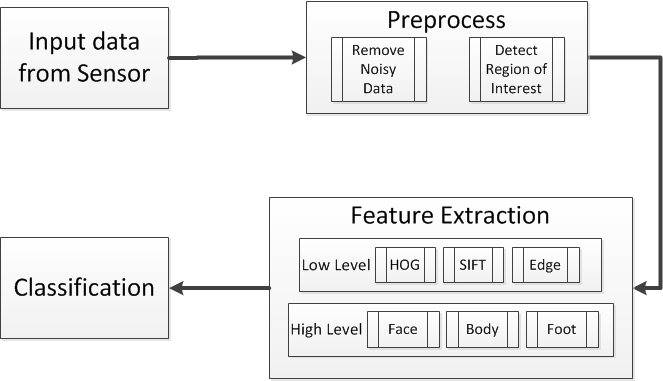
\includegraphics[scale=.8]{introduction/fig/IRflow.png}
	\caption{Major procedure for image recognition.}\label{fig:intro:irflow}
\end{figure}
\subsection{Preprocess}
Firstly, the optical property of an object is captured through its optical sensor of a digital camera and then the digital camera generates raw digital data of the image.
After receiving the raw data of a image from the sensor, preprocess is to generate a new image from the source image. This new image is similar to the source image, but differs from it considering certain apsects, e.g. the new image has smoother edge, better contrast and less noise. 
Here, some \textit{pixel operations} and \textit{local operations} are used to improve the contrast and remove the noise.  

Another important operation of preprecess is segmentation according to the object, i.e. finding the region of interest. Images used for recognition should be aligned, making the target object appear in the central of the image and remove those irrelevant area.

The result of preprocess has great impact on the final result of the recognition. Clear and noise free images can make the feature extraction more effective and significantly improve the final classification accuracy.

\subsection{Feature Extraction}
Feature extraction is used to extract the optical properties of an image and represent interesting parts of an image from the raw image data as a compact feature vector. The feature vector is then used for either training the classifier or recognition. Therefore, feature extraction is the most important part for image recognition. The quality of the features extracted from a image have great impact on the recognition result. There are two major streams for feature extraction: the hand engineered method and representation learning method.
\subsubsection{Hand Engineered Feature}
Hand engineered features are typically low level and local features.
Low level features are extracted according to some optical properties of an image. These features are low level / local features. There is a widely agreement that local features are an efficient tool for object representation due to their robustness with respect to occlusion and geometrical transformations \cite{van2006coloring}. Common low level hand engineered features include Histogram of Oriented Gradients (HOG) \cite{dalal2005histograms}, Scale Invariant Feature Transform (SIFT) \cite{lowe1999object}, Speeded Up Robust Features (SURF) \cite{bay2006surf}, Local Binary Patterns (LBP) \cite{ojala2002multiresolution}, and color histograms \cite{birchfield1998elliptical}. Feature descriptors obtain from these low level features refer to a pattern or distinct structure found in an image, such as a point, the edges, or some small image patches. They are usually associated with an image patch that differs from its immediate surroundings by texture, color, or intensity. What the feature actually represents does not matter. We know that it is distinct from its surroundings.
\begin{figure}[h]
	\centering
	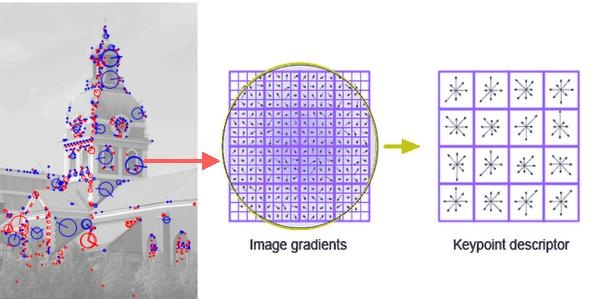
\includegraphics[scale=.6]{introduction/fig/sift.jpg}
	\caption{Feature extraction using SIFT.}\label{fig:intro:sift}
\end{figure}
These low level features can be used directly for recognition. However, since they just represent certain local properties of an image and are not discriminative enough for recognition, discriminative high level features can be further learned by combining the low level features using some algorithms such as bag-of-visual words\cite{lazebnik2006beyond}. 

\subsubsection{Representation Learning}
Representation learning is mainly described by Deep Learning 
algorithms\cite{krizhevsky2012imagenet} or Auto Encoders \cite{bengio2007scaling}. The ideas is to learn a group of filters that are able to capture various kinds of features to discern one category of images from the another category with some supervised or unsupervised algorithm. Typically in representation learning, features are learned hierarchically from low-level features to high level ones automatically. 
Learning representation from an image can start from either low level hand-crafted features (for Auto Encoders) or raw pixels of an image (for Deep Learning). 
\begin{figure}
	\centering
	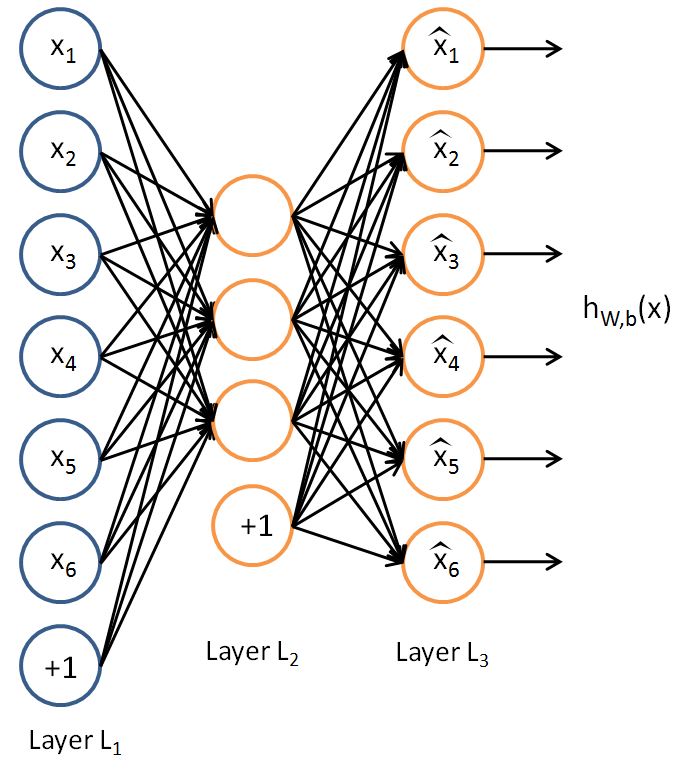
\includegraphics[scale=.3]{introduction/fig/sparsecoding.png}
	\caption{General Scheme of Auto Encoders. L1 is the input layer, possibly raw-pixel intensities. L2 is the compressed learned latent representation and L3 is the reconstruction of the given L1 layer from L2 layer. AutoEncoders tries to minimize the difference between L1 and L3 layers with some sparsity constraint.}\label{fig:intro:sparse}
\end{figure}

\textbf{Auto Encoders} are widely used to combine different types of low level feature. The outputs of the Auto Encoders are some latent representations. These latent representations are learned from the given images that have lowest possible reconstruction error. Even though the high level representations from Auto Encoders are learned by minimizing the reconstruction errors, they are still not robust enough to handle all kinds of variance of the objects in some tasks.

\textbf{Deep Learning} is the most popular approach for learning representations. It has been widely used for all kinds of image recognition tasks and achieved the state-of-the-art performance on some large scale image recognition tasks, such as ILSVRC and The PASCAL Visual Object Classes Challenge (PASCAL VOC). 
Convolutional Neural Networks (CNN) is the most popular deep learning model for the image recognition tasks\footnote{Deep CNNs are sometimes considered as the end-to-end classifier while learning the feature representation and discriminative classifier simultaneously. However, the feature representation learned from deep CNNs can still achieve good results with other classifiers and here we consider it as a feature extractor rather than a classifier.}. The first deep CNN that had great success on image recognition is the LeNet proposed by Y.LeCun in 1989 \cite{lecun1989backpropagation}. Backpropagation was applied to Convolutional Neural networks with adaptive connections. This combination, incorporating with Max-Pooling and speeding up on graphics cards has become an important part for  many modern, competition-winning, feedforward, visual Deep Learners. Deep CNNs have been widely used as the feature extractor for all kinds of images recognition tasks and proven to be the most powerful method of feature extraction.
\begin{figure}
	\centering
	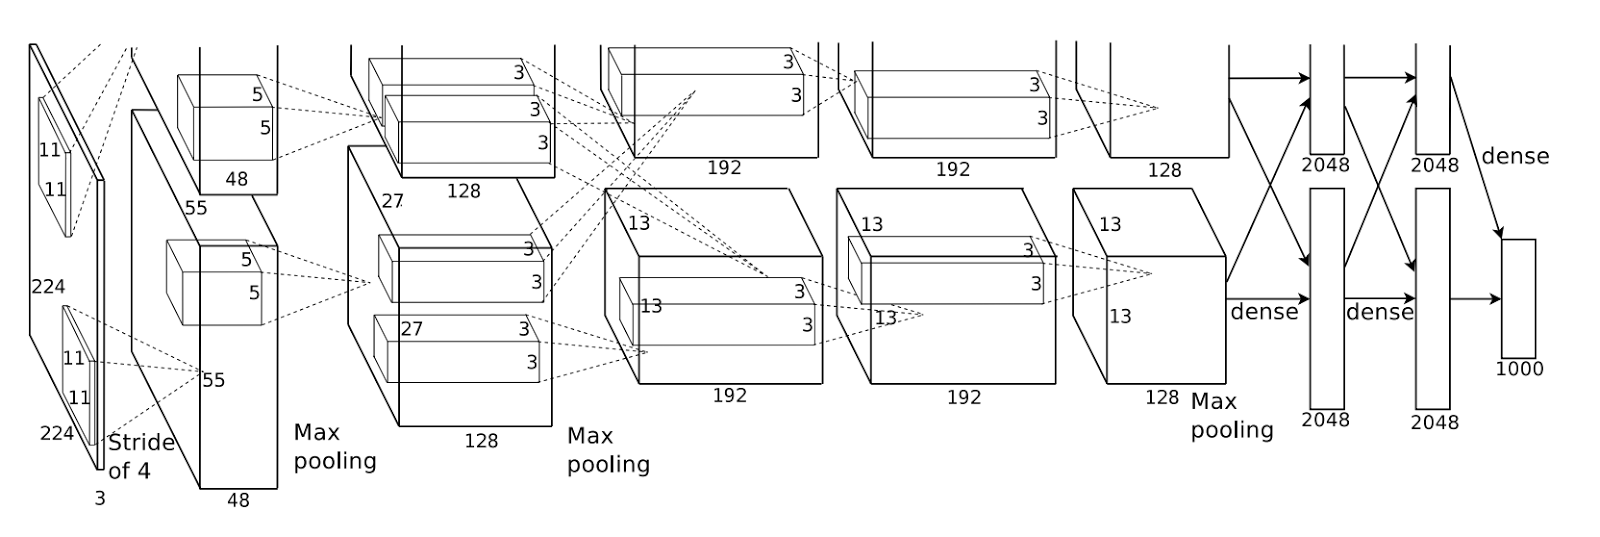
\includegraphics[scale=.3]{introduction/fig/alexnet.png}
	\caption{The architecture of ALEXNET (adopted from \cite{krizhevsky2012imagenet}).}\label{fig:intro:alex}
\end{figure}

\subsection{Classification}
After extracting feature representation from the images, a classifier is used to train a recognition model as well as for predicting the new coming images. A supervised model is always used for training the recognition model. Discriminative Classifier such as Support Vector Machine (SVM) is widely used as the classifier for recognition \cite{cristianini2000introduction}. As we mentioned before, in order to capture different variances of the images for one category, the size of the feature representation for an image is usually very large. In order to avoid overfitting, the size of the training set should be at least the same size of the feature representation as well. Some classifiers such as Bayesian method or decision tree require to consider the correlations between each feature and the class labels and suffer from the large feature dimension. However, Discriminative Models\cite{bottou2010large} are more convenient for training. Discriminative Models can be effectively optimized with stochastic gradient descent and are suitable for the large training set. 

However, to capture all variance of an object, training a good recognition model requires abundant data when we learn a model from scratch. With the limited training data, it is difficult to achieve a good classification performance. Transfer learning is an effective way to solve this problem by utilizing the knowledge from previous tasks. In this thesis, we focus on how to transfer the knowledge from the source domain for recognition tasks. The methods proposed in chapter \ref{sec:pakdd} and chapter \ref{sec:aaai} mainly focus on the stage of classification while the method in chapter \ref{sec:cnn} focuses on both feature representation learning and classification.




\section{Approaches in Visual Transfer Learning and the Limitations}
As we mentioned before, research of visual transfer learning focuses on designing classifiers that can leverage the source knowledge effectively. In this section, we briefly review methods for the visual transfer learning and show the limitation of previous work. 
\subsection{Intuition for Visual Transfer Learning}
The intuition of visual transfer learning comes from our human recognition mechanism. For our human, all the information acquired is stored in our memory. These information are organized according to the properties. When we see a new concept, we don't treat it isolated, but connect it to certain previous knowledge we stored in our memory. By comparing a new concept with the organized information in our memory, we can capture the property of a new concept effectively. When referring to visual tasks, several examples can be given to show this cognitive ability. For instance, when we describe the animal "okapi" (see Figure \ref{fig:intro:multi}), we would probably say that: okapi has a body of a horse, legs of the zebra and a head of giraffe. People who never see a zebra could instantly have a rough idea of a zebra. 

\begin{figure}
	\centering
	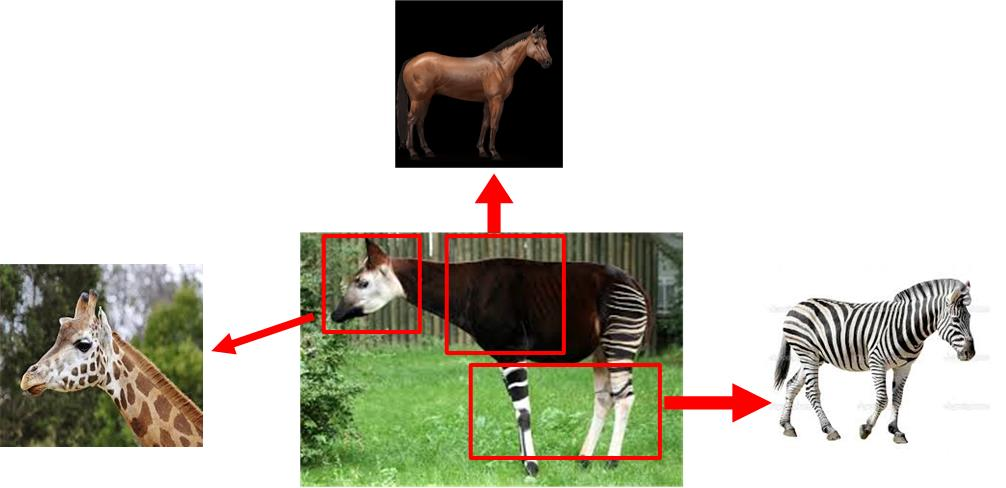
\includegraphics[scale=.6]{introduction/fig/multiple.jpg}
	\caption{An intuitive description for human to learn new concept: an okapi can be roughly described as the combination of a body of a horse, legs of the zebra and a head of giraffe.}\label{fig:intro:multi}
\end{figure}

This indicates that to learn a concept effectively, we should be able to make use of the gained knowledge instead of learn it from scratch. This process is commonly referred to as transfer learning\cite{pan2010survey}. Traditional machine learning methods work under the common assumption: training data and testing data are drawn from the same feature space and same distribution. 
In transfer learning, the test data can come from a different distribution. The data from the original distribution is called source data, and data from the new distribution is called target data. Transfer learning is used to utilize the source knowledge from the source data to help building the new model to classify the target data. 

\subsection{Approaches for Visual Transfer Learning}
Successfully leveraging the source knowledge can greatly improve the performance of the target model. In general, the more related the source and target domain are, the more useful the source knowledge is and the more benefit the target model can get. Leveraging unrelated knowledge cannot help to improve the performance of the target model or even hurt the it. Therefore, the key issue for visual transfer learning is to identify the relatedness of the source and target domain. The major approaches for Visual Transfer Learning consists of two main direction: Distribution Similarity Measurement and Instance Reuse.

\begin{itemize}
	\item \textbf{Distribution Similarity Measurement}. The core idea of transfer learning is to leverage the related source knowledge. The more related the source is, the better transfer performance we can achieve. Thus, measuring the the relatedness of the source knowledge is an important part in transfer learning especially where there are multiple sources. A straight-forward approach to identify the relatedness of the source and target domain is to measure their similarity directly. Measuring the data discrepancy through some statistical measurements such as \textbf{Maximum Mean Discrepancy} (MMD) \cite{duan2009domain}, has been a popular way to identify the source and target domain. MMD reflects the distance of two data distributions in the Reproducing Kernel Hilbert Space (RKHS) \cite{aronszajn1950theory}.
	\item \textbf{Instance Reuse}\cite{lim2012transfer}. Generally, we apply transfer learning under the scenario where the target data is scarce and we are not able to build the target model alone with the target data. A simple solution is to ``borrow" some of the data from the source domain and use it to build the target model together with the target data. This approach can directly increase the size of the data in the target domain and effectively improve the performance of the target model. For example, \textbf{Feature Transformation} \cite{duan2012learning} can overcome the data distribution mismatch in different domains and project the data into the same augmented space and thus can increase the training data for the target task as well (see Figure \ref{fig:intro:trans}).
\end{itemize}

\begin{figure}
	\centering
	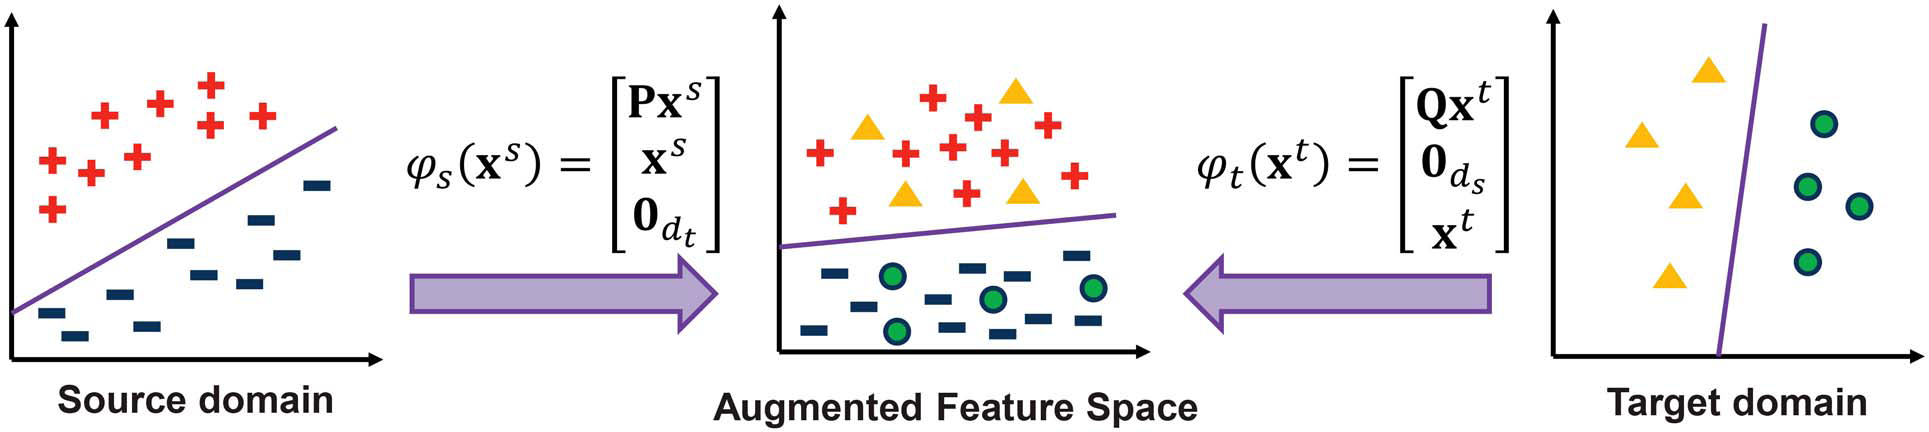
\includegraphics[scale=.3]{introduction/fig/transformation.png}
	\caption{Feature transformation. Transform the data in different domains into a augmented feature space.}\label{fig:intro:trans}
\end{figure}

\subsection{Limitation of Previous Methods}
From the review of the approaches for Visual Transfer Learning we can see that
most previous methods require access to the source data to obtain the source knowledge. However, in many practical problems, these previous approaches may not be as convenient as we thought due to the following reasons:

\begin{itemize}
	\item \textbf{Data accessibility}. The source data may not be able to access for some tasks. For example, clinical database is not allowed to access for general publics due to the privacy. Disclosure obligations and will to share the databases are also two important reasons that make the source data inaccessible.
	\item \textbf{Size of the source data}. Besides data accessibility, many previous methods \cite{daume2009frustratingly}\cite{duan2012learning} require to access to each of the individual source instance to obtain the source knowledge which is ineffective for many large source domain. For example, it is almost impossible to measure the MMD for some large source domain which contains hundreds of thousands instances.
\end{itemize}

From above we can see that these previous methods can successfully leverage the source knowledge under the assumption that the source data are freely accessible and relatively small. However, this assumption could fail in real applications. In some cases, the source data could be private (such as the clinic data from patients) and therefore, could not be shared with public. Moreover, those large source dataset generally contains more knowledge and information compared to the small ones and thus can better improve the transfer performance of the target task. However, obtaining the similarity measurement of these large dataset with those previous methods can be tedious and inefficient. It is important to find a way to leverage the source knowledge without accessing to the source data.

In this thesis, we assume that we can freely access to the source model trained from the source data and thus leverage the knowledge from the model instead. Using the source model for transfer learning can successfully avoid the two issues discussed above. Source model can contain as much knowledge as the source data while without containing any information regarding to the individual instance. Therefore, the owner of the source data does not have to worry about the leak of the privacy. For those large source dataset such as ILSVRC containing millions of images, a trained source model is normally a few megabytes and public available. Therefore, leveraging the source knowledge from source model instead of the source data itself is more practical for real visual transfer learning applications.
%%%%%%%%%%%%%%%%%%%%%%%%%%%%%%%%%%%%%%%%%%%%%%%%%%%%%%%%%%%%%%%%%%%%%%%%%%%%%%%%%

\section{Main Contribution}
In this section, we discuss the challenges that we may encounter when we can only access the source model. Then we demonstrate the learning scenarios and proposed solutions in this thesis.

\subsection{Challenges}
Despite for the general challenges in transfer learning, in our HTL settings, there are some new challenges in this thesis.

The first challenge is \textbf{knowledge representation}, i.e. how to obtain the source knowledge when we are not able to access to the source data. When source data is accessible, the source knowledge is relatively explicit and we can easily obtain the source knowledge by either analyzing the source data distribution or make use of the source data to help training the target mode. The knowledge of the source domain is implicit and encoded in the source model using certain learning algorithms. How to effectively extract the source knowledge from the models is challenging.

The second challenge is \textbf{knowledge expressiveness}, i.e. how to leverage the source knowledge to help training the target model. As the source knowledge is implicit, how to effectively leverage the source knowledge and improve the transfer performance is also important. We also expect that the source knowledge extracted from the source model should be as general as possible so that the source knowledge can be extracted from different types of source model. Therefore, our transfer learning algorithm can work in many situations. 

The last challenge is \textbf{knowledge regularization} i.e. how to guarantee the performance of our transfer method. 
Humans appear to have mechanisms for deciding when to transfer information, selecting appropriate sources of knowledge, and determining the appropriate level of abstraction \cite{torrey2009transfer}. 
A basic criterion for the knowledge transfer process is that leveraging the knowledge from the source model should not hurt the performance of the target model. Negative transfer \cite{pan2010survey} happens when the performance of target model degrades after receiving the knowledge from the source domain and how to avoid negative transfer is still an open question to all transfer learning researchers. The absence of the source data makes the situation more complicated.

\subsection{Two Transfer Learning Scenarios}
In this thesis, we mainly focus on two transfer learning scenarios: inductive transfer learning for new classes and domain adaptation. The definition of the two scenarios is as follows:
\begin{definition}{\textbf{Domain Adaptation}}
	Let $X$ be the input space and $Y$ be output space. Given the source domain $D_s$ and the target learning task $D_t$ with marginal distribution $P(X_s)$ and $P(X_t)$, we assume that $D_s$ and $D_t$ share the same conditional distribution $P(Y|X)$. The goal of Domain Adaptation is to learn the $P(X_t|Y_t)$ for the target task with the help of $D_s$.
\end{definition}

\begin{definition}{\textbf{Inductive Transfer Learning}}\cite{pan2010survey}
	Given a source domain $D_s$ and the source learning task $T_s$, a target domian $D_s$ and the target learning task $D_t$, inductive transfer learning aims to help improve the learning of the target task function $f_t(\cdot)$ in $D_t$ using the knowledge from $D_s$ and $D_s$ where $D_s \neq D_t$.
\end{definition}

The major difference between the two transfer learning scenarios is that in inductive transfer learning, the source and target tasks are two different but related tasks (e.g. from sport car to heavy truck) while in domain adaptation, the source and target tasks are the same task but with different marginal distributions (e.g. from the animation dog to the real dog). 

\begin{figure}[h]
	\centering
	\subfloat[Domain Adaptation]{\includegraphics[scale=.4]{introduction/fig/da.png}}
	\qquad
	\subfloat[Inductive transfer learning the new class]{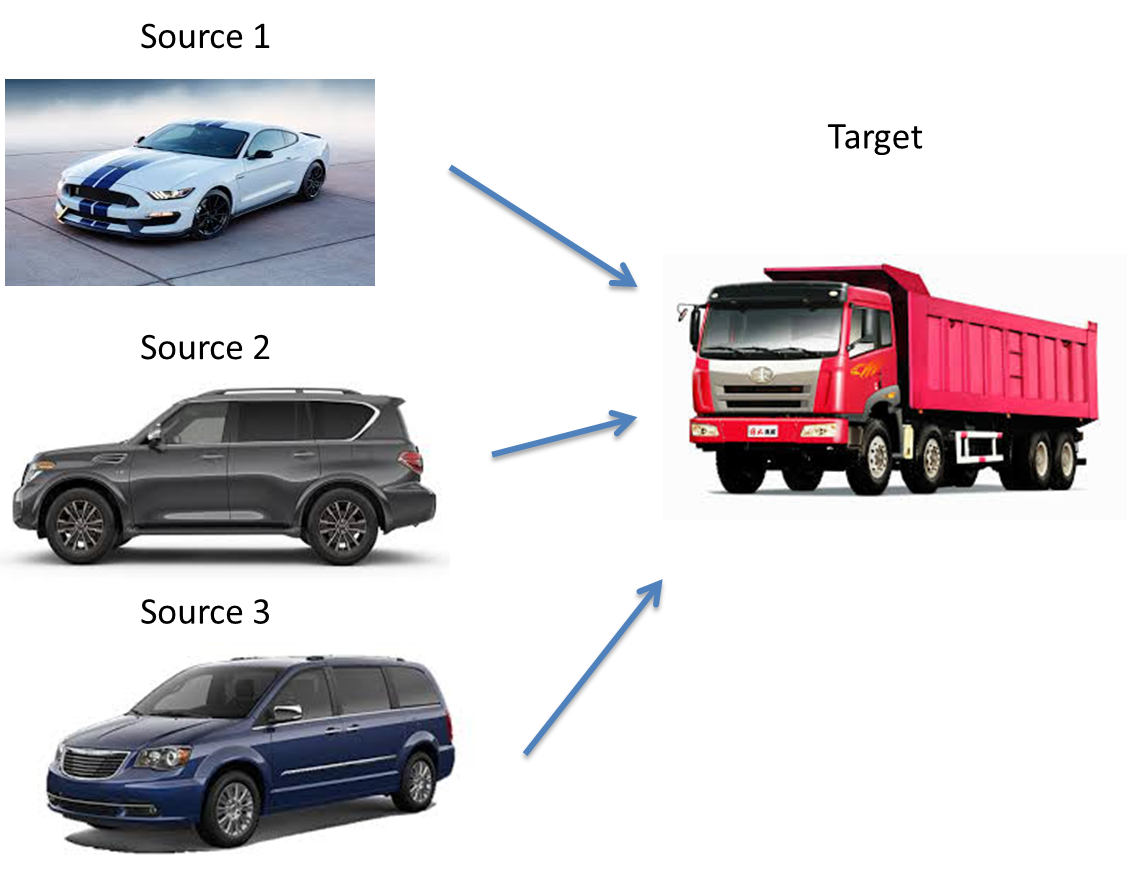
\includegraphics[scale=.33]{introduction/fig/ind.png}}
	\caption{Difference between two transfer learning scenarios}\label{fig:intro:cmp}
\end{figure}


\subsection{Proposed Methods}
There are three methods proposed in this thesis, one in inductive transfer learning for new classes and two methods in domain adaptation.


In chapter \ref{sec:pakdd}, we extend the previous methods in HTL which are limited to using SVMs as the source model and propose a novel method \textbf{Effective Multi-class Transfer Learning} (EMTLe) for supervised domain adaptation. We use the output of the source model as the auxiliary bias to adjust the target model. Here, the output of the source model is used as the prior to adjust the decision for the target model. As long as we can set a proper weight to the prior knowledge, the source model can serve well for the target task. Because we only require the source model to provide its decision, we can treat it as a black-box model and EMTLe can leverage the source model from any source classifier that can generate the class probability of an example.

In chapter \ref{sec:aaai}, we investigate the problem of semi-supervised domain adaptation where most of the data in the target task are unlabeled and propose a novel framework \textbf{Generalized Distillation Semi-supervised Domain Adaptation} (GDSDA). In GDSDA, the source model generates ``soft labels" for the target data and can improve the performance together with the true labels from target task. Arguably, we use the imitation parameter to determine the relative importance of the soft label and true label. Then we propose GDSDA-SVM that can determine the imitation parameter autonomously through cross-validation.

In chapter \ref{sec:cnn}, we use the deep neural network to solve the transfer learning problem for food recognition. We use GoogLeNet trained from ImageNet of 1000 classes as our source model and two food databases as our target task, containing 101 classes and 265 classes respectively. In this chapter, we don't treat the source model as a black-box. Instead, we can obtain the parameters of the original GoogLeNet. We re-use the parameters in the original GoogLeNet as the prior and fine-tune it on our target task to achieve the improved performance. By re-using and fine-tuning the parameter, i.e. features from source tasks, we can effectively learn new categories of the target task. We show that without accessing the source data, we can still achieve better performance compared to previous methods.
\section{Summary}
In this chapter, we briefly introduced the problems that are solved in this thesis. We first demonstrate the procedure for image recognition and introduce some previous work for visual transfer learning. Then we pointed out the limitations of the previous work and proposed our methods under two transfer scenarios.\label{sec:intro}
\chapter{Related Work}\label{sec:works}
In this chapter, we review some previous work related to ours. In Section \hl{we review......}
\section{Classifiers for Image Recognition}\label{sec:relat:linear}

In our scenario, we have to face the problem of image recognition. Due to the large dimension of the feature representation for each image as well as the size of training image, manual classification is hopeless. As we mentioned in Section \ref{sec:intro:over}, a recognition model is used to distinguish the objects from different categories automatically trained by supervised learning. In this section, we introduce the classifiers we used in this thesis.

\subsection{Binary Classification and Multi-class Classification}

In image recognition, we train a recognition model from a set of training images along with their labels provided. The labels are predefined in a category space. Thus, the task of image recognition is to classify each image as one predefined category. If there are only two categories, this recognition task is called binary classification. For the task recognizing the objects from more than two categories, the recognition task is called multi-class classification \cite{aytar2011tabula} \cite{krizhevsky2012imagenet}.  

Here, we give a formal definition of the scenario for binary and multi-class classification. Generally, we can decompose the multi-class learning task into a set of binary scenarios by training a binary classifier for each class, e.g. One-VS-Rest strategy (see figure \ref{fig:related:ovsa})\cite{rifkin2004defense} \cite{tsoumakas2006multi}.

The binary scenario for classification can be defined as follow: given a dataset from domain $\mathcal{X} \times \mathcal{Y}$ where $\mathcal{X}$ is the input feature representation and $\mathcal{Y}$ is the binary label set $\{1,-1\}$ (for some classifier, $\{1,0\}$ is also used). We usually use the label $1$ to denote the examples belong to one certain category and -1 to denote examples not belong to that category. 
We assume that the training image set $D_{train}=\{(x_i,y_i)\} \subset \mathcal{X} \times \mathcal{Y}$ and the test image set $D_{test}=\{(x^t_i,y^t_i)\}\subset \mathcal{X} \times \mathcal{Y}$ are given and separated from each other. Each pair $(x_i,y_i)$ denotes the input feature representation $x_i$ and its corresponding label $y_i$ for the $i$\textit{th} image in the both set. Our goal of the classification problem is to learn a decision function $f:\mathcal{X} \rightarrow \mathcal{Y}$ from the training set $D_{train}$ such that $f$ can achieve good performance on both $D_{train}$ and $D_{test}$. 

\begin{figure}
	\centering
	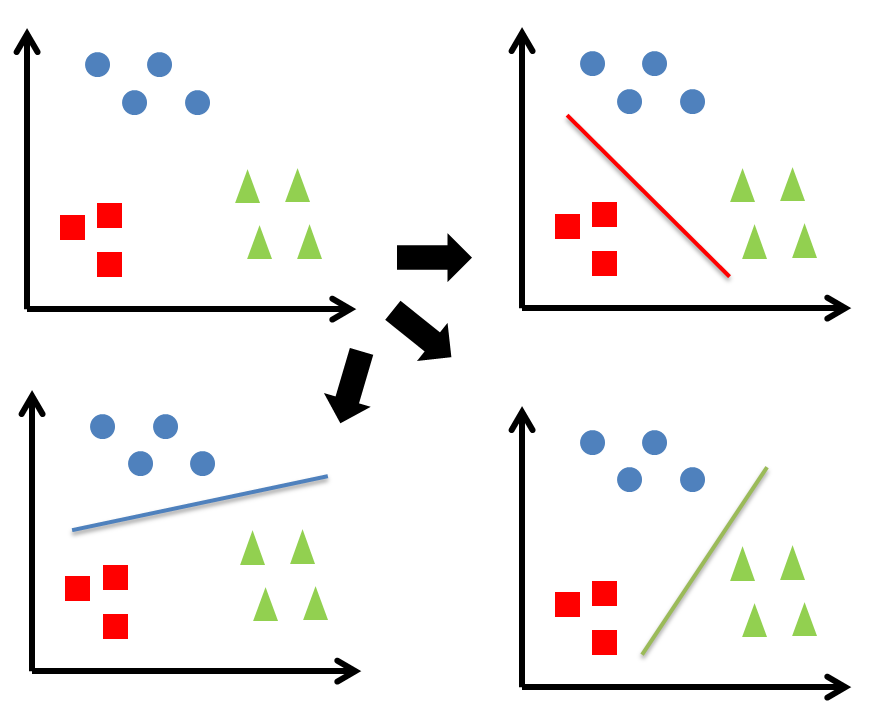
\includegraphics[scale=.8]{relatedwork/fig/ovsa.png}
	\caption{One-vs-Rest strategy for multi-class scenario. A three classes problem can be decomposed into 3 binary classification sub-problems.}\label{fig:related:ovsa}
\end{figure}
\subsection{Softmax Classifier}
In this subsection, we will introduce a widely used linear classifier \textbf{Softmax classifier} in image recognition. Linear classifier is commonly used as the classification model for image recognition. Linear classifier achieves this by making a classification decision based on the value of a linear combination of the input feature representations of a image. A linear classifier consists of two parts: a score function and a loss function. The score function maps the input data into the class scores and the loss function that quantifies the agreement between the predicted scores and the ground truth labels. Linear classifier often works very well when the number of dimensions of the input is large. Therefore, it is widely used as the classifier for image recognition, especially as the classifier for Convolutional Nueral Networks \cite{lecun1989backpropagation}. 

Typically, Softmax classifier is widely used for multi-class image classification.
Softmax classifier (also called multinomial logistic regression) is a generational form of logistic regression for the multi-class scenario. As logistic regression can only handle the binary classification scenario, Softmax classifier adapts the one-vs-rest strategy where several logistic regression models are trained for each class. 

Given a training set $\{(x_1,y_1),(x_2,y_2),...,(x_m,y_m)\}$, we assume the label $y_i \in \{1,0\}$ and the input feature $x_i \in \mathcal{R}^n$. For each binary logistic regression model, The score function takes the form:
\begin{equation}
{f_w}(x) = \frac{1}{{1 + \exp ( - {w^T}x)}}
\end{equation}
and the parameters $w$ are optimized to minimize the following loss function:
\begin{equation}
l(w) =  - [\sum\limits_{i = 1}^m {{y_i}\log {f_w}({x_i}) + (1 - {y_i})} \log (1 - {f_w}({x_i}))]\label{eq:logistic:loss}
\end{equation}

For Softmax classifier, it is used to handle the multi-class classification problem and suppose there are $N$ classes. Therefore, $y$ can take from $N$ different values $\{1,2,3,...,N\}$ instead of just two. For a given test example $x$, the score function estimate the probability $P(y=n|x)$ for each value of $n = 1,2,3,...,N$, i.e. estimate the probability that each score assigns the input $x$ to the $N$ classes associated to the $N$ different possible values. Thus, the score function will output a $N$-dimensional vector providing $N$ estimated probabilities whose sum of elements is 1. The $N$ dimensional output of the score function can be generated according to the following form:
\begin{equation}
{f_w}\left( x \right) = \left[ \begin{array}{l}
P\left( {y = 1|x;w} \right)\\
P\left( {y = 2|x;w} \right)\\
...\\
P\left( {y = n|x;w} \right)
\end{array} \right] = \frac{1}{{\sum\nolimits_{j = 1}^N {\exp \left( {{w^{(j)T}}x} \right)} }}\left[ \begin{array}{l}
\exp \left( {{w^{(1)T}}x} \right)\\
\exp \left( {{w^{(2)T}}x} \right)\\
...\\
\exp \left( {{w^{(N)T}}x} \right)
\end{array} \right]
\end{equation}
Here $w^{(1)T},w^{({2})T},...,w^{({N})T}$ are the parameters of the Softmax classifier model. The term $\frac{1}{{\sum\nolimits_{j = 1}^N {\exp \left( {{w^{(j)T}}x} \right)} }}$ is called the normalization term so that the $N$ distributions sum to 1.

To optimize the parameters $w^{(1)T},w^{({2})T},...,w^{({N})T}$, the cross-entropy loss used for the Softmax classifier is defined as:
\begin{equation}
J(w) =  - \left[ {\sum\limits_{i = 1}^l {\sum\limits_{k = 1}^N {\ell\left\{ {{y_i} = k} \right\}\log \frac{{\exp \left( {{w^{(k)T}}x_i} \right)}}{{\sum\nolimits_{j = 1}^N {\exp \left( {{w^{(j)T}}x_i} \right)} }}} } } \right] \label{eq:softmax:loss}
\end{equation}
Here $\ell{x}$ is the 0-1 loss function:
\begin{equation}
\ell \{ x\}  = \left\{ {\begin{array}{*{20}{c}}
	1&\text{$x$ is true}\\
	0&\text{$x$ is false}
	\end{array}} \right. 
\end{equation}
It is noted that Eq \eqref{eq:softmax:loss} is a generalized form of Eq \eqref{eq:logistic:loss}. Minimizing Eq \eqref{eq:softmax:loss} can be interpreted as minimizing the negative log likelihood of the correct class, which is equivalent to performing Maximum Likelihood Estimation (MLE) \cite{johansen1990maximum}.

The minimum of $J(w)$ can be obtained by gradient descent method while taking the gradient:
\begin{equation}
\nabla J({w^{(n)}}) =  - \sum\limits_{i = 1}^l {\left[ {{x_i}\left( {\ell \left\{ {{y_i} = n} \right\} - \frac{{\exp \left( {{w^{(k)T}}x_i} \right)}}{{\sum\nolimits_{j = 1}^N {\exp \left( {{w^{(j)T}}x_i} \right)} }}} \right)} \right]} 
\end{equation}

\subsection{Support Vector Machines}
In this subsection, we will review another widely used discriminant classifier, \textbf{Support Vector Machine} (SVM) \cite{cristianini2000introduction}. SVM is another classifier that has been adoptive in many image recognition tasks \cite{coates2011analysis} \cite{schuldt2004recognizing} \cite{yang2009linear}. In this thesis, we also use a classifier based on SVM. We will give a detailed description of SVM. 

As we mentioned before, the linear classifier consists of two parts: the score function and loss function. SVM classifier can be divided into two categories based on their score function: linear SVM that uses a linear discriminant function and kernel SVM that uses kernel function. Kernel SVM can be considered as a extension version of linear SVM where kernels are used for calculate the scores of the inputs. Another difference for between linear and kernel SVM is linear SVM can be solved on the primal problem while kernel SVM is mostly optimized on its dual \cite{cristianini2000introduction} \cite{shalev2011pegasos}.

First, we will introduce the linear SVM. Linear SVM uses the simplest representation of a score function by taking the linear combination of the input vector:
\begin{equation}\label{eq:relation:score}
f(x) = w^Tx+b
\end{equation}
where $w$ is called the weight vector and $b$ is called the bias. In a binary scenario, for the input example $x$ and the class labels $y \in \{c1,c2\}$, $x$ is assigned to class $c1$ if $f(x) \geq 0$ and $c2$  otherwise. Therefore, the corresponding decision surface is defined by $f(x)=0$. For two points $x_1$ and $x_2$ lie on the decision surface, we have $f(x_1)=f(x_2)=0$. Then we can have $w^T(x_1-x_2)=0$ and hence the weight vector $w$ is orthogonal to every point lying within the decision surface, i.e $w$ determines the orientation of the decision surface. Similarly, if $x$ lies on the decision surface, the normal distance from the origin to the decision surface is given by:
\begin{equation}
\frac{w^Tx}{||w||}=-\frac{b}{||w||}
\end{equation}
Therefore, we can see that, the location of the decision surface is determined by the bias $b$.
\subsubsection{Hard Margin SVM}
Hard margin SVM is used to find the optimal solution for the data sets that are linear separable. 
Given a set of n training points $(x_1,y_1),(x_2,y_2),...,(x_n,y_n)$ where $y_i \in \{1,-1\}$, we expect to find a decision surface that can separate the data from two classes. However, when the data from these two classes can be linearly separated, there could be several decision surfaces that can separate the data. The idea of SVM is to choose the maximal margin decision surface so that the distance between these two classes is as large as possible (called maximal margin hyperplane). For example, in figure \ref{fig:relate:svm}\subref{fig:relate:svma}, $H2$ and $H3$ are two candidate decision surface that can separate the data. However, $H3$ is has the largest distance to all the data from two classes and SVM will choose $H3$ as the optimal hyperplane. 

\begin{figure}
	\centering
	\subfloat[Different sparating hyperplanes]{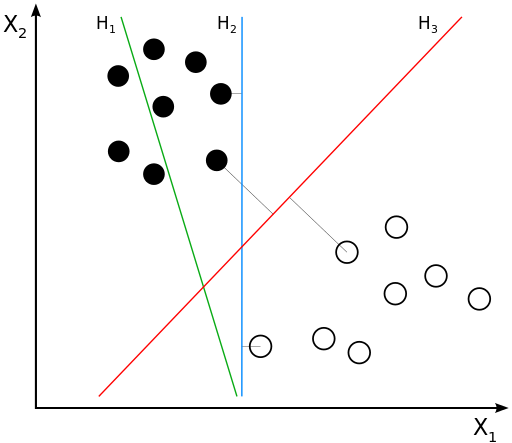
\includegraphics[width = 0.45\textwidth]{relatedwork/fig/svm2.png}\label{fig:relate:svma}}
	\subfloat[Max-Margin hyperplanes]{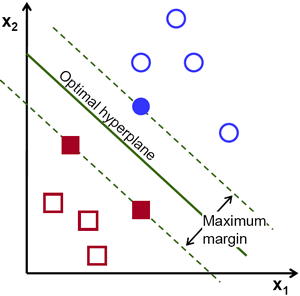
\includegraphics[width = 0.4\textwidth]{relatedwork/fig/svm1.png}}
	\caption{Support Vector Machine}\label{fig:relate:svm}
\end{figure}
The optimal hyperplane can be found by minimizing the following objective function:
\begin{equation}
\begin{aligned}
\min \qquad & ||w||^2\\
\text{s.t.}\qquad & y_i(w^Tx_i+b) \geq 1 \quad \text{for all } 1\leq i \leq n
\end{aligned}
\end{equation}
\subsubsection{Soft Margin SVM}
In real world application, most data are not linear separable. Therefore, SVM introduce the concept of slack variable to handle this situation. Slack variable is defined as:
\begin{equation}
\xi_i  = hinge(x_i) = \max (0,1-y_i(w^Tx_i+b))
\end{equation}
The value of slack variable is 0 if the example $x_i$ lies on the correct side of the margin. For those data on the wrong side, its value is proportional to the distance from the correct margin.
\begin{figure}
	\centering
	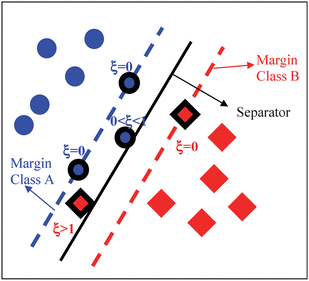
\includegraphics[scale =1.2]{relatedwork/fig/slack.png}
	\caption{Slack variables for soft-margin SVM}
\end{figure}

Therefore, to find the parameters of hyperplane, i.e. weight vector $w$ and bias $b$, soft-margin SVM minimize the following loss function:
\begin{equation}\label{eq:related:softsvm}
\begin{aligned}
\min \qquad &  \frac{\lambda}{2}||w||^2+\frac{1}{n}\sum_{i}^{n}\xi_i\\
\text{s.t.}\qquad & y_i(w^Tx_i+b) \geq 1-\xi_i \\
& \xi_i \geq 0     \quad \text{for all } 1\leq i \leq n
\end{aligned}
\end{equation}
The objective function is called primal of SVM. A stochastic sub-gradient descent can be used to find the optimal solution for eq. \eqref{eq:related:softsvm} effectively \cite{shalev2011pegasos}. 
\subsubsection{Kernel SVM}
Linear soft-margin SVM works well when number of features is larger than number of training examples. However, when the size of the training example is larger than the features, kernel SVM (such as Gaussian Kernel) with proper parameters outperforms linear SVM \cite{keerthi2003asymptotic}.
\begin{figure}
	\centering
	{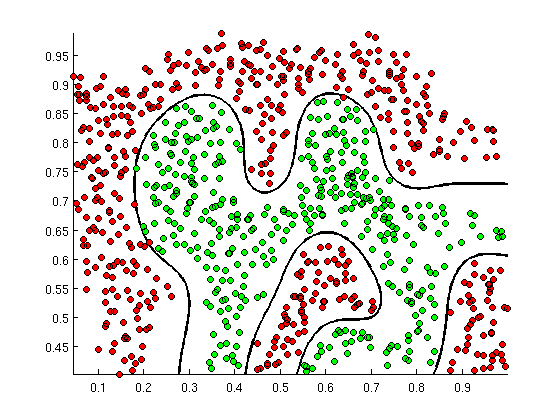
\includegraphics[width = 0.8\textwidth]{relatedwork/fig/non-linear2.png}}
	\caption{The hyperplane of SVM with RBF kernel for non-linear separable data.}\label{fig:relate:nonlinear}
\end{figure}

The idea of kernel was first introduced into pattern recognition by Aizerman \textit{et. al.} \cite{aizerman1964probability}. When the size of the training examples are significantly larger than the dimension of the input features and the distribution become more complex, these data can not be easily separated by a straight line in the feature space.
Instead of obtaining the optimal hyperspace in the input feature space, kernel SVM tries to map the inputs into a high-dimensional feature spaces and find the optimal hyperplane in the high-dimensional feature spaces. Given a feature space mapping $\phi(x)$, the score function for kernel SVM can be re-written as:
\begin{equation}\label{eq:relation:kernel}
f(x) = w^T\phi(x)+b
\end{equation}
From eq \eqref{eq:relation:kernel} we can see that, when we take the identity mapping $\phi(x) = x$, the kernel SVM becomes a linear SVM. Therefore, the linear SVM can be considered as a special case of kernel SVM where identity mapping is used as the kernel. The loss function of kernel SVM is almost identical to eq. \eqref{eq:related:softsvm} except for replacing the term $x$ with $\phi(x)$: 
\begin{equation}\label{eq:related:primal}
\begin{aligned}
\min \qquad &  \frac{\lambda}{2}||w||^2+\frac{1}{n}\sum_{i}^{n}\xi_i\\
\text{s.t.}\qquad & y_i(w^T\phi(x)_i+b) \geq 1-\xi_i \quad \\
& \xi_i \geq 0     \quad \text{for all } 1\leq i \leq n
\end{aligned}
\end{equation}
By introducing the Lagrangian term to the primal \eqref{eq:related:primal} and some transformation, we obtain the dual of kernel SVM function:
\begin{equation} \label{eq:related:dual}
\begin{aligned}
\max \qquad& \sum_{i}^{n}\alpha_i-\sum\limits_i^n {\sum\limits_j^n {{y_i}{y_j}{\alpha _i}} } {\alpha _j}\phi ({x_i})\phi ({x_j})\\
\text{s.t.} \qquad & 0 \leq \alpha_i \leq \frac{1}{\lambda}\\
& \sum_{i}^{n}y_i\alpha_i=0 \quad \text{for all } 1\leq i \leq n
\end{aligned}
\end{equation}
We can obtain the solution of \eqref{eq:related:dual} by Sequential Minimal Optimization (SMO) \cite{platt1998sequential} or Dual Coordinate Descent \cite{hsieh2008dual}.

There are several advantages of using SVM as the classifier: 
\begin{itemize}
	\item \textbf{Generalization ability.} SVM provides good generalization ability by maximizing the margin between the examples of the two classes. By setting the proper parameters and generalization grade, SVM can overcome some bias from the training set. Therefore, SVM is able to make correct prediction for unseen data. This ability can be very useful for image recognition as there is no image dataset that can cover all the transformation of the objects. Moreover,the idea of soft-margin makes it robust against noisy data.
	\item \textbf{Kernel transformation.} By introducing the non-linear transformation of the input, SVM can model complex non-linear distributed data. The kernel trick can greatly improve the computational efficiency.   
	\item \textbf{Unique solution.} The objective function of SVM is  convex. Compared to other methods, such as Neural Networks, which are non-convex and have many local minima, SVM can deliver a unique solution for any given training set and can be solved with efficient methods, like sub-SGD \cite{shalev2011pegasos} or SMO \cite{platt1998sequential}. 
\end{itemize}


\subsection{Convolutional Neural Networks}
Convolutional Neural Networks \cite{lecun1998gradient} is the most popular and powerful method for image recognition task. In this part, we introduce the history of Convolutional Neural Networks. The detail description of the Convolutional Neural Networks layers will be included in chapter \ref{sec:cnn}.

\subsubsection{Early Work with Convolutional Neural Networks}
The first simple version of Neural Networks (NNs) trained with supervised learning was proposed in 1960s  \cite{rosenblatt1958perceptron}\cite{rosenblatt1962principles}. Networks trained by the Group Method of Data Handling (GMDH) could be the first DL systems of the Feedforward Multilayer Perceptron type \cite{ivakhnenko1965cybernetic}\cite{Schmidhuber14}. Later, there have been many applications of GMDH-style
nets \cite{farlow1984self} \cite{ikeda1976sequential} \cite{kondo2008multi} \cite{witczak2006gmdh}.

Apart from deep GMDH networks, the Neocognitron, a hierarchical, multilayered artificial neural network, was perhaps the first artificial NN to incorporate the
neurophysiological insights \cite{fukushima1980neocognitron}. Inspired by Neocognitron, Convolutional NNs (CNNs) was proposed where the rectangular receptive field of a convolutional unit with given weight vector is shifted step by step across a 2-dimensional array of input values, such as the pixels of an image (usually there are several such filters). The results of the previous unit can provide inputs to higher-level units, and so on. Because of its massive weight replication,  relatively few parameters may be necessary to describe its behavior.

In 1989, backpropagation \cite{lecun1989backpropagation}\cite{lecun1998gradient} was applied to Convolutional Neural networks with adaptive connections \cite{lecun1989backpropagation}. This combination, incorporating with Max-Pooling and speeding up on graphics cards has become an important part for many modern, competition-winning, feedforward, visual Deep Learners. Later, CNNs achieved good performance on many practical tasks such as MNIST and fingerprint recognition and was commercially used in these fields in 1990s \cite{baldi1993neural} \cite{le1990handwritten}. 

In the early 2000s, even though GPU-MPCNNs wons several official contests, many practical and commercial pattern recognition applications were dominated by non-neural machine learning methods such as Support Vector Machines (SVMs).

\subsubsection{Recent Achievements with Convlutional Neural Networks}
In 2006, CNN trained with backpropagation set a new MNIST record of 0.39\% without using unsupervised pre-training \cite{marc2006efficient}. Also in 2006, an early GPU-based CNN implementation was introduced which was up to 4 times faster than CPU-CNNs \cite{chellapilla2006high}. Since then, GPUs or graphics cards have become more and more essential for CNNs in recent years. In 2012, a GPU implemented Max-Pooling CNNs (GPU-MPCNNs) was also the first method to achieve human-competitive performance (around 0.2\%) on MNIST \cite{ciresan2012multi}.

In 2012, an ensemble of GPU-MPCNNs (called AlexNet) achieved best results (top-5 accuracy at 83\%) on the ImageNet classification benchmark (ILSVRC2012), which contains 1000 classes and 1.2 million images \cite{krizhevsky2012imagenet}. After that, excellent results have been achieved by GPU-MPCNNs in image recognition and classification. Many attempts have been made to improve the architecture of AlexNet. With the help of high performance computing systems, such as GPUs and large scale distributed cluster, some improvements have been made by either making the network deeper or increasing the size of the training data  (with extra training example and data argumentation). By reducing the size of the receptive field and stride, Zeiler and Fergus improve AlexNet by 1.7\% on top 5 accuracy \cite{zeiler2014visualizing}. By both adding extra convolutional layers between two pooling layers and reducing the receptive field size, Simonyan and Zisserman built a 19 layer very deep CNN and achieved 92.5\% top-5 accuracy \cite{simonyan2014very}. After the AlexNet-like deep CNNs won ILSVRC2012 and ILSVRC2013, Szegedy et al. built a 22-layer deep network, called GoogLeNet and won the 1st prize on ILSVRC2014 for 93.33\% top-5 accuracy, almost as good as human annotation\cite{szegedy2014going}. Different from AlexNet-like architecture, GoogLeNet shows another trend of design, utilizing many $1\times 1$ receptive field. Recently, Wu et. al present an image recognition system by aggressive data augmentation on the training data, achieving a top-5 error rate of 5.33\% on ImageNet dataset\cite{wu2015deep}. Searchers from Google successfully trained an ingredient detector system based on GoogLeNet with 220 million images harvested from Google Images and Flickr \cite{malmaud2015s}.  

Besides its impressive performance on those huge datasets, MPCNNs shows some impressive results by fine-tuning the existing models on small datasets.Zeiler et al. applied their pre-trained model on Caltech-256 with just 15 instances per class and improved the previous state-of-the-art in which about 60 instances were used, by almost 10\% \cite{zeiler2014visualizing}. Chatfield et al. used their pre-trained model on VOC2007 dataset and outperformed the previous state-of-the-art by 0.9\% \cite{Chatfield14}. Zhou et al. trained AlexNet for Scene Recognition across two datasets with identical categories and provided the state-of-the-art performance using our deep features on all the current scene benchmarks \cite{NIPS2014_Zhou}. Hoffman et al. fine-tuned the MPCNNs trained from ImageNet with one example per class, showing that it is possible to use a hybrid approach where one uses different feature representations for the various domains
and produces a combined adapted model \cite{hoffman2013one}.

To summarize, in this section, we have briefly reviewed three types of classifier for image recognition, namely Softmax classifier, SVM and CNNs. Softmax classifier is typically used as the last layer of CNNs. SVM is a more general method for the classification task. Moreover, The generalization ability of SVM classifier can reduce the bias from the training data.

\section{An Overview of Visual Transfer Learning}
\hl{As we mentioned before, we use the transfer learning method to learn the self-defined categories. In this section, we review some problems transfer learning faces and the popular methods to learn new categories in transfer learning.} 
\begin{figure}
	\centering
	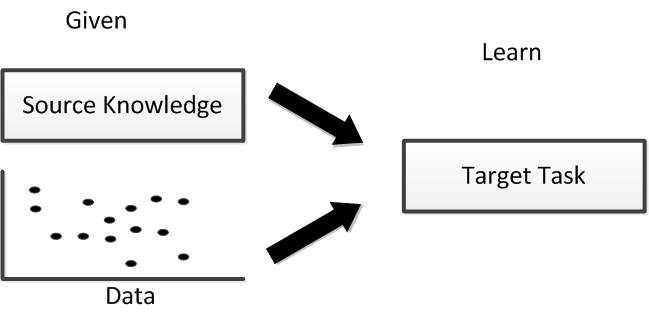
\includegraphics[scale =.7]{relatedwork/fig/transfer.png}
	\caption{Apart from the standard machine learning, transfer learning can leverage the information from an additional source: knoweldge from one or more related tasks.}
\end{figure}

Traditional machine learning algorithms try to build the classifiers from a set of training data and apply to the test data with the same distribution to the training data. In contrast, transfer learning attempts to change this by transfer the learned knowledge from one or several tasks (called source tasks) to improve a related new task (called target task).

Transfer learning can be categorized into 3 sub-settings: \textit{inductive transfer learning, transductive transfer leanring} and \textit{unsupervised transfer learning} based on the different situations of the source and target domains and tasks. \cite{pan2010survey}. We compared the differences of these three sub-categories and show them in Table \ref{tab:related:transfersetting}. \hl{Recalling our learning} self-defined category problem, we already obtained the source models from labelled source data and our goal is to utilize the knowledge from the source models and help us to train the models from a small set of labelled examples, i.e. examples from our self-defined categories. From Table \ref{tab:related:transfercmp} and \ref{tab:related:transfersetting} we can see that, our problem should be classified as inductive transfer learning. More specifically, it belongs to the multi-task transfer learning.

\begin{table}[htbp]
	\centering
	\caption{Relationship between traditional machine learning and different transfer learning settings}
	\begin{tabular}{|c|c|c|c|}
		\hline
		\multicolumn{2}{|c|}{Learning settings} & Source target domain & Source target task \\
		\hline
		\multicolumn{2}{|c|}{Traditional machine learning} & the same & the same \\\hline
		\multirow{3}{*}{Transfer learning} & Inductive transfer learning & the same & different but related \\\cline{2-4}
		& Unsupervised transfer learning & different but related & different but related \\\cline{2-4}
		& Transductive transfer learning & different but related & the same \\\hline	
	\end{tabular}%
	\label{tab:related:transfercmp}%
\end{table}%

\begin{table}[htbp]
	\centering
	\caption{Various settings of transfer learning}
	\begin{tabular}{|c|C{4cm}|c|c|}
		\hline
		& Related areas & Source data & Target data \\
		\hline
		\multirow{2}[4]{*}{Inductive transfer learning} & self-taught learning & unlabeled & labeled \\\cline{2-4}
		& multi-task learning & labeled & labeled \\\hline
		 Transductive transfer learning& domain adaptation, Sample selection bias & labeled & unlabeled \\\hline
		Unsupervised transfer learning &       & unlabeled & unlabeled \\
		\hline
	\end{tabular}%
	\label{tab:related:transfersetting}%
\end{table}%
\subsection{Inductive Transfer Learning}
In inductive transfer learning, we try to utilize the knowledge from the source task to help learning the target task. Here we give a formal definition of inductive transfer learning \cite{pan2010survey}:
\begin{definition}{\textbf{(Inductive Transfer Learning)}}
	Given a source domain $D_s$ and the source learning task $T_s$, a target domian $D_t$ and the target learning task $T_t$, inductive transfer learning aims to help improve the learning of the target task function $f_t(\cdot)$ in $D_t$ using the knowledge from $D_s$ and $T_s$ where $T_s \neq T_t$.
\end{definition}

According to the type of the source knowledge comes from, inductive transfer learning can be split into 3 major streams: instance transfer, feature representation transfer and parameter transfer.

The core idea of instance transfer learning is to select some useful data from the source task to help learning the target task. Dai et al. \cite{dai2007boosting} propose a method (called TrAdaBoost) that can select the most useful examples from the source task as the additional training examples for the target task. These useful examples are iteratively re-weighted according to the classification results of some base classifiers. Jiang et al. \cite{jiang2007instance} propose a method that can ignore the "misleading" examples from the source data based on the conditional probabilities on the source task $P(y_t|x_t)$ and target task $P(y_s|x_s)$. Liao et al. \cite{liao2005logistic} propose a active learning method that selects and labels the unlabeled data from the target data with the help of the source data. Ben-David et al. \cite{ben2010theory} provide a theoretical analysis the lowest target test error for different source data combination strategies when the source data is large and target training set is small.   

Feature representation transfer aims to find a good feature representations to reduce the gap between the source and target domains.According to the size of labeled examples in the source data, feature representation transfer consists of two approaches: supervised feature construction and unsupervised feature construction. When the source data are labeled, supervised feature transfer learning is used to find the feature representations shared in related tasks to reduce the difference between the source and target tasks. Evgeniou et al. \cite{evgeniou2007multi} propose a method that can learn sparse low-dimension feature representations that can share between different tasks. Jie et al. \cite{jie2011multiclass} reconstruct the feature representations for the target data by using the outputs of the source models as the auxiliary feature representations. In unsupervised feature representation transfer learning, Daume III \cite{daume2009frustratingly} proposes a simple feature reconstruction method for both source and target data so that source and target data are triple argumented and a SVM model is trained on both source and target data.

Parameter transfer assumes that there should be some parameters or prior distribution of the hyperparameters in the individual models of related tasks. Most of the approaches are designed under the multi-task learning scenario. Therefore, in this thesis, we also focus on the parameter transfer approach to leverage the knowledge from the source data. In parameter transfer learning, there are three major frameworks: a regularization framework, a Bayesian framework and a neural network framework.
\begin{figure}
	\centering
	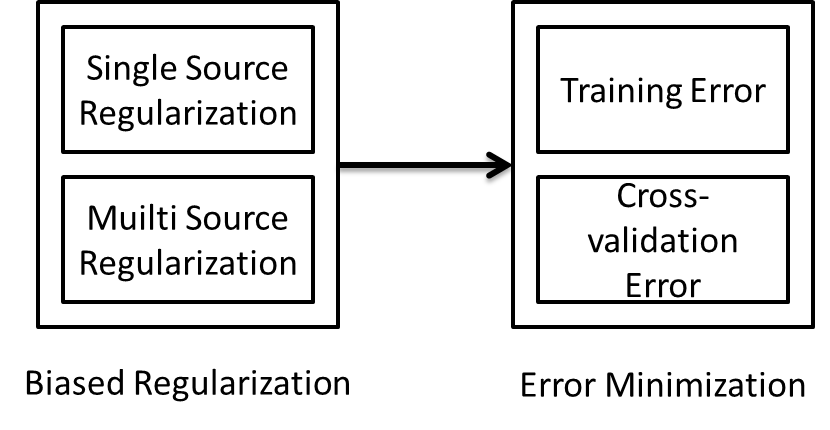
\includegraphics[scale =1]{relatedwork/fig/parameters.png}
	\caption{Two steps for parameter transfer learning. In the first step multi-source and single source combination are usually used to generate the regularazation term. The hyperplane for the transfer model can be obtained by either minimizing training error or cross-validation error on the target training data.}
\end{figure}
\begin{itemize}
	\item Regularization framework: In the regularization framework, some researchers propose to transfer the parameters of the SVM following the assumption that the hyperplane for the target task should be related to the hyperplane of the source models. Evgeniou et al. \cite{evgeniou2004regularized} propose an idea that the hyperplane of the SVM for the target task should be separate into two terms: a common term shared over tasks and a specific term related to the individual task. Inspired by this idea, some researchers propose different strategies to combine these two terms for transfer learning \cite{aytar2011tabula} \cite{tommasi2010safety} \cite{yang2007cross}. Most of these work contains two steps. In the first step, a SVM objective function with a biased regularization term for the target model is build. Then another objective function is build to reduce the empirical error of the target model on the target data.
	\item Neural network framework. In neural network framework, the idea is to use the parameters of a CNN pre-trained from a very large dataset as an initialization to reduce the bias when the target data is small. Yosinski et al. \cite{yosinski2014transferable} show that the high level layer parameters are more related to a specific task while the low level layer ones are more general and transferable. This framework is widely used for image recognition task. By re-using and fine-tuning the parameters of some layers in the pre-trained model, the bias of the target task can be greatly alleviated \cite{Chatfield14} \cite{hoffman2013one}  \cite{zeiler2014visualizing} \cite{NIPS2014_Zhou}. 
	\item Bayesian framework. In Bayesian framework, one or several posterior probabilities of the source data or parameters of the source model can be used to generate a prior probability for the target task. With this prior probability, a posterior probability for the target task can be obtained with the target data.
	Li et al. \cite{fei2006one} use a prior probability density function to model the knowledge from the source and modify it with the data from target to generate posterior density for detection and recognition. 
	Rosenstein et al. \cite{rosenstein2005transfer} use hierarchical Bayesian method to estimate the posterior distribution for all the parameters and the overall model can decide the similarities of the source and target tasks. 
\end{itemize}


\subsection{Avoid Negative Transfer}
In transfer learning, for a given target task, the performance of a transfer method depends on two aspects: the quality of the source task and the transfer ability of the transfer algorithm. The quality of the source task refers to how the source and target tasks are related. If there exists a strong relationship between the source and target, with a proper transfer method, the performance in the target task can be significantly improved. However, if the source and target tasks are not sufficiently related, despite of the transfer ability of the transfer algorithm, the performance in the target task may fail to be improved or even decrease. In transfer learning, negative transfer refers to the degraded performance compare to a method without using any knowledge from the source \cite{pan2010survey}. 
For example, we can use a teacher-student diagram to illustrate the procedure of transfer learning. The student (target model) would like to learn the new knowledge (target task) with the assistance of a teacher (source knowledge). If the teacher can provide helpful knowledge (related knowledge), the student can learn the new knowledge very quickly (positive transfer). If the teacher can only provide useless knowledge, the student could not learn the new knowledge effectively or even get confused (negative transfer).

\begin{figure}
\centering
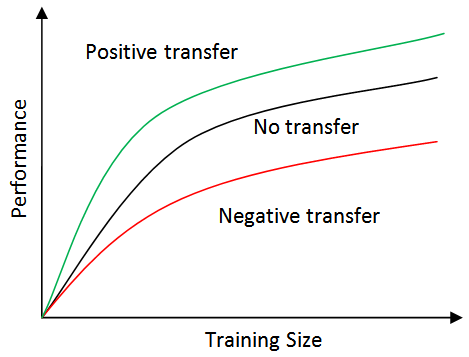
\includegraphics[scale=.7]{relatedwork/fig/negative.png}
\caption{Positive transfer VS Negative transfer.}
\end{figure}

Another important aspect that affect the learning performance is the transfer ability of the algorithm used for the target task. An ideal transfer algorithm would be able to produce positive transfer on related tasks while avoiding negative transfer on unrelated tasks. However, in practice, it is not easy to achieve these two goals simultaneously. Approaches that can avoid negative transfer often bring some affects on positive transfer due to their caution. On the other hand, approaches using aggressive transfer strategies often have little or no protection against negative transfer \cite{torrey2009transfer}. Even though voiding negative transfer is an important issue in transfer learning, how to avoid negative transfer has not been widely addressed \cite{lu2015transfer} \cite{pan2010survey}. Previous work show suggest that negative transfer can be alleviated through 3 approaches \cite{torrey2009transfer}: 
\begin{itemize}
	\item Rejecting unrelated source information. A important approach to avoid negative transfer is to recognize and reject unrelated and harmful source knowledge. The goal of this approach is to minimize the impact of the unrelated source, so that the transfer model performs no worse than the learned model without transfer. Therefore, in some extreme situation, the transfer model is allowed to completely ignore the source knowledge. 
		Torrey et al. \cite{torrey2005using} propose a method using advice-taking algorithm to reject the unrelated source knowledge. 
		Rosenstein et al. \cite{rosenstein2005transfer} present an approach that use naive Bayes classifier to detect and reject the unrelated source.
	\item Choosing correct source task. When the source knowledge come from more than one candidate source, it is possible for the transfer model to select the best source knowledge of the candidates. In this scenario, leverage the knowledge from the best candidate may be effective against negative transfer as long as the best source knowledge is sufficiently related. 
		Talvitie et al. \cite{talvitie2007experts} propose a method that can iteratively evaluate the candidate sources through a trail-and-error approach and select the best one to transfer. Kuhlmann et al. \cite{kuhlmann2007graph} construct a kernel function from certain sources for the target task by estimating the bias from a set of candidate sources whose relationship to the target task is unknown.
	\item Measuring task similarity. To achieve a better transfer performance, it is reasonable for a transfer method to transfer the knowledge from multiple sources instead of just choosing a single source. In this approach, some methods try to involve all the source knowledge without considering the explicit relationship between the source and target. The other methods try to model the relationships between the source and target tasks and use the information as a part of their transfer methods which can significantly reduce the affect of negative transfer.
		 Bakker et al. \cite{bakker2003task} propose a method to provide guidance on how to avoid negative transfer by using clustering and Bayesian approach to estimate the similarities between the target task and multiple source tasks.
		 Tommasi et al. \cite{tommasi2014learning} construct the transfer model by using some transfer parameters to measure the relationships between each source and the target tasks and the transfer parameters are optimized by minimizing the cross-validation error of the transfer model. Similar approaches can be found in \cite{jie2011multiclass} \cite{kuzborskij2013n}.
		 Kuzborskij et al. \cite{kuzborskij2013stability} provide some theoretical analysis of transfer learning and show that regularized least square SVM with truncation function and leave-one-out cross-validation for source task measurement can reduce negative transfer even though the training data of the target task is relatively small.
\end{itemize}

Here we can see that most of the previous approaches focus on measuring the similarity of the source and target tasks, i.e. try to assign the most related source tasks to the target one through various of metrics and use aggressive transfer algorithm to exploit the source knowledge. Just a few work \cite{tommasi2010safety} \cite{kuzborskij2013stability} addressed the problem that a sophisticated transfer algorithm should be designed to better exploit the source knowledge as well as avoid negative transfer. Therefore, in this thesis, we mainly focus on how to design a better transfer algorithm for transfer learning while certain source knowledge is assigned. 

To summarize, in this section, we reviewed 3 types of inductive transfer learning approaches and discussed how to avoid the negative transfer in transfer learning. In our problem, as we have the assumption that the source data is access prohibited, we are not able to use instance transfer and feature transfer approaches. Therefore, we propose a transfer method based on parameter transfer approach. To reduce the affect negative transfer, in our transfer method, we adopt several ideas from the work mentioned above. 



\section{Summary}
In this chapter, we reviewed the some concepts and work related to this thesis. We demonstrate the main methods related to our work and their limitations. In the following chapters, we will provide the technical details of this thesis. 
\chapter{Learning Single Source Categories}
In this chapter, we study the problem that transfer the knowledge from a single source to recognize single source self-defined categories. As we mentioned in Chapter \ref{sec:intro}, we defined two kinds of self-defined categories: single-source and multi-source self-defined categories. We first introduce our strategy to handle single source categories and the multi-source can be solved using the similar strategy.

To deal with this problem, we firstly propose a data argumentation strategy for single source category. We use the transfer parameters to control the amount of knowledge transferred from the source. To estimate the transfer parameters, we propose a novel objective function that be solved effectively and avoid negative transfer. With extensive experiments on the public benchmark MNIST, we empirically show that our method can effectively transfer the knowledge from a single source and avoid negative transfer while other benchmark transfer methods suffer.

\hl{The rest of this chapter is organized as follow:}
\section{Issues in Transfer Learning} 
The motivation of transfer knowledge between different domains is to apply the previous information from the source domain to the target one, assuming that there exists certain relationship, explicit or implicit, between the  feature space of these two domains \cite{pan2010survey}. Technically, previous work can be concluded into solving the following three issues: what, how and when to transfer \cite{tommasi2014learning}.


\textbf{What to transfer.} Previous work tried to answer this question from three different aspects: selecting transferable instances, learning transferable feature representations and transferable model parameters. Instance-based transfer learning assume that part of the instances in the source domain could be re-used to benefit the learning for the target domain. Lim et al. proposed a method of augmenting the training data by borrowing data from other classes for object detection \cite{lim2012transfer}. Learning transferable features means to learn common feature that can alleviate the bias of data distribution in target domain. Recently, Long et al. proposed a method that can learn transferable features with deep neural network and showed some impressive results on the  benchmarks \cite{LongICML15}. Parameter transfer
approach assumes that the parameters of the model for the source task can be transfered to the target task. Yang et al. proposed Adaptive SVMs by transferring parameters by incorporating the auxiliary classifier trained from source domain \cite{yang2007cross}. On top of Yang's work, Ayatar et al. proposed PMT-SVM that can determine the transfer regularizer according to the target data automatically \cite{aytar2011tabula}. Tommasi et al. proposed Multi-KT that can utilize the parameters from multiple source models for the target classes  \cite{tommasi2014learning}.
Kuzborskij et al. proposed a similar method to learn new categories by leveraging over the known source \cite{kuzborskij2013n}.

\textbf{When and how to transfer.} The question \textit{when to transfer} arises when we want to know if the information acquired from previous task is relevant to the new one (i.e. in what situation, knowledge should not be transfered). 
\textit{How to transfer} the prior knowledge effectively should be carefully designed to prevent inefficient and negative transfer. Some previous work consists in using generative probabilistic method \cite{davis2009deep} \cite{wang2014active} \cite{zhou2014multi}.  Bayesian learning methods can predict the target domain by combining the prior source distribution to generate a posterior distribution. Alternatively, some previous max margin methods show that it is possible to learn from a few examples by minimizing the  Leave-One-Out (LOO) error for the training model \cite{kuzborskij2013n} \cite{tommasi2010safety}. Previous work shows that there is a closed-form implementation of LOO cross-validation that can generate unbiased model estimation for LS-SVM \cite{cawley2006leave}.

\hl{Our work correspond to the context above. In this chapter, I propose SMITLe based on parameter transfer approach with LS-SVM. I address my work on how to prevent negative transfer when the source data is not accessible. Compared to other works, I propose a novel strongly convex objective function for transfer parameters estimation. I show that SMITLe can converge at the rate of $O(\frac{\log(t)}{t})$. 
By optimizing this objective function, SMITLe can autonomously adjust the transfer parameters for different prior knowledge. I theoretically and empirically show that, without any data distribution assumption, the superior bound of the training loss for SMITLe is the loss of a method learning directly (i.e. without using any prior knowledge). Experiment results show that when the prior knowledge hurts the transfer procedure, SMITLe can avoid negative transfer by ignoring the unrelated prior knowledge autonomously. Extensive experiments also show that when the prior knowledge is very related (positive transfer), my method can outperform other methods by exploiting the prior knowledge greatly.}

\section{Related Work}\label{sec:single:rl}
In this part, We will introduce the framework my work based on and some related previous work. We first introduce the basic principle of LS-SVM. Based on LS-SVM, several transfer methods are introduced, including A-SVM, PMT-SVM, Multi-KT and MULTIpLe. In these methods, the first two can only adopt the knowledge from single source model and the rest can adopt the knowledge from multiple ones.
\subsection{LS-SVM Classifier}
Least Square SVM is proposed is least squares versions of support vector machines (SVM), which are a set of related supervised learning methods that analyze data and recognize patterns \cite{suykens1999least}. By replacing the hinge loss in classical SVM with L2 loss, LS-SVM classifier is obtained by reformulating the minimization problem as: 
\begin{equation}\label{eq:gama:lssvm}
\begin{aligned}
\min \qquad& L_{LSSVM} = \frac{1}{2}{\left\| w \right\|^2} + \frac{C}{2}\sum\limits_{i = 1}^l {{\varepsilon_i ^2}}\\
\text{s.t.}\qquad&{y_i} = w{x_i} + b + {\varepsilon _i} \quad   \text{for} \quad i \in \left\{ {1,2,...,l} \right\}
\end{aligned}
\end{equation}

The primal Lagrangian for this optimization problem given the unconstrained minimization problem can be written as:
\begin{equation}\label{sq:gama:lsprime}
  L\left( {w,b,\alpha ,\varepsilon } \right) = \frac{1}{2}{\left\| w \right\|^2} + \frac{C}{2}\sum\limits_{i = 1}^l {{\varepsilon _i}^2}  - \sum\limits_{i = 1}^l {{\alpha _i}\left\{ {w{x_i} + b + {\varepsilon _i} - {y_i}} \right\}}
\end{equation}

Where $\alpha = [ \alpha_1,...,\alpha_l]^T $ is the vector of Lagrange multipliers. The solution to minimise this problem is give by:
\begin{equation}
  \left[ {\begin{array}{*{20}{c}}
{K  + \frac{1}{C}{\rm I}}\\
1^T
\end{array}\begin{array}{*{20}{c}}
1\\
0
\end{array}} \right]\left[ {\begin{array}{*{20}{c}}
\alpha \\
b
\end{array}} \right] = \left[ \begin{array}{l}
y\\
0
\end{array} \right]
\end{equation}
Where $K \in R^{l \times l},K_{i,j}=x_i \times x_j^T$. $I$ is the identity matrix and $\mathbf{1}$ is a column vector with all its elements equal to 1. With:
\begin{equation}\label{eq:gama:psi}
\psi^{-1} = \left[ {\begin{array}{*{20}{c}}
{K  + \frac{1}{C}{\rm I}}\\
1^T
\end{array}\begin{array}{*{20}{c}}
1\\
0
\end{array}} \right]^{-1}
\end{equation}
Problem \eqref{sq:gama:lsprime} can be solved by:
\begin{equation}
\left[ {\begin{array}{*{20}{c}}
\alpha \\
b
\end{array}} \right] = \psi^{-1}\left[ \begin{array}{l}
y\\
0
\end{array} \right]
\end{equation}
\subsection{ASVM \& PMT-SVM}
Adaptive SVM (ASVM) is the first work using LS-SVM for transfer learning for vision related tasks \cite{yang2007adapting}. The goal of ASVM is to minimize the distance between the target hyperplane $w$ and source one $w'$ incorporating with the transfer parameter $\gamma$. The objective function is defined as follow:
\begin{equation}\label{eq:gama:asvm}
\begin{aligned}
\min \qquad& L_{ASVM} = \frac{1}{2}{\left\| w - \gamma w' \right\|^2} + \frac{C}{2}\sum\limits_{i = 1}^l {{\varepsilon_i ^2}}\\
\text{s.t.}\qquad&{y_i} = w{x_i} + b + {\varepsilon _i} \quad   \text{for} \quad i \in \left\{ {1,2,...,l} \right\}
\end{aligned}
\end{equation}

Here, $\gamma$ controls the amount of transfer regularization. Intuitively, the regularization term of ASVM is like a spring between $w$ and $\gamma w'$. Equivalently, assume ${\left\| {w'} \right\|^2}=1$ and the regularization term can be expended as:
\begin{equation*}
{\left\| {w - \gamma w'} \right\|^2} = {\left\| w \right\|^2} - 2\gamma \left\| w \right\|\cos \theta  + {\gamma ^2}
\end{equation*}
Where $\theta$ is the angel between $w$ and $w'$. However, the term $-\gamma \left\| w \right\|\cos \theta$ also encourages $||w||$
to be larger (as this reduces the cost) which prevents margin maximization. Thus $\gamma$, which defines the amount of transfer regularization, becomes a tradeoff parameter between margin maximization and knowledge transfer.
\begin{figure}
\centering
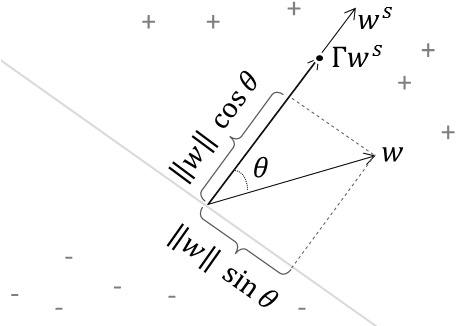
\includegraphics[scale=.6]{transfer/fig/pmt-svm.png}
\caption{Projecting $w$ to $w'$ in PMT-SVM (adapted from \cite{aytar2011tabula}).}\label{fig:gama:pmt}
\end{figure}

Based on this, Projective Model Transfer SVM (PMT-SVM) is proposed to solve the transfer problem by optimizing the following objective function \cite{aytar2011tabula}:
\begin{equation}\label{eq:gama:pmt}
\begin{aligned}
\min \qquad& {L_{PMT}} = \frac{1}{2}{\left\| w \right\|^2} + \gamma {\left\| {Pw'} \right\|^2} + \frac{C}{2}\sum\limits_{i = 1}^l {\varepsilon _i^2} \\
\text{s.t.}\qquad&{y_i} = w{x_i} + b + {\varepsilon _i} \quad   \text{for} \quad i \in \left\{ {1,2,...,l} \right\}\\
& w^Tw' \ge 0
\end{aligned}
\end{equation}

Where $P$ is the the projection matrix $P = I - \frac{{w{'^T} \times w'}}{{w' \times w{'^T}}}$. Therefore, ${\left\| {Pw} \right\|^2} = {\left\| w \right\|^2}{\sin ^2}\theta $ is the
squared norm of the projection of the $w$ onto the source hyperplane (see Figure \ref{fig:gama:pmt}). As $\gamma \rightarrow 0$, the loss function \eqref{eq:gama:pmt} becomes a classic LS-SVM loss function. Because \eqref{eq:gama:pmt} is convex, it can be solved effectively by quadratic optimization.

In summary, both ASVM and PMT-SVM are designed to answer the question: how to transfer by solving some convex objective function. However, they both require a pre-defined parameter $\gamma$, which controls the amount of the knowledge to be transfered, to complete the objective function. In most cases, this parameter can only be set according to the background knowledge. Also, both methods can only adopt the knowledge from single source model which limits the their performance. 
\subsection{Multi-KT}
To learning from many sources, Multi Model Knowledge Transfer (Multi-KT) is proposed to reply on multiple sources by assigning different weight for each of them \cite{tommasi2014learning}. Similar to the objective function \eqref{eq:gama:asvm}, its objective function is defined as follow: 
\begin{equation}\label{eq:gama:multi}
\begin{aligned}
\min \qquad& {L_{Multi - KT}} = \frac{1}{2}{\left\| {w - \sum\limits_k {{\beta _k}} {{w'}_k}} \right\|^2} + \frac{C}{2}\sum\limits_{i = 1}^l {{\zeta _i}\varepsilon _i^2}  \\
\text{s.t.}\qquad&{y_i} = w{x_i} + b + {\varepsilon _i} \quad   \text{for} \quad i \in \left\{ {1,2,...,l} \right\}
\end{aligned}
\end{equation}
Here, $\beta_k$ is the weight assigned for the $k$th source model and $\zeta _i$ is defined as:
\begin{equation*}
{\zeta _i} = \left\{ {\begin{array}{*{20}{c}}
{\frac{N}{{2{N^ + }}}}&{{\text{if }}{y_i} =1}\\
{\frac{N}{{2{N^ - }}}}&{{\text{if }}{y_i} =- 1}
\end{array}} \right.
\end{equation*}
where $N^+$ and $N^-$ are number of positive and negative examples respectively and $N$ is the total number of examples. 

The primal Lagrangian for optimization problem \eqref{eq:gama:multi} can be written as:
\begin{equation}
{L_{Multi - KT}}\left( {w,\beta ,\varepsilon ,\alpha } \right) = \frac{1}{2}{\left\| {w - \sum\limits_k {{\beta _k}} {{w'}_k}} \right\|^2} + \frac{C}{2}\sum\limits_{i = 1}^l {{\zeta _i}\varepsilon _i^2}  + \sum\limits_{i = 1}^l {{\alpha _i}\left[ {w{x_i} + b + {\varepsilon _i} - {y_i}} \right]} 
\end{equation}
So problem \eqref{eq:gama:multi} can be solved once $\beta$ is set.
Different from ASVM and PMT-SVM which require background knowledge to select proper transfer parameter, Multi-KT can estimate the transfer parameter $\beta$ itself by using the closed-form Leave-One-Out (LOO) error. According to \cite{cawley2006leave}, the closed-form LOO error is defined as:
\begin{equation}\label{eq:gama:loo}
{y_{i}} - {\hat y_{i}} = \frac{{{\alpha _{i}}}}{{\psi_{ii}^{ - 1}}}{\qquad\text{for}}\qquad i = 1,...,l
\end{equation}
Here $\psi_{ii}^{-1}$ is its $ith$ diagonal element of $\psi^{-1}$ in \eqref{eq:gama:psi}.

To estimate $\beta$, a loss function, similar to hinge loss, is defined as: 
\begin{equation}\label{eq:gama:multib}
\begin{aligned}
\text{min} \qquad&{\cal L} = \sum\limits_i^l {{\zeta _i}{{\left| {1 - {y_i}{{\hat y}_i}} \right|}_ + }} \\
\text{s.t.} \qquad& \left\| \beta  \right\| \le 1
\end{aligned}
\end{equation}

Here $|x|_+=max(x,0)$. Intuitively, if $\beta$ is properly set, ${y_i}{{\hat y}_i}$ should be positive for each $i$. However, focusing only on the sign of those quantities would result in a non-convex formulation with many local minima. By adding the $|\cdot|_+$ function, formula \eqref{eq:gama:multib} becomes convex and can be solved by gradient descent method.

\subsection{MULTIpLE}
MULticlass Transfer Incremental LEarning (MULTIpLE) focuses on adding a new class to a existing $N$ class source problem while preserving the performance on the old classes \cite{kuzborskij2013n}. To preserving the overall performance of the classifier among $N+1$ classes, MULTIpLE contains two parts: incremental learning for existing $N$ classes and transfer learning for the new class.

For the existing $N$ classes, MULTIpLE uses the similar strategy as ASVM, setting the transfer parameter $\gamma$ to 1. For the new class, it adopts the strategy of Multi-KT, combining knowledge from existing $N$-class models. As a result, the objective function for the hyperplanes in MULTIpLE is defined as:
\begin{equation}
\begin{aligned}
\text{min}\qquad {} & L_{MULTIpLE}=\frac{1}{2}\sum\limits_{n = 1}^N {{{\left\| {{w_n} - {{w'}_n}} \right\|}^2}}  + \frac{1}{2}{\left\| {{w_{N + 1}} - \sum\limits_{k = 1}^N {w{'_k}{\beta _k}} } \right\|^2}+ \frac{C}{2}\sum\limits_{n = 1}^{N + 1} {\sum\limits_{i = 1}^l {\varepsilon _{i,n}^2} }  \\
\text{s.t.}\qquad {} &{\varepsilon _{i,n}} = {Y_{in}} -  {x_i}{w_n} - {b_n}
\end{aligned}\label{eq:gama:multiple}
\end{equation}

Similar like Multi-KT, MULTIpLE uses LOO error in \eqref{eq:gama:loo} to estimate the transfer parameter $\beta$ for the new class. The objective function for $\beta$ estimation is defined by \cite{crammer2002algorithmic}:
\begin{equation}\label{eq:gama:multib}
\begin{aligned}
\text{min} \qquad& {\cal L}\left( {\beta ,i} \right) = \left\{ {\begin{array}{*{20}{c}}
{\mathop {\max }\limits_{n \ne {y_i}} {{\left| {1 - {{\hat Y}_{in}}\left( \beta  \right) - {{\hat Y}_{i{y_i}}}\left( \beta  \right)} \right|}_ + }}&{{:y_i} \ne N + 1}\\
{\left| {1 - {{\hat Y}_{in}}\left( \beta  \right) - {{\hat Y}_{i{y_i}}}\left( \beta  \right)} \right|}&{{:y_i} = N + 1}
\end{array}} \right.  \\
\text{s.t.} \qquad& \left\| \beta  \right\| \le 1
\end{aligned}
\end{equation}
We can find the optimal $\beta$ with projected subgradient descent \cite{BoydCO}. 
\section{Linear Combination Strategy}\label{sec:single:comb}
A major challenge in transferring the knowledge from the source is to design a strategy to combine the source knowledge with the knowledge from the target task. In this section, we propose propose a combination strategy that using linear combination to combine the source and target knowledge. An important advantage of this strategy is that we can adjust the impact of the knowledge comes from the source model more flexibly by just modifying the value of its coefficient. As long as the source knowledge hurts the transfer model, we can reduce its impact to avoid negative transfer.

\hl{Intuitively}, when transferring the knowledge from another task, the performance of the model for the target task is greatly determined by the relationship of these two tasks. Here we use the $\mathcal{H}$-divergence to measure the relationship of two different tasks. $\mathcal{H}$-divergence can be defined as follow:
\begin{definition}
	(from Kifer et al. \cite{kifer2004detecting}) Given a domain $\mathcal{X}$ with two probability distributions, let $\mathcal{H}$ be a hypothesis class on $\mathcal{X}$ and denote by $I(h)$ the set for which $h \in \mathcal{H}$ is the characteristic function where $x\in I(h) \leftrightarrow h(x)=1$. The $\mathcal{H}$-divergence between these two probability distribution $D$ and $D'$ is 
	\begin{equation*}
	{d_{\mathcal{H}}}\left( {D,D'} \right) = 2\mathop {\sup }\limits_{h \in {\mathcal{H}}} \left| {{{\Pr }_D}\left[ {I(h)} \right] - {{\Pr }_{D'}}\left[ {I(h)} \right]} \right|
	\end{equation*}
\end{definition}
When $D$ and $D'$ are related, $d_{\mathcal{H}}\left( {D,D'} \right)$ is small and $d_{\mathcal{H}}\left( {D,D'} \right)$ is large when they are unrelated. Ben et al. \cite{ben2010theory} show that the performance of the target model is affected by the $\mathcal{H}$-divergence of the probability distributions of the two tasks. 

Then our single source self-defined category problem can be described as follow: Given a task  $T$ to distinguish whether an example is from one certain category $C$ from a domain $\mathcal{X} \times \mathcal{Y}$ with $D$ probability distribution over $\mathcal{X}$, $\mathcal{X}$ is the input feature and $\mathcal{Y}$ is the label set $\{1,-1\}$. We use an examples with label 1 to denote the positive example (i.e. belongs to the category) and an example with label -1 to denote the negative example (i.e. not belong to the category). We assume that we have another source model $f'$ trained from another independent task $S$ on another domain $\mathcal{X'} \times \mathcal{Y'}$ with $D'$ probability distribution over $\mathcal{X'}$ and $S$ and $T$ are related. We assume that a small training set $T_{train}=\{(x,y)\} \subset \mathcal{X}\times \mathcal{Y}$, $\mathcal{X}$ is given. We want to learn a classification problem $f: \mathcal{X} \rightarrow \mathcal{X}$ from $T_{train}$ incorporating with $f'$ so that $f$ can perform well on a independent testing set $T_{test}=\{(x,y)\} \subset \mathcal{X} \times \mathcal{Y}$.

Here, let's set the both source and target model $f$ and $f'$ in the hypothesis space of function $\mathcal{H}$ which equals to space of all the linear models of the form. 
\begin{equation}
f(x)=w^Tx+b
\end{equation}
%where $\phi(x)$ is a feature mapping that maps the input space into a another high or even possible infinite dimensional space.

To leverage the knowledge from the source model $f'$, we propose a method where a part of the decision of the target model $f$ comes from the decision of the source model $f'$. This process can be written as:
\begin{equation}\label{eq:single:linear}
\begin{aligned}
 f(x) = & w^T\phi(x)+b+\gamma f'(x) \\
\text{st.} \qquad & f'(x) = w'^T\phi(x)
\end{aligned}
\end{equation}

\begin{figure}
	\centering
	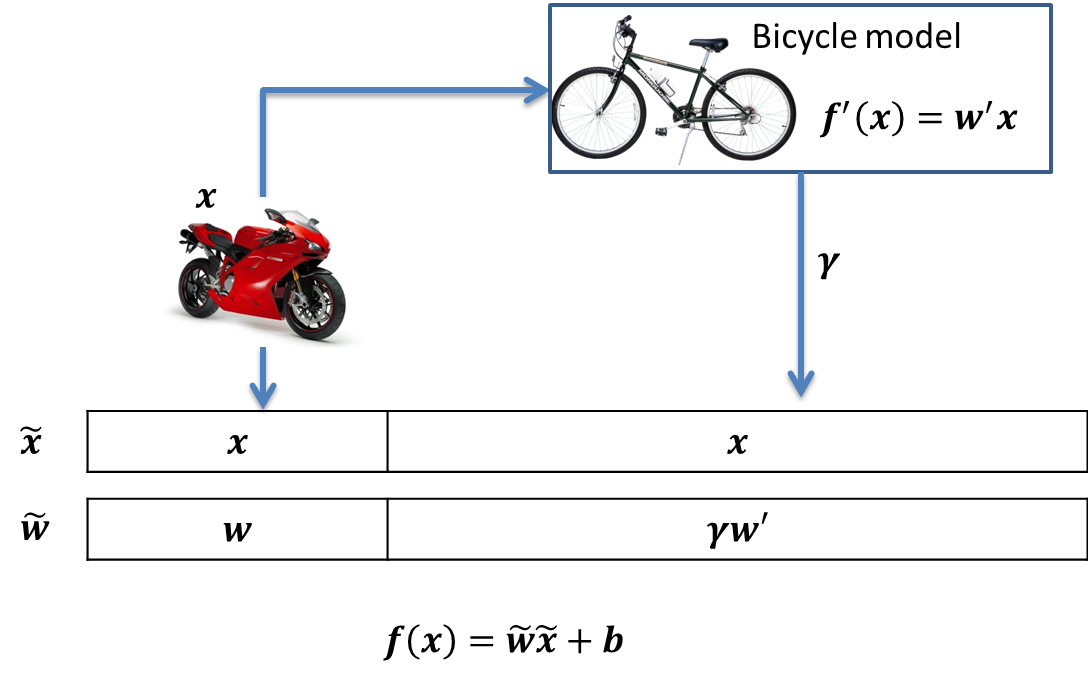
\includegraphics[scale=.6]{transfer/fig/argumentation.png}
	\caption{A graphical representation of linear combination. The score from the source model can be considered as an auxiliary feature and the transfer parameter controls the value of the auxiliary feature.}\label{fig:single:arg}
\end{figure}
Where $\gamma$ is called the transfer parameter $\gamma$ that controls the amount of the knowledge transferred from the source model $f'$. 
While combining the knowledge linearly, we can have several advantages especially when we use linear model such as SVM.

The first advantage is simplicity. Given a example $x$ and a source model $f'$, to consider the decision from the source model, we can simply add its score $f'(x)$ in to affect the decision of the target model. It is equivalent to the data argumentation approach where the score of the source model is used as the auxiliary feature (see Figure \ref{fig:single:arg}). Accordingly, the extra dimension which is set to 1, is added into the hyperplane $w$. By introducing the auxiliary information from the source model, we expect to reduce the bias from the target training set. As a result, we can successfully transfer a transfer learning problem into a traditional machine learning problem with data argumentation.  
Another advantage is flexibility. By using the transfer parameter to control the amount of the knowledge from the source model, the model for the target task is more adaptive to various of situation. Previous work  \cite{kuzborskij2013n} \cite{tommasi2014learning} just consider two situations: unrelated source and positive correlated source. Here we add another situation negative correlated source and expand the previous situation into 3:
\begin{itemize}
	\item When the two tasks are not related, it is expected to get a random score from the source model and the transfer parameter should be set to 0 to ignore it. Therefore, the target model won't affected by the noisy dimension and is less likely to suffer from negative transfer. In the extreme case where the transfer parameter is set 0, no auxiliary information is introduced to the target task and therefore, we can guarantee that, at least, negative transfer won't happen.
	\item When the source and target tasks are positive correlated, i.e. for a positive example $x_p$ and a negative example $x_n$, we have $f'(x_p)>f'(x_n)$, we expect the transfer parameter to be positive. Therefore, the positive and negative examples are more distinct and can be better distinguished by the hyperplane.
	\item  For the same reason above, we expect the transfer parameter to be negative if the two tasks are negative correlated.
\end{itemize}

Therefore, let $\tilde{x} = (x,x)$ and $\tilde{w} = (w,\gamma w')$.
With the LS-SVM setting, our transfer problem can be solved by solving the following optimization problem with argument data:
\begin{equation}\label{eq:single:reg}
	\begin{aligned}
	\min \qquad& L_{LSSVM}(\tilde{w}) = \frac{1}{2}{\left\| \tilde{w} \right\|^2} + \frac{C}{2}\sum\limits_{i = 1}^l {{e_i ^2}}\\
	\text{s.t.}\qquad& \tilde{w} = (w,\gamma w')\\
	&{y_i} = \tilde{w} {\tilde{x_i}} + b + {e _i} \quad   \text{for} \quad i \in \left\{ {1,2,...,l} \right\}\\
	\end{aligned}
\end{equation}
When we consider the transfer parameter $\gamma$ as a constant that can be determined by certain prior knowledge, to regularize  $\left\|\tilde{w}\right\|^2$ is equivalent to regularize $\left\|\tilde{w}-\gamma w'\right\|^2$. Therefore, function \eqref{eq:single:reg} can be represented as:
\begin{equation}\label{eq:single:formreg}
\begin{aligned}
\min \qquad& L_{\gamma}(w) = \frac{1}{2}{\left\| {w}-\gamma w' \right\|^2} + \frac{C}{2}\sum\limits_{i = 1}^l {{e_i ^2}}\\
\text{s.t.}\qquad& {y_i} = {w} {{x_i}} + b + {e _i} \quad   \text{for} \quad i \in \left\{ {1,2,...,l} \right\}\\
\end{aligned}
\end{equation}

To solve the problem \eqref{eq:single:formreg}, we first introduce some important notations used in the rest of this chapter in Table \ref{tab:single:notation}. We use any letter with apostrophe to denote the information from the source data, e.g. if $f(x)$ denotes the model for the target task, $f'(x)$ denotes the model for the source one.

% Table generated by Excel2LaTeX from sheet 'Sheet1'
\begin{table}
	\centering
	\caption{\hl{Notations used in this chapter}}
	\begin{tabular}{|c|L{14cm}|}
		\hline
		$f'(x)$ & binary model for source task \\
		\hline
		$f(x)$  & binary model for target task \\
		\hline
		$\phi(x)$ &  function mapping the input sample into a high dimensional feature space. \\ \hline
		%    $K(x,x)$ & kernel matrix with  $\phi(x_i) \cdot\phi(x_j)$ corresponding to its element $(i,j)$\\ \hline
		$X$     & instance matrix with each row representing one instance \\\hline
		$\boldsymbol{W} $    & (N+1)-column hyperplane matrix for target task. Each column represents one hyperplane of a binary model \\\hline
		$\boldsymbol{W'}$    & hyperplane matrix for the source task \\\hline
		$\boldsymbol{a'} $   & the Lagrangian multiplier matrix for source problem. Each column represents a set of Lagrangian multiplier for a binary SVM model \\\hline
		$\boldsymbol{a} $    & the Lagrangian multiplier matrix for target problem \\
		\hline
		$\boldsymbol{b'},\boldsymbol{b}$  & the bias vector for source and target task \\
		\hline
		$\boldsymbol{a_i}$ & $i_{th}$ column of matrix $\boldsymbol{a}$ \\ \hline
		%    $d_\gamma$ &  diagonal matrix with$\left[ {{\gamma _1},...,{\gamma _N}} \right]$ in its main diagonal\\\hline
		$\boldsymbol{\beta}$ & row vector $\left[ {{\beta _1},...,{\beta _N}} \right]$ to control the prior knowledge for the new category\\ \hline
		$\varepsilon_{ny_i}$&loss parameter. $\varepsilon _{n{y_i}}=1$ if $n=y_i$ and 0 otherwise\\ \hline
		$\psi$, $\psi^{-1}$ & $\psi$ is the modified kernel matrix for solving binary LS-SVM and $\psi^{-1}$ is the inverse matrix of $\psi$\\ \hline
	\end{tabular}%
	\label{tab:single:notation}%
\end{table}%

The primal Lagrangian for this optimization problem \ref{eq:single:formreg} given the unconstrained minimization problem can be written as: 
\begin{equation}
	{L_\gamma }\left( {w,b,\alpha ,e} \right) = \frac{1}{2}{\left\| {w - \gamma w'} \right\|^2} + \frac{C}{2}\sum\limits_{i = 1}^l {{e _i}^2}  - \sum\limits_{i = 1}^l {{\alpha _i}\left\{ {w{x_i} + b + {e_i} - {y_i}} \right\}} 
\end{equation}
The optimal solution can be found by satisfying the following condition:
\begin{eqnarray}\label{eq:single:lssvm-deriv}
\begin{aligned}
\frac{{\partial L}}{{\partial w}} = 0 &\to w = \gamma w' + \sum\limits_i^l {{\alpha _i}{x_i}} \\
\frac{{\partial L}}{{\partial b}} = 0 &\to \sum\limits_i^l {{\alpha _i} = 0} \\
\frac{{\partial L}}{{\partial e_i}} = 0 &\to C{e_i} = {\alpha _i} \qquad i = 1,...,l\\
\frac{{\partial L}}{{\partial {\alpha _i}}} = 0 &\to {y_i} = {w} {{x_i}} + b + {e _i}\qquad i = 1,...,l\\
\end{aligned}
\end{eqnarray}

Let $X=\left[x_1,x_2,...,x_l\right]$ and $Y=[y_1,y_2,...,y_l]$, Eq \eqref{eq:single:lssvm-deriv} can be written in the following compact format:

\begin{equation}\label{eq:single:matrixsolve}
	\left[\begin{array}{cccc}
	\mathbf{I}&0&0&-X^T\\
	0&0&0&-Y^T\\
	0&0&C\mathbf{I}&-I\\
	X&Y&I&0
	\end{array}\right]
	\left[\begin{array}{c}w-\gamma w'\\b\\e\\\alpha
	\end{array}\right]	= \left[\begin{array}{c}0\\0\\0\\\mathbf{1}
	\end{array}\right]
\end{equation} 
where $\mathbf{I}$ is an identity matrix and $\mathbf{1}$ is a column  vector whose elements are 1. 

In real applications, when we have $n$ single source categories and their corresponding source model $f'_1(x),f'_2(x),...,f_n(x)$, their loss function can be represented as:

\begin{equation}\label{eq:single:unionreg}
\begin{aligned}
\min \qquad& L_{\gamma}(w_1,w_2,...,w_n) = \frac{1}{2}\sum\limits_{i = 1}^n{\left\| {w_i}-\gamma_i w_i' \right\|^2} + \frac{C}{2}\sum\limits_{i = 1}^n\sum\limits_{j = 1}^l {{e_{ij} ^2}}\\
\text{s.t.}\qquad& {y_{ij}} = {w_i} {{x_i}} + b_i + {e _{ij}} \quad   \text{for} \quad i \in \left\{ {1,2,...,l}  \right\}, j \in {1,2,...,n}\\
\end{aligned}
\end{equation}
Let $\mathbf{W} = [w_1,w_2,...,w_n]$, $\mathbf{W'} = [w'_1,w'_2,...,w'_n]$ and $D(\gamma)$ be the diagonal matrix $diag(\gamma_1,\gamma_2,...,\gamma_n)$. The corresponding solution for problem \eqref{eq:single:unionreg} is:

\begin{equation}
\left[\begin{array}{cccc}
\mathbf{I}&0&0&-X^T\\
0&0&0&-Y^T\\
0&0&C\mathbf{I}&-I\\
X&Y&I&0
\end{array}\right]
\left[\begin{array}{c}\mathbf{W}- D(\mathbf{\gamma}) \mathbf{W'}\\b\\e\\\alpha
\end{array}\right]	= \left[\begin{array}{c}0\\0\\0\\\mathbf{1}
\end{array}\right]
\end{equation} 
 We can see that Eq. \eqref{eq:single:unionreg} can be solved by directly once the transfer parameters $\gamma=\{\gamma_i|i=1,...,n\}$ is determined.




\section{Cross-Validation Error for LS-SVM}
In this section, we introduce the cross-validation estimation for LS-SVM. As we mentioned in Section \ref{sec:single:comb} that once we determine the value of the transfer parameters $\gamma$, problem \eqref{eq:single:unionreg} can be solved directly. In Section \ref{sec:single:comb}, we treat the transfer parameters as the parameters to be set in advance. In this section, we introduce how we can estimate the unbiased transfer parameters by using an important property of LS-SVM for parameter estimation. 

\subsection{Closed Form Cross-validation Estimation for LS-SVM}
To estimate the transfer parameter, we adopt cross-validation for parameter estimation. Cross-validation is widely used for parameter estimation. Suppose we have a model with one or more unknown parameters, and a data set to which the model can be fit (the dataset). The fitting process optimizes the model parameters to make the model fit the data as well as possible. On the other hand, we have to make sure that this model have the generalization ability, i.e. it can also work well on other independent validation dataset. Otherwise, the model is overfitted to the training data set. However, in practical problem we may not be able to get another independent data set except for the original dataset. Therefore, we have to manually create the validation set by selecting some of the data from the original dataset and use them for evaluation. One round of cross-validation involves partitioning a sample of data into complementary subsets, performing the analysis on one subset (called the training set), and validating the analysis on the other subset (called the validation set or testing set). By repeating these process several rounds with different partitions, we can significant reduce the variability of our estimation using the average results over the rounds.
\begin{figure}
	\centering
	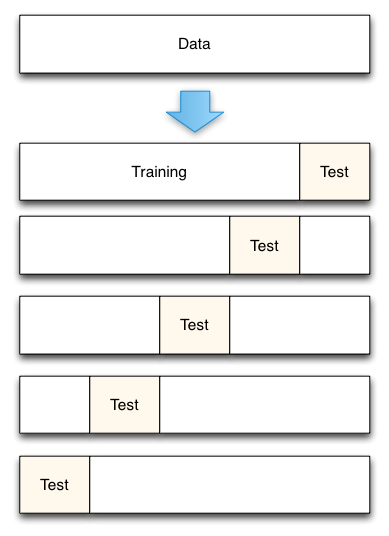
\includegraphics[scale=.4]{transfer/fig/cv.png}
	\caption{An illustration of 5-fold cross-validation}
\end{figure}
There are several different types of cross-validation methods due to their partition strategies. K-fold cross-validation is the most popular type among them. In k-fold cross-validation, the original dataset is randomly partitioned into k equal sized subsamples. K-fold cross-validation is performed in K rounds and in each round, each one of the K partition is used exactly once as the validation set and the rest partitions are used as the training set. 

In our work, we also employ cross-validation for parameter estimation. Here we show that the cross-validation error for LS-SVM can be represented in an efficient way. As a result, we don't have to actually perform cross-validation and re-train the models in each round to obtain the cross-validation error.

\begin{theorem}[An extension of \cite{cawley2006leave}]\label{th:single:cv}
	Given a dataset $D=\{(x_i,y_i)|i=1,...,l\}$, the solution of a LS-SVM on $D$ can be written as Eq. \eqref{eq:gama:lssvm}.
	Assume that $D^{(n)} = \{(x_i,y_i)|i=1,...,n\}$ is a subset of $D$ and $D\backslash D^{(n)}$ is the complement of $D^{(n)}$ in $D$. 
	Let $\left[\alpha_1,...,\alpha_n\right]$ be the corresponding $n$ rows of $\alpha$ in Eq. \eqref{eq:single:orgmatrix} and $S_n$, $s$ and $S_{(l - n + 1)}$ represent the square blocks of matrix:
	
	\begin{equation*}
	\left[ {\begin{array}{c|c}
		{{S_{n }}} &s\\ \hline
		{{s^T}}&{{S_{(l - n + 1)}}}
		\end{array}} \right] =\left[ {\begin{array}{*{20}{c}}
		{K  + \frac{1}{C}{\rm I}}\\
		1^T
		\end{array}\begin{array}{*{20}{c}}
		1\\
		0
		\end{array}} \right]
	\end{equation*}
	The unbiased leave out error of a LS-SVM trained from $D\backslash D^{(n)}$ on $D^{(n)}$ can be estimated as:
	
	\begin{equation*}\label{eq:single:nout}
	ERR_{leave-out} = \left( {{S_n} - sS_{(l - n + 1)}^{ - 1}{s^T}} \right){\left[ {{\alpha _1},...,{\alpha _n}} \right]^T}
	\end{equation*}
\end{theorem}
We show the proof in Appendix \ref{app:cross}. This remarkable result allows cross-validation to be used while only fitting the model once to all available data.

Therefore, we have a convenient solution to estimate the unbiased cross-validation error. However, to perform a cross-validation in practice, decide the partition strategy. Suppose we have $l$ examples in the original data and we want to perform a K-fold cross-validation on it. Thus we have $\mathbf{C^{l/K}_l}$ possible combinations. This means larger K leads to less computation time. Moreover, larger K means less bias towards overestimating the true expected error (as training folds will be closer to the total dataset). When we set $K=l$, we perform $l$-fold cross-validation, i.e. leave-one-out cross-validation (LOO-CV). Vapnik et al. \cite{vapnik2000bounds} show that LOO-CV can provide an almost unbiased estimation error. Previous work also show that transfer learning on the small target training set can be benefit from LOO-CV to better estimate the transfer parameters as well as prevent negative transfer \cite{kuzborskij2013stability}. Due to the reasons above, in this thesis, we use LOO-CV to estimate the transfer parameters to optimize our transfer model.

According to Theorem \ref{th:single:cv}, the LOO-CV error for LS-SVM can be represent as:
\begin{equation}
	ERR_{loo}=\frac{1}{l}\sum_{i}^{l}
\end{equation}
\section{Multi-class Loss with LOO error}
From the previous section we can see that, the unbiased estimated decision value of LOO-CV for an example can be written in a closed form. In this section, we introduce the multi-class loss function and use the LOO-CV error to estimate the multi-class loss. We propose a novel objective function based on the estimated multi-class loss to estimate the transfer parameters.

In previous section, we discussed the LS-SVM in binary class scenario. In practice, we have to handle the multi-class scenario. A common strategy to convert the binary class scenario to a multi-class scenario is to assign label to the highest confidence score of each binary SVM. Suppose we trained $n$ binary SVMs $f_i,i\in 1,...,n$ for a $n$-class problem, the label of an example $x$ is assigned by:
\begin{figure}
	\centering
	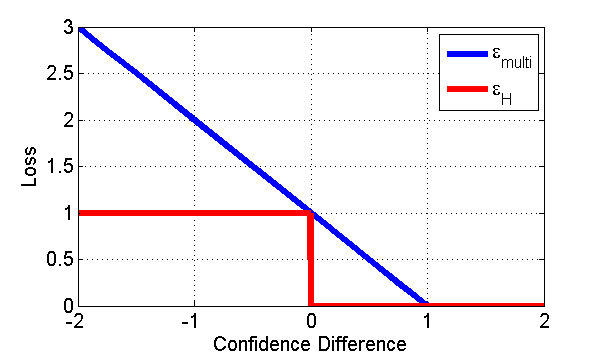
\includegraphics[scale=.7]{transfer/fig/losscmp.png}
	\caption{Loss function comparision for multi-class hinge loss $\epsilon_{multi}$ and classical zero-one loss  $\epsilon_{H}$}\label{fig:single:losscmp}
\end{figure}
\begin{equation}
H_{\mathcal{F}}(x)=\hat{y}=\arg \underset{i \in 1,...,n}{\max}f_i(x)
\end{equation} 
Let $\llbracket y\rrbracket$ be 1 if the predicate $y$ holds and 0 otherwise. The empirical error for a multi-class problem is given by:

\begin{equation} \label{eq:single:discreteloss}
	\epsilon_{H} = \frac{1}{l}\sum_{1}^{l}\llbracket H_{\mathcal{F}}(x_i) \neq y_i \rrbracket
\end{equation}
Our goal is to find a group of function $\mathcal{F}$ that has a small empirical error on the training set as well as on an unforeseen test set. Because function \eqref{eq:single:discreteloss} takes discrete value on the predicate, directly approaches which tries to minimize the empirical error are computational expensive \cite{crammer2002learnability}. Crammer et al. \cite{crammer2002algorithmic} proposed an piecewise linear bound to replace it:

\begin{equation}\label{eq:single:train_loss}
\epsilon _{multi} = \frac{1}{l} \sum_{i}^{l}\epsilon^{(i)} _{multi} =\frac{1}{l} \sum_{i}^{l} \mathop {\max }\limits_{n \in \left\lbrace 1,...,N \right\rbrace } {\left[ {1 - {\varepsilon _{n{y_i}}} + {{f_n(x_i)} - f_{y_i}(x_i)}} \right]}
\end{equation}
where $\varepsilon_{n{y_i}}$ is equal 1 if $n=y_i$ and 0 otherwise. 

According to the multi-class loss \eqref{eq:single:train_loss}, its bound is 0 if the confidence score for the correct label is larger by at least 1 than the confidence scores assigned to the other labels. Otherwise, we suffer a linear loss that is proportional to the difference between the confidence of the correct label and the maximum among the confidence of the other labels (see Figure \ref{fig:single:multi-loss}). 
\begin{figure}
	\centering
	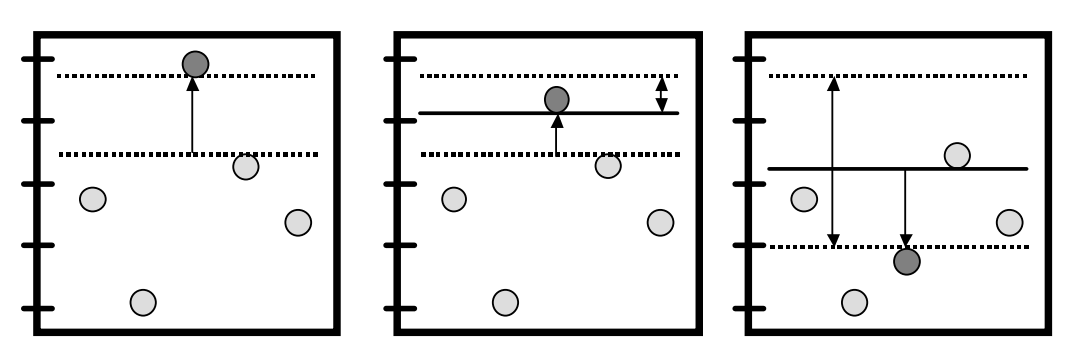
\includegraphics[scale=.5]{transfer/fig/svmloss.png}
	\caption{Illustration of the margin bound for a single example in 3 scenarios. The cirles denote different confidences and the correct label is ploted in dark grey. The height of each lable is the confidence score. In the left figure,$\epsilon(x)=0$. In the middle figure, even though the confidence of the correct label is the largest, it fails to be larger by 1 than the confidence of the runner-up and have a small loss. In the right figure, the confidence of the correct label is not the largest one and have a very large loss.}\label{fig:single:multi-loss}
\end{figure}

Let $\hat{y}_{ij}$ denotes the LOO-CV estimation of the example $x_i$ for binary model $f_i$. From Eq. \eqref{eq:single:looesti} we can see that:
\begin{equation}
\hat{y}_{ij} = y_{ij}-\frac{\alpha_{ji}}{\mathcal{S}^{-1}_{ii}}
\end{equation}
where the matrix $\boldsymbol{\alpha} = [\alpha_{ji}|i=1,...,l;j=1,...,N]$ should satisfy:
\begin{equation}
	\mathcal{S}\left[ {\begin{array}{*{20}{c}}
		\boldsymbol{\alpha} \\
		\boldsymbol{b}
		\end{array}} \right] = \left[ {\begin{array}{*{20}{c}}
		{Y - D(\gamma) X{{\left( {W'} \right)}^T}}\\
		0
		\end{array}} \right]
\end{equation}
Let:

\begin{equation}
\begin{array}{c}
{\mathcal{S}}\left[ {\begin{array}{*{20}{c}}
	{\boldsymbol{\alpha} '}\\
	{\boldsymbol{b}'}
	\end{array}} \right] = \left[ {\begin{array}{*{20}{c}}
	Y\\
	0
	\end{array}} \right]\\
{\mathcal{S}}\left[ {\begin{array}{*{20}{c}}
	{\boldsymbol{\alpha} ''}\\
	{\boldsymbol{b}''}
	\end{array}} \right] = \left[ {\begin{array}{*{20}{c}}
	{X{{\left( {W'} \right)}^T}}\\
	0
	\end{array}} \right]
\end{array}
\end{equation}
Thus we have:

\begin{equation}
	\alpha_{ji} = \alpha'_{ji} - \gamma_j \alpha''_{ji}
\end{equation}
The multi-class LOO-CV loss \eqref{eq:single:train_loss} can be re-written as:
\begin{equation}
	\begin{aligned}
	\epsilon^{(i)} _{multi} &= \mathop {\max }\limits_{n \in \left\lbrace 1,...,N \right\rbrace } {\left[ {1 - {\varepsilon _{n{y_i}}} + \hat{y}_{in} - \hat{y}_{iy_i}} \right]}\\
	&=\mathop {\max }\limits_{n \in \left\lbrace 1,...,N \right\rbrace }{\left[ {1 - {\varepsilon _{n{y_i}}} + {y}_{in}-\frac{\alpha'_{ni} - \gamma_n \alpha''_{ni}}{\mathcal{S}^{-1}_{ii}} - {y}_{iy_i}} + \frac{\alpha'_{y_ii} - \gamma_{y_i} \alpha''_{y_ii}}{\mathcal{S}^{-1}_{ii}} \right]}\\
	%&=\mathop {\max }\limits_{n \in \left\lbrace 1,...,N \right\rbrace }{\left[1-{\varepsilon _{n{y_i}}}\right]}
	\end{aligned}
\end{equation}
With the label encoding strategy in \eqref{eq:single:labelmatrix}, we the multi-class LOO error for example $(x_i,y_i)$ can be written as:
\begin{equation}
\epsilon^{(i)} _{multi} = \max \left(\mathop{\max}_{n \neq y_i}\left[\frac{(\alpha'_{iy_i}-\alpha'_{in})+(\gamma_n \alpha''_{ni}-\gamma_{y_i} \alpha''_{y_ii})}{\mathcal{S}^{-1}_{ii}}-2\right],0\right)
\end{equation} 
Thus the optimal transfer parameter $\gamma*$ should be the one that minimize the LOO-CV error $\epsilon _{multi}$ which is the average of the error for $\epsilon^{(i)} _{multi}$.

In summary, in this section, we introduce the multi-class loss for LOO-CV. We show that the multi-class LOO-CV loss is a function of the transfer parameter. Therefore, by finding the minimum of the multi-class LOO-CV loss, we can get the optimal transfer parameter.

\section{Transfer Parameter Optimization}
In last section, we introduced the multi-class LOO-CV loss. We can see that it is a function of the transfer parameter. Therefore, in this section, we propose a novel objective function based on the multi-class LOO-CV loss. We use sub-gradient descent to optimize this objective function to get the optimal solution. 

As we discussed in the last section, the optimal transfer parameter is the one that minimize the LOO-CV error. We can see that the multi-class LOO-CV loss is an extension of binary hinge loss and therefore, it is convex. We propose the following objective function based on the multi-class LOO-CV loss:

\begin{equation}\label{eq:single:opti}
\begin{aligned}
& \textbf{min}
& & L(\gamma)=\frac{{{\lambda }}}{2}\sum\limits_{n = 1}^N {{{\left\| {{\gamma _n}} \right\|}^2}}  + \sum\limits_{i = 1}^l {{\epsilon_{i} }}   \\
& \textbf{s.t.}
& & 1 - {\varepsilon _{n{y_i}}} + {\hat y_{in}}\left( {\gamma  } \right) - {\hat y_{i{y_i}}}\left( {\gamma } \right) \le {{\epsilon_{i} }};\\
& & &\lambda \ge 0
\end{aligned}
\end{equation}
Besides the multi-class LOO-CV loss, we add an extra L2 regularization term in objective function \eqref{eq:single:opti}. Compared to other methods such as \cite{tommasi2010safety} and \cite{kuzborskij2013n}, which optimize the multi-class loss directly with certain constraint for the transfer parameters, the L2 regularization term has the following advantages:
\begin{itemize}
	\item The regularization term can limit the value of the transfer parameter. Our objective function try to make a balance between the knowledge transferred from the source and the LOO-CV error made on the target data. For example, if increase the amount of the source knowledge can improve the performance of our model, we can expect a decrease on the LOO-CV loss. However, because we the LOO-CV error is estimated from a small dataset, it is more likely to prune to overfitting. Overfitting on a small dataset would lead to poor generalization ability. As a result, it would lead to decreased performance. In \cite{kuzborskij2013stability}, it shows that the upper bound of the generalization error of a transfer model can be written as:
	\begin{equation}
		Err \leq Err_{loo}+\mathcal{O}(||\gamma||^2)
	\end{equation}
	Therefore, limit the value of the transfer parameter can improve the generalization ability of our transfer model.
	\item Because of the L2 regularization term, our objective function is a strongly convex function. Due to its strong convexity, we can use sub-gradient descent \cite{boyd2004convex} to search for the optimal transfer parameter. We show that we can find the $\epsilon$-accurate solution by using only $\mathcal{O}\left(\frac{\ln \epsilon}{\epsilon}\right)$ iterations. In each iteration, we only have to solve 
\end{itemize}
\begin{theorem}[Converge Property]\label{th:single:converg}
	Let $L(\gamma)$ be a $\lambda$-strongly convex function in \eqref{eq:single:opti} and $\gamma^*$ be its optimal solution. Let $\gamma_1,...,\gamma_{T+1}$ be a sequence such that $\gamma_1 \in B$ and for $t>1$, we have $\gamma_{t+1} = \gamma_t - \eta_t \Delta_t$ , where $\Delta_t$ is the sub-gradient of $L(\gamma_t)$ and $\eta_t = 1/(\lambda t)$. Assume we have $||\Delta_t|| \leq G$ for all $t$. Then we have:
	
	\begin{equation}
	L(\gamma_{T+1}) \leq L(\gamma^*)+\frac{G^2(1+\ln (T))}{2\lambda T}
	\end{equation}
\end{theorem}
We show the detail proof in Appendix \ref{app:converg}.

By adding a dual set of variables, one for each constraint, we get the Lagrangian of the optimization problem \eqref{eq:single:opti}:
\begin{equation}\label{eq:single:dual}
\begin{aligned}
\textbf{max}\qquad {}& L\left( {\gamma ,\epsilon ,\eta } \right) =\frac{{{\lambda }}}{2}\sum\limits_{n = 1}^N {{{\left\| {{\gamma _n}} \right\|}^2}}  + \sum\limits_{i = 1}^l {{\epsilon _i}} \\
&+ \sum\limits_{i,n} {{\eta _{i,n}}\left[ {1 - {\varepsilon _{n{y_i}}} + {{\hat Y}_{in}}\left( {\gamma  } \right) - {{\hat Y}_{i{y_i}}}\left( {\gamma } \right) - {\epsilon _i}} \right]}  \\
\textbf{s.t.} \qquad {} & \forall i,n \quad {} {\eta _{i,n}} \ge 0
\end{aligned}
\end{equation}
The sub-gradient of can be written as:

\begin{equation*}
{\Delta _\gamma }=\begin{cases}
\boldsymbol{0}&{y_i}=n\\
\\
\left[ {0,..,\frac{{\alpha ''}_{in}}{\mathcal{S} _{ii}^{ - 1}},.., - \frac{{\alpha ''}_{i{y_i}}}{\mathcal{S} _{ii}^{ - 1}},..,0} \right]&{y_i},n = 1,...N\\
\end{cases}
\end{equation*}
We call this algorithm Safety MultI-class  Transfer Learning (SMITLe) and show the algorithm details in Alg. \ref{alg:1}. 
\begin{algorithm}\label{alg:1}
       \caption{SMITLe}\label{alg:1}
        \begin{algorithmic}[1]
            \REQUIRE $\lambda, \mathcal{S},\alpha',\alpha'',T$,
            \ENSURE $\gamma=\left\{\gamma^1,...,\gamma^n\right\}$
            \STATE $\gamma^0 \leftarrow 1$
            \FOR {$t=1$ to $T$}
                \STATE $\hat Y \leftarrow Y - {\left( {\mathcal{S} \circ I} \right)^{ - 1}}\left( \alpha' - \alpha''D(\gamma) \right)$
                \STATE ${\Delta _\gamma }=0, {\Delta _\beta }=0$
                \FOR {$i=1$ to $l$}
                	\STATE ${\Delta _\gamma }\leftarrow {\Delta _\gamma }+\lambda_1\gamma$ 
                	\FOR {$r=1$ to $N+1$}
	                    \STATE $l_{ir} = 1 - {\varepsilon _{{y_i}r}} + {\hat Y_{ir}} - {\hat Y_{i{y_i}}}$
	                    \IF{$l_{ir}>0$}
	                            \STATE $\Delta _\gamma^{{y_i}} \leftarrow \Delta _\gamma^{{y_i}} - \frac{{{\alpha''_{i{y_i}}}}}{{{\mathcal{S}^{-1}_{ii}}}}$%
	                    \ENDIF
	                 \ENDFOR %class ends   
                \ENDFOR %examples ends
                \STATE $\gamma^t  \leftarrow \gamma^{(t-1)}  - \frac{{{\Delta _\gamma }}}{{\lambda\times {t} }}$
             \ENDFOR %iteration ends
        \end{algorithmic}
\end{algorithm}

In summary, in this section, we proposed a novel objective function based on LOO-CV error. By adding the L2 regularization terms we show that we can use sub-gradient descent to find the $\epsilon$-accurate solution by using only $\mathcal{O}\left(\frac{\ln \epsilon}{\epsilon}\right)$ iterations. In the next section, we show some empirical results on the benchmark dataset.

\section{Experiment}
In this section, we show the empirical result on some benchmarks.\hl{to write there}.

\subsection{Dataset}
In this subsection, we introduce the datasets we use in this chapter.
\hl{to write there}.

\subsubsection{MNIST}
The MNIST database \cite{lecun1998gradient} (Mixed National Institute of Standards and Technology database) is a large database of handwritten digits that is commonly used for training various image processing systems. The database is also widely used for training and testing in the field of machine learning. It was created by "re-mixing" the samples from NIST's original datasets. The creators felt that since NIST's training dataset was taken from American Census Bureau employees, while the testing dataset was taken from American high school students, NIST's complete dataset was too hard. Furthermore, the black and white images from NIST were normalized to fit into a 28x28 pixel bounding box and anti-aliased, which introduced grayscale levels.

In our experiment, we use a sub-set of MNIST dataset, containing 6,000 examples for 10 classes (from digit 0 to 9).  
We show the class distribution
\begin{figure}
	\centering
	\begin{tabular}{cc}
		\subfloat[MNIST]{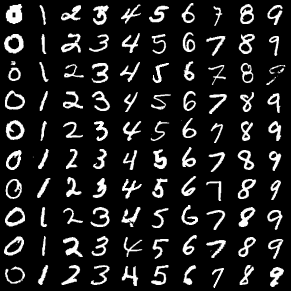
\includegraphics[scale=.9]{transfer/fig/MNIST.png}} \label{fig:single:MNIST}
		 &
		 \subfloat[USPS]{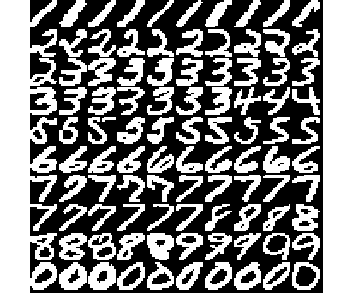
\includegraphics[scale=.9]{transfer/fig/USPS.png}}  \label{fig:single:USPS} 	
	\end{tabular}\caption{Some examples of MNIST \& USPS.}\label{fig:single:dataset}
\end{figure}

% Table generated by Excel2LaTeX from sheet 'Sheet1'
\begin{table}[htbp]\label{tab:single:MNIST}
	\centering
	\caption{Data distribution of MNIST subset}
	\begin{tabular}{|C{2cm}|C{2cm}|C{2cm}|C{2cm}|C{2cm}|C{2cm}|}
		\hline
		digit&\# examples&percentage&digit&\# examples&percentage\\\hline
		1     & 583   & 9.7\% & 6     & 511   & 8.5\% \\
		\hline
		2     & 686   & 11.4\% & 7     & 602   & 10.0\% \\\hline
		3     & 590   & 9.8\% & 8     & 609   & 10.2\% \\\hline
		4     & 652   & 10.9\% & 9     & 607   & 10.1\% \\\hline
		5     & 564   & 9.4\% & 10    & 596   & 9.9\% \\
		\hline
	\end{tabular}%
	\label{tab:addlabel}%
\end{table}%




\subsubsection{USPS}
We also use another handwritten digital dataset USPS \cite{hull1994database}. USPS contains 11,000 images and the data is evenly distributed among 10 classes, i.e. 1,100 examples for each digit. Each digit is represented as a 16x16 greyscale image.

\subsection{Experiment Setup}
In this part, we introduce the experiment set up on the two datasets. We perform experiment on different settings to simulate different scenarios for transfer learning. 

As we discussed in Section \ref{sec:single:comb}, previous work \cite{ben2010theory} show that the more similar of the source model(s) and the target task are, the more improvement the target model can get from the source model(s). When the source model and the target task are unrelated, negative transfer could happen. 
In order to test the robustness of our algorithm, we should assign the source model with different $\mathcal{D}$-relationship to the target task and test how our algorithm performs, especially when negative transfer could happen. To generate the source model(s) with different $\mathcal{D}$-relationship to the target task, we first split the dataset into 3 sub-sets: source training set, target training set and test set. Then we add the noise to the source training set and train the source model(s) from it. Therefore, as we add more noise to the source training set, the source models are more unrelated to the target task.

\begin{figure}\label{fig:single:split}
	\centering
	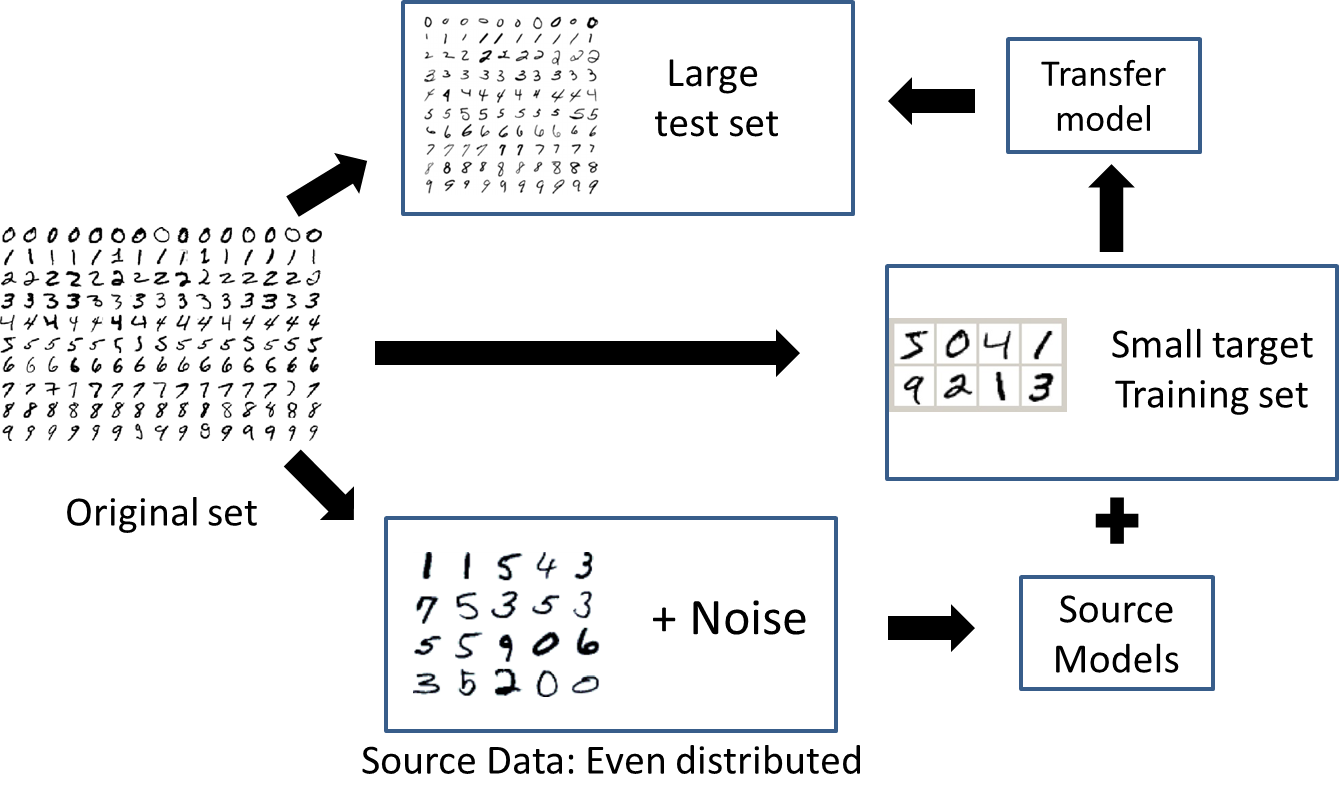
\includegraphics[scale=.7]{transfer/fig/split.png}
	\caption{Illustration of our training procedure. The data is splitted into 3 sets: a source training set, a small target training set and a large test set. Salt \& pepper noise is added into the source training set in order to generate different source models.}
\end{figure}

\begin{figure}\label{fig:single:split}
	\centering
	\subfloat[Noise Rate = 0  ]{
\includegraphics[scale=.7]{transfer/fig/0.png}}\\
	\subfloat[Noise Rate = 0.3]{
\includegraphics[scale=.7]{transfer/fig/1.png}}\\
	\subfloat[Noise Rate = 0.5]{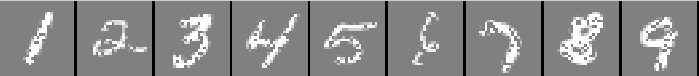
\includegraphics[scale=.7]{transfer/fig/2.png}}\\
	\subfloat[Noise Rate = 0.8]{
\includegraphics[scale=.7]{transfer/fig/3.png}}\\
	\caption{Images with different level of noise rate. By adding more slat\&pepper noise, the images become less clear.}
\end{figure}

% Table generated by Excel2LaTeX from sheet 'Sheet1'
\begin{table}[htbp]
	\centering
	\caption{Setups for our experiment on two datasets}
	\begin{tabular}{|C{5cm}|C{3cm}|C{3cm}|}
		\hline
		& MNIST & USPS \\
		\hline
		noise rate & \multicolumn{2}{c|}{0,0.2,0.3,0.5,0.8,0.9} \\\hline
		source training set size & \multicolumn{2}{c|}{100} \\\hline
		target training set size & \multicolumn{2}{c|}{5,10,15,20,25} \\\hline
		test set size & 4700  & 9700 \\
		\hline
	\end{tabular}%
	\label{tab:addlabel}%
\end{table}%

%\chapter{Learning Food Recognition Model with Deep Representation}

\section{Introduction}
%Deep Learning with Convolutional Neural Networks (CNNs) is the most popular method for image recognition and has been applied to solve many real problems. In this chapter, we investigate problem of using the pre-trained CNNs for transfer learning. In particular, we fine-tune the parameters of the pre-trained CNNs on two food image database and achieve the improved results. We also investigate the changes of parameter after fine-tuning and try to obtain some important experience on fine-tuning the deep CNNs.
 



\section{CNN layers:conv/pool/norm etc}
A CNN consists of some convolutional and subsampling layers optionally followed by fully connected layers. In this part, we introduce the layers used in our work.
\subsection{Convolutional Layer}
Convolutional Layer is the core building block of a Convolutional Network, and its output volume can be interpreted as holding neurons arranged in a 3D volume.
Natural images have the property of being "stationary" meaning that the statistics of one part of the image are the same as any other part. This suggests that the features that we learn at one part of the image can also be applied to other parts of the image, and we can use the same features at all locations.

Formally, given some original $h\times w$ input images $I$, we can train a small autoencoder from $a \times b$ kernel matrix. Also, we have to set other hyperparameters, stride $s$ and padding $p$. Stride defines the number of pixels the kernel should be moved in each step around the image $I$ and padding defines the number of rows/columns padded to the height and width of the original input (see Figure \ref{fig:cnn:conv}). 
Given a $a \times b$ kernel matrix $W^{(1)}$, bias $b^{(1)}$, padding $p$ and stride $s$, we can encode the original image $I$ as $f_{conv}=sigmod(W^{(1)}I_p+b^{(1)})$ for $I_p \in I$, giving us $f_{conv}$ (called feature map of $W^{(1)}$), a  $\left\lceil\frac{(h-a+2p)}{s}+1\right\rceil\times\left\lceil\frac{(w-b+2p)}{s}+1\right\rceil$ array of feature map. In general, for any specific input $I$ ($h \times w \times c$ array matrix) of a convolutional layer $L$, assuming we have $k$ such $a \times b \times c$ kernel matrix, its feature maps $f$ should be a $\left\lceil\frac{(h-a+2p)}{s}+1\right\rceil\times\left\lceil\frac{(w-b+2p)}{s}+1\right\rceil \times k$ array matrix with $f_{conv}^{(i)}=sigmod(W^{(i)}I_p+b^{(i)})$ for $I_p \in I$ and $i \in 1,\dots k$.

In real applications, small kernels ($3\times3$, $5\times5$ and $7\times7$) are preferred by many different CNN architectures \cite{krizhevsky2012imagenet} \cite{lecun1998gradient} \cite{simonyan2014very} \cite{zeiler2014visualizing}. Recent development of tiny $1\times1$ kernel shows an improvement on both accuracy and computational efficiency \cite{szegedy2014going}.
\begin{figure}
	\centering
	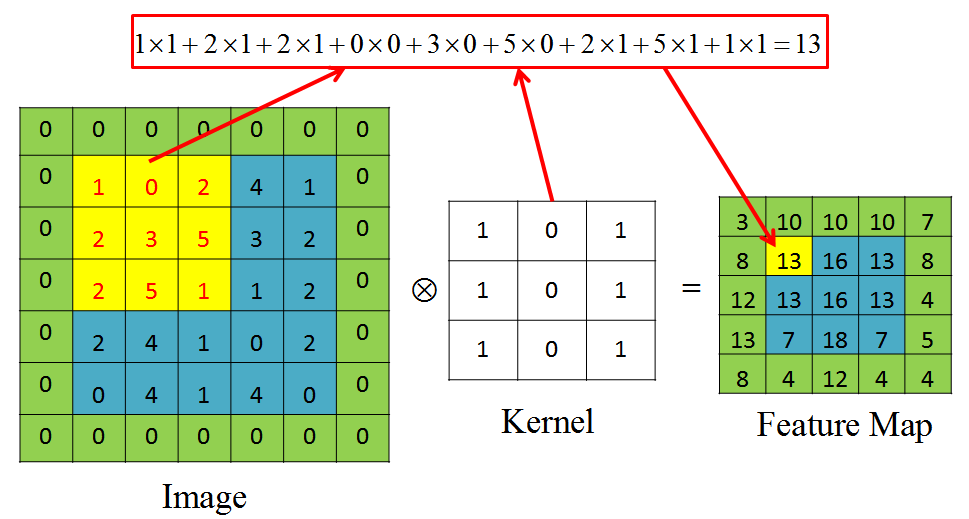
\includegraphics[scale=.6]{cnn/fig/conv.png}
	\caption{Convolution operation with $3\times3$ kernel, stride 1 and padding 1. $\otimes$ denotes the convolutional operator.} \label{fig:cnn:conv}
\end{figure}

\subsection{Pooling Layer}
Pooling layer is widely used in all kinds of CNN architecture for dimensional reduction and computational efficiency. 
After obtaining features maps using convolutional layer, we need to use them for classification. However, applying the feature maps from the convolutional layer for classification would be a computational challenge. Consider for instance images of size $96\times96$ pixels, and suppose we have learned 400 features over $8\times8$ inputs. Each convolution results in an output of size $(96-8+1)\times(96-8+1)=7921$, and since we have 400 features, this results in a vector of $892\times 400=3,168,400$ features per example. Learning a classifier from over 3 million features could lead to severe over-fitting.

Therefore, it is common to periodically insert a (Max) Pooling layer in-between successive convolutional layers in CNN architecture. Its function is to progressively reduce the spatial size of the representation to reduce the amount of parameters and computation in the network, and hence to also control overfitting. The pooling layer works independently on the channel dimension and resizes the feature map spatially. For certain $h \times w \times c$ input array matrix, a $a \times b$ Pooling layer with stride $s$ and $p$ padding would output a $\left\lceil\frac{(h-a+2p)}{s}+1\right\rceil\times\left\lceil\frac{(w-b+2p)}{s}+1\right\rceil \times c$ matrix array.

In general, two kinds of pooling strategy, Max Pooling and Average Pooling, are commonly used in CNN architecture (see Figure \ref{fig:cnn:pool}). Average pooling was often used historically but has recently fallen out of favor compared to the max pooling operation, which has been shown to work better in practice \cite{malmaud2015s} \cite{szegedy2014going}. Max Pooling is been widely used in all kinds CNN architectures \cite{boureau2010theoretical} \cite{yang2009linear}. 
\begin{figure}
	\centering
	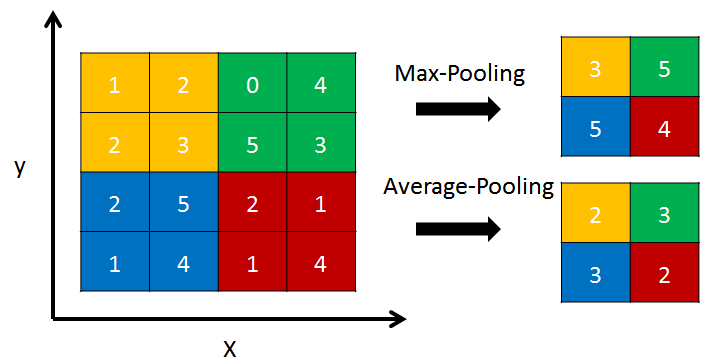
\includegraphics[scale=.8]{cnn/fig/pool.png}
	\caption{$2\times2$ pooling layer with stride 2 and padding 0.}\label{fig:cnn:pool}
\end{figure}

\subsection{Fully Connected Layer}
Fully Connected (FC) Layer have full connections to all activations in the previous layer, as seen in regular Neural Networks. Recent work show that FC layers with Rectified Linear Units and Dropout can greatly improve the learning speed as well as avoid overfitting for deep CNNs \cite{hinton2012improving} \cite{nair2010rectified}.
\subsubsection{Rectified Linear Units (ReLUs) for Activation}
Rectified Linear Units can be considered as replacing each binary unit with sigmoid activation by an infinite number of copies that all have the same weights but have progressively more negative biases. This replacing procedure can be mathematically presented as:
\begin{equation}
\sum\limits_i^N {\sigma (x - i + 0.5)}  \approx \log (1 + {e^x})
\end{equation}
where $\sigma(x)$ is the sigmoid function. In practice, Rectified Linear Units use the function 
\begin{equation}
f(x) = \log (1 + {e^x}) \approx \max(x,0) 
\end{equation}\label{eq:cnn:relu}
as the activation function for approximation \cite{jarrett2009best}. With $max$ function, the derivatives of the active ($x>0$) and inactive neurons are 1 and 0 respectively.  As a result, ReLUs can speed up the learning procedure greatly and improve the performance.
\subsubsection{DropOut}
In FC layer, nodes are connected to each other and this leads to a large number of parameters. Generally, larger number of parameters means more power for Neural Networks and more easily prone to overfitting. Dropout is a technique for addressing this problem.
The key idea is to randomly drop units (along with their connections) from the neural network during training \cite{srivastava2014dropout}. Technically, dropout can be interpreted as adding extra noise into the training procedure. Without actually adding noise, FC layer with dropout is tolerant of higher level of noise (20 \%-50\%). Randomly dropping out the nodes, for any node in FC layer, it can't rely on the other nodes to adjust its result. By eliminating the co-adaptation of hidden units, dropout becomes a technique that can be applied to any general domain and improve the performance of neural nets.   
\begin{figure}
	\centering
	\begin{tabular}{cc}
		\subfloat[ Standard Neural Net ]{    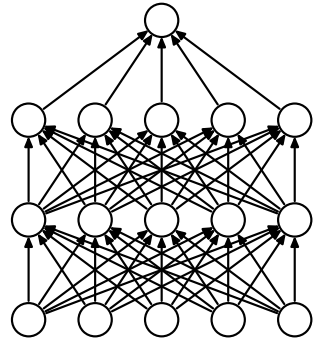
\includegraphics[width=0.3\textwidth]{cnn/fig/net.png}}&
		\subfloat[After Dropout]{    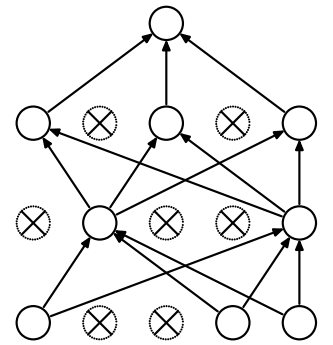
\includegraphics[width=0.3\textwidth]{cnn/fig/dropnet.png}} \\
	\end{tabular}
\end{figure}
\section{Datasets}
In this section, we introduce some details about the two architectures and the food datasets used in our experiments.
\subsection{Models}
In this paper, AlexNet and GoogLeNet are their Caffe \cite{jia2014caffe} implementations and all the results for a specific CNN architecture are obtained from a single model.

\textbf{AlexNet}
contains 5 layers followed by the auxiliary classifier which contains 2 fully connected layers (FC) and 1 softmax layer. Each of the first two layers can be subdivided into 3 components: convolutional layer with rectified linear units (ReLUs), local response normalization layer (LRN) and max pooling layer. Layer 3 and layer 4 contain just convolutional layer with ReLUs while layer 5 is similar to the first two layers except for the LRN. For each of the fully connected layer, 1 ReLUs and 1 dropout \cite{srivastava2014dropout} layer are followed.

\textbf{GoogLeNet}
shows another trend of deep CNN architecture with lots of small receptive fields. There are 9 Inception modules in GoogLeNet and Figure \ref{incept} shows the architecture of a single inception module. Inspired by \cite{linNiN}, lots of $1\times 1$ convolutional layers are used for computational efficiency. Another interesting feature of GoogLeNet is that there are two extra auxiliary classifiers in intermediate layers. During the training procedure, the loss of these two classifiers is counted into the total loss with a discount weight 0.3, in addition to the loss of the classifier on top. More architecture details can be found from \cite{szegedy2014going}.
%\begin{figure}
%\centering
%\includegraphics[scale=.11]{cnn/fig/g_v.pdf}\\
%\end{figure}
\begin{figure}
	\centering
	% Requires \usepackage{graphicx}
	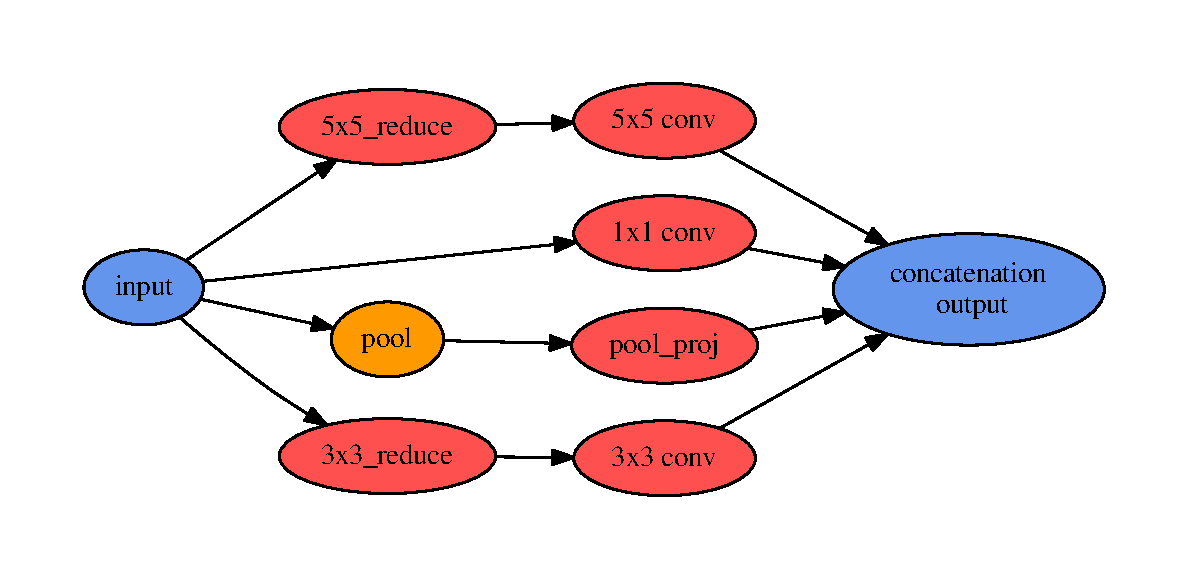
\includegraphics[scale=.7]{cnn/fig/inception.pdf}\\
	\caption{Inception Module. $n\times n$ stands for size $n$ receptive field, $n\times n\_reduce$ stands for the $1\times 1$ convolutional layer before the $n\times n$ convolution layer and $pool\_proj$ is another $1\times 1$ convolutional layer after the MAX pooling layer. The output layer concatenates all its input layers.}\label{incept}
\end{figure}

\subsection{Food Datasets}
Besides ImageNet dataset, there are many popular benchmark datasets for image recognition such as Caltech dataset and CIFAR dataset, both of which contain hundreds of classes. However, in this paper, we try to focus on a more specific area, food classification. Compared to other recognition tasks, there are some properties of the food (dishes) which make the tasks become a real challenge:
\begin{itemize}
	\item Food doesn't have any distinctive spatial layout: for other tasks like scene recognition, we can always find some discriminative features such as buildings or trees, etc;
	\item Food class is a small sub-category among all the categories in daily life, so the inter-class variation is relatively small; on the other hand, the contour of food varies depending on many aspects such as the point of view or even its components.
\end{itemize}
These properties make food recognition catastrophic for some recognition algorithms. Therefore, the training these two architectures on the food recognition task can reveal some important aspects of themselves and help people better understand them. In this paper, we use two image datasets Food-256 \cite{kawano14c}\footnote{Dataset can be found http://foodcam.mobi/dataset.html} and Food-101 \cite{bossard2014food}\footnote{Dataset can be found http://www.vision.ee.ethz.ch/datasets\_extra/food-101}. It is worthy to mention that PFID dataset is also a big public image database for classification, but their images are collected in a laboratory condition which is considerably not applicable for real recognition task.

\textbf{Food-256 Dataset.}
This is a relatively small dataset containing 256 kinds of foods and 31644 images from various countries such as French, Italian, US, Chinese, Thai, Vietnamese, Japanese and Indonesia. The distribution among classes is not even and the biggest class (vegetable tempura) contains 731 images while the smallest one contains just 100 images. For this small dataset, we randomly split the data into training and testing set, using around 80\% (25361 images) and 20\% (6303 images) of the original data respectively and keep the class distribution in these two sets uniform. The collector of this dataset also provides boundary box for each image to separate different foods and our dataset is cropped according to these boundary boxes.

\textbf{Food-101 Dataset.}
This dataset contains 101-class real-world food (dish) images which were taken and labeled manually. The total number of images is 101,000 and there are exactly 1000 images for each class. Also, each class has been divided into training and testing set containing 750 images and 250 images respectively by its collector. The testing set is well cleaned manually while the training set is not well cleaned on purpose. This noisy training set is more similar to our real recognition situation and it is also a good way to see the effect of the noise on these two architectures.

\subsection{Data Augmentation}
In this section, we introduce some data augmentation methods in our work to enrich our training data. Previous work shows that with intensive augmentation for the training data, the performance of CNN model can be improved \cite{wu2015deep}. 
Data Augmentation is an efficient way to enrich the data. There are also some techniques that can apply to enlarge the dataset such as subsampling and mirroring. The original images are firstly resized to $256\times 256$ pixels. We crop the 4 corners and center for each image according to the input size of each model and flap the 5 cropped images to obtain 10 crops. For the testing set, the prediction of an image is the average prediction of the 10 crops (see Figure \ref{fig:cnn:crop}).

\begin{figure}
	\centering
	\begin{tabular}{cccc}
		\multicolumn{2}{c}{\subfloat[Original image]{    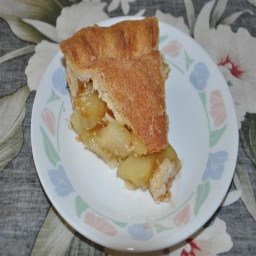
\includegraphics[width=0.15\textheight]{cnn/fig/crop00.png}}}&
		\subfloat[Center]{    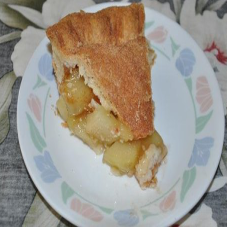
\includegraphics[width=0.15\textheight]{cnn/fig/crop4.png}}&
		\subfloat[Center mirror]{    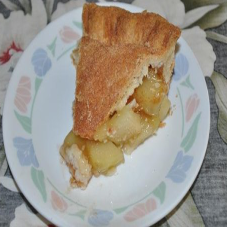
\includegraphics[width=0.15\textheight]{cnn/fig/crop9.png}}  
		\\    
		
		\subfloat[Up-left]{    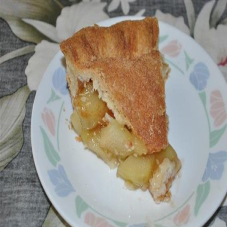
\includegraphics[width=0.15\textheight]{cnn/fig/crop0.png}}&
		\subfloat[Up-left mirror]{    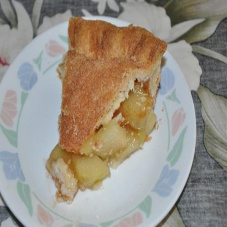
\includegraphics[width=0.15\textheight]{cnn/fig/crop5.png}} & \subfloat[Up-right]{    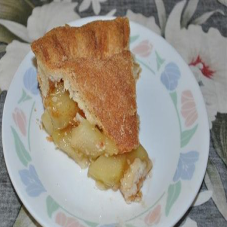
\includegraphics[width=0.15\textheight]{cnn/fig/crop1.png}}&
		\subfloat[Up-right mirror]{    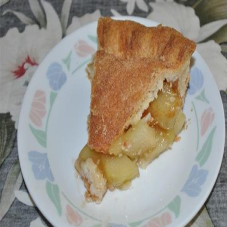
\includegraphics[width=0.15\textheight]{cnn/fig/crop6.png}}\\
		
		\subfloat[Bottom-left]{    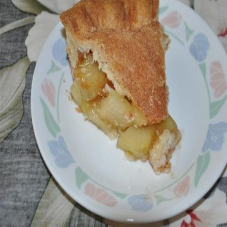
\includegraphics[width=0.15\textheight]{cnn/fig/crop2.png}}&
		\subfloat[Bottom-left mirror]{    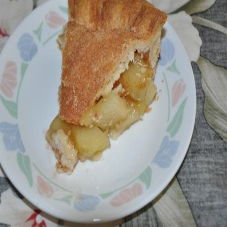
\includegraphics[width=0.15\textheight]{cnn/fig/crop7.png}} & \subfloat[Bottom-right]{    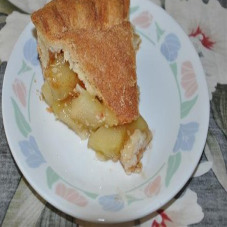
\includegraphics[width=0.15\textheight]{cnn/fig/crop3.png}}&
		\subfloat[Bottom-right mirror]{    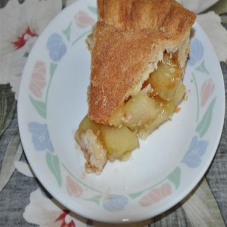
\includegraphics[width=0.15\textheight]{cnn/fig/crop8.png}}\\
		
	\end{tabular}
	\caption{Crop area from original image}\label{fig:cnn:crop}
\end{figure}

Before cropping subsamples from the original image, we also use other augmentation methods such as color casting and vignette etc., to enrich our data and make our model less sensitive to lighting changes and other invariance (see Figure \ref{fig:cnn:argu}). 

Compared to color shifting in \cite{krizhevsky2012imagenet}, we use color casting to alter the intensities of the RGB channels in training images. For each image, we firstly use a random boolean parameter to determine whether its R, G, and B channel should be changed. For any channel that should be changed, we add a random integer ranging from $[-20 , 20]$ to this specific channel. We also apply vignetting effect to the original image. In our implementation, we apply a 2D Gaussian kernel on the original image for vignetting. The two parameter $\sigma_x$ and $\sigma_y$ are randomly chosen from $[160,200)$. We also apply some geometric transformation such as stretching and rotation, on the original image for data augmentation. In summary, we enriched the data by 11 times, 3 times color shifting, 2 times vignetting, 4 times stretching and 1 time rotation and plus the original image.

During the fine-tuning process, we initial the learning rate 0.01 and it decreases 90\% (times 0.1) every 10000 iterations. The detail training configuration is shown in Table \ref{tab:config}.

\begin{figure}
	\centering
	\subfloat[Original image]{    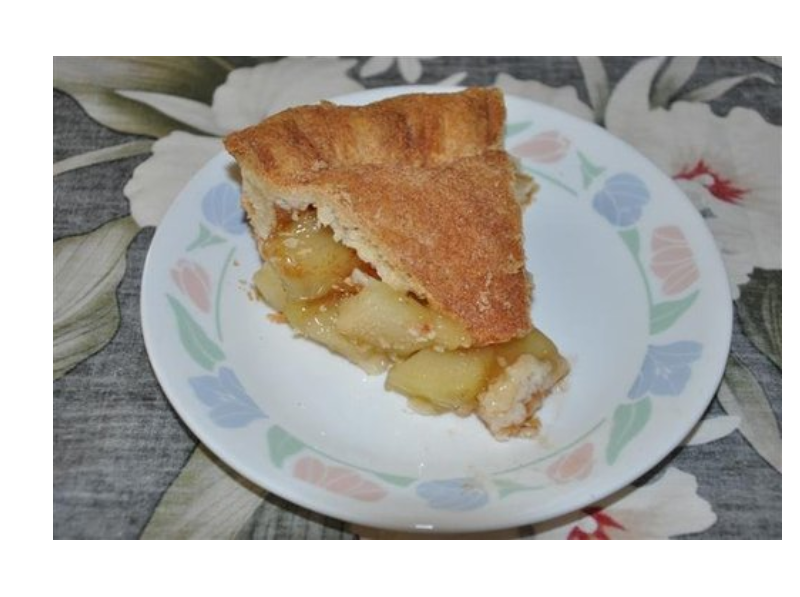
\includegraphics[width=0.3\textwidth]{cnn/fig/org.png}  }
	\subfloat[Red casting]{    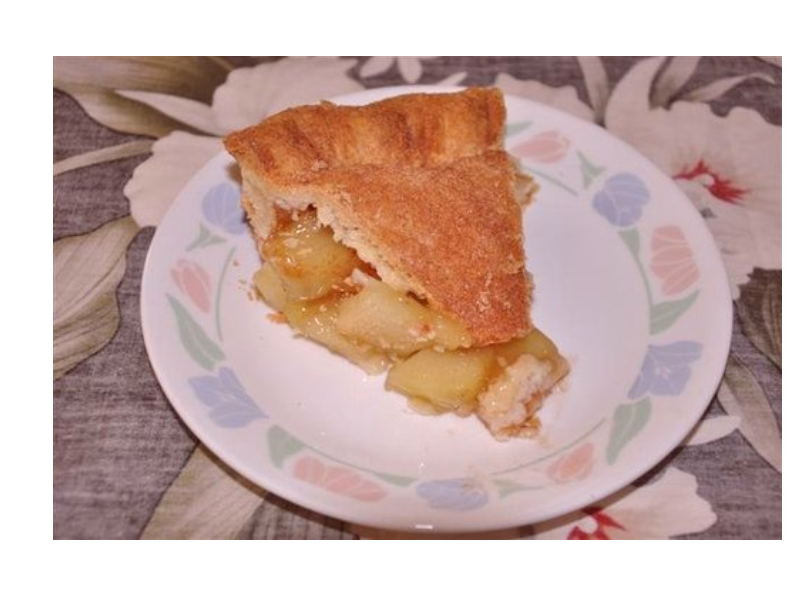
\includegraphics[width=0.3\textwidth]{cnn/fig/red.png}  }
	\subfloat[Green casting]{    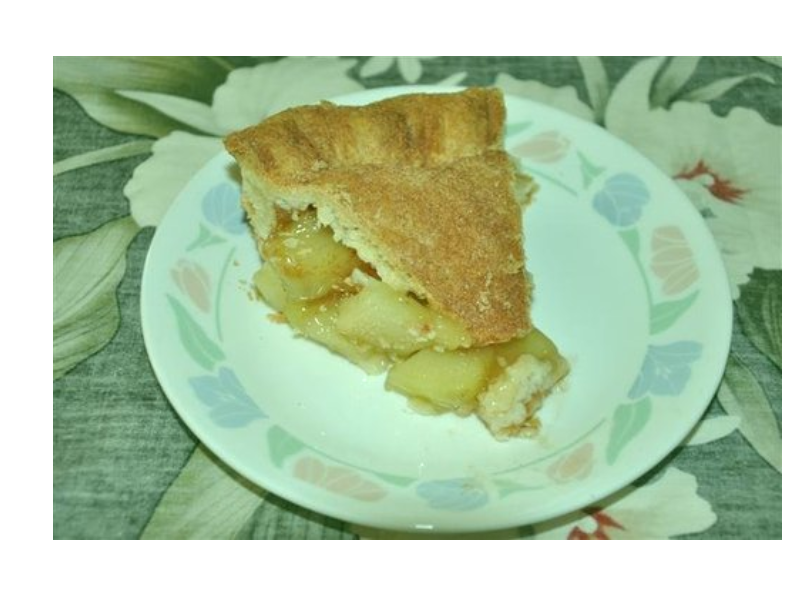
\includegraphics[width=0.3\textwidth]{cnn/fig/green.png}  }\\
	\subfloat[Blue casting]{    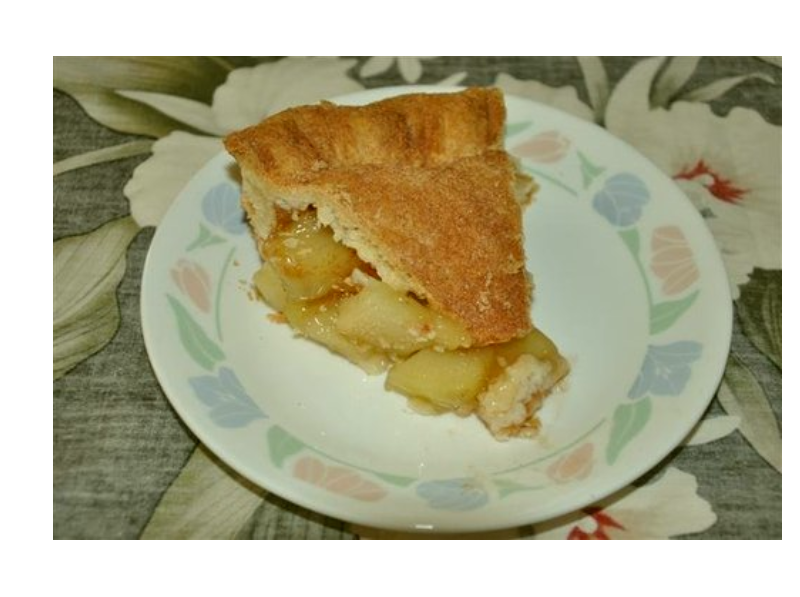
\includegraphics[width=0.3\textwidth]{cnn/fig/blue.png}  }
	\subfloat[RGB casting]{    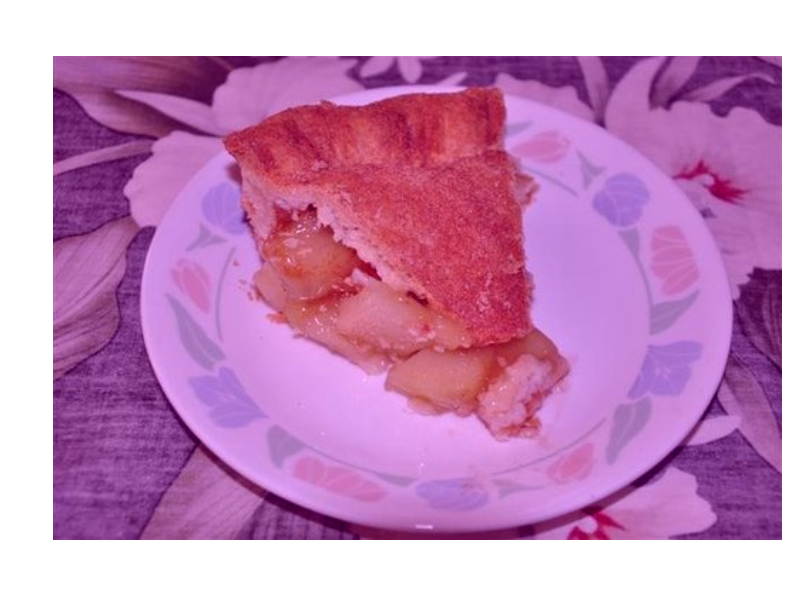
\includegraphics[width=0.3\textwidth]{cnn/fig/rgb.png}  }
	\subfloat[Vignette]{    \includegraphics[width=0.3\textwidth]{cnn/fig/v1.png}  }\\
	\subfloat[More vignette]{    \includegraphics[width=0.3\textwidth]{cnn/fig/v2.png}  }
	\subfloat[Horizontal stretch]{    \includegraphics[width=0.3\textwidth]{cnn/fig/s1.png}  }
	\subfloat[More horizontal stretch]{    \includegraphics[width=0.3\textwidth]{cnn/fig/s2.png}  }\\
	\subfloat[Vertical stretch]{    \includegraphics[width=0.3\textwidth]{cnn/fig/s4.png}  }
	\subfloat[More vertical stretch]{    \includegraphics[width=0.3\textwidth]{cnn/fig/s3.png}  }
	\subfloat[Rotation]{    \includegraphics[width=0.3\textwidth]{cnn/fig/rota.png}  }\\
	
	\caption{Different data augmentation methods}\label{fig:cnn:argu}
\end{figure}


%\subsection{Configuration}
\begin{table}
	\centering
	\begin{tabular}{|c|c|}
		\hline
		Batch Size & 16 \\ \hline
		Learning Rate& 0.01\\ \hline
		Learning Rate Decay Policy& Drop 0.1 every 10000 iterations\\\hline
		Drop Rate & 0.1\\\hline
		Training Iteration& 100000\\\hline
		Momentum & 0.9\\\hline
		Weight Decay Rate& 0.0002\\\hline
		\end{tabular}
		\caption{Experimental configuration for GoogLeNet}\label{tab:config}
	\end{table}

\section{Experimental Discuss}
Training a CNN with millions of parameters on a small dataset could easily lead to horrible overfitting. But the idea of supervised pre-training on some huge image datasets could prevent this problem in a certain degree. Compared to other randomly initialized strategies with a certain distribution, supervised pre-training is to initialize the weights according to the model trained for a specific task. Indeed, initialization using the pre-trained model has certain bias as there is no single dataset including all the invariance for natural images \cite{agrawal2014analyzing}, but this bias can be reduced as the pre-trained image dataset increases and the fine-tuning should benefit from it.
\subsection{Pre-training and Fine-tuning}
We conduct several experiments on both architectures and use different training initialization strategies for both Food-256 and Food-101 datasets. The scratch models are initialized with Gaussian distribution for AlexNet and Xavier algorithm for GoogLeNet%, which automatically determines the scale of initialization based on the number of input and output neurons
\cite{glorot2010understanding}. These two initializations are used for training the original models for the ImageNet task. The ft-last and fine-tuned models are initialized with the weights pre-trained from the ImageNet dataset. For the ft-last model, we just re-train the fully connected layers while the whole network is fine-tuned for the fine-tune model.
\begin{table}[htbp]
	\centering
	\caption{Top-5 Accuracy in percent on fine-tuned, ft-last and scratch model for two architectures}
	\begin{tabular}{|l|cc|cc|}
		\hline
		& \multicolumn{2}{c|}{AlexNet} & \multicolumn{2}{c|}{GoogLeNet} \\  \hline 
		& Food-101   & Food-256   & Food-101   & Food-256 \\\hline
		Fine-tune & \textbf{88.12} & \textbf{85.59} & \textbf{93.51} & \textbf{90.66} \\\hline
		Ft-last &76.49    &79.26&    82.84    &83.77\\\hline
		Scratch & 78.18 & 75.35 & 90.45 & 81.20 \\\hline
	\end{tabular}%
	\label{tab:ft}%
\end{table}%


% Table generated by Excel2LaTeX from sheet 'Sheet1'
\begin{table}[htbp]
	\centering
	\caption{Accuracy compared to other methods on Food-256 dataset in percent}
	\begin{tabular}{|c|C{3cm}|c|c|}
		\hline
		& fv+linear \cite{Kawano:2014} & GoogLeNet & AlexNet \\\hline
		
		Top1  & 50.1& \textbf{70.13} & 63.82 \\\hline
		Top5  & 74.4  & \textbf{90.66} & 85.59\\\hline
	\end{tabular}%
	\label{tab:256}%
\end{table}%

% Table generated by Excel2LaTeX from sheet 'Sheet1'
\begin{table*}[htbp]
	\centering
	\caption{Top-1 accuracy compared to other methods on Food-101 dataset in percent}
	\begin{tabular}{|c|C{3cm}|C{3cm}|c|c|}
		\hline
		& RFDC\cite{bossard2014food} & MLDS($\approx$\cite{singh2012unsupervised}) & GoogLeNet & AlexNet \\\hline
		
		Top1 accuracy & 50.76 & 42.63& \textbf{78.11 }& 66.40 \\\hline
		
	\end{tabular}%
	\label{tab:101}
\end{table*}%
\begin{figure*}[htbp]
	\centering
	% Requires \usepackage{graphicx}
	\includegraphics[scale=0.5]{cnn/fig/sashimi.png}\\
	\caption{Visualization of some feature maps of different GoogLeNet models in different layers for the same input image. 64 feature maps of each layer are shown. Conv1 is the first convolutional layer and Inception\_5b is the last convolutional layer. }
	\label{fig:sashimi}
\end{figure*}
From Table \ref{tab:ft} we can see that fine-tuning the whole network can improve the performance of the CNN for our task. Compared to other traditional computer vision methods (see Table \ref{tab:256} and \ref{tab:101}), GoogLeNet outperforms the other methods with large margins and we provide the state-of-the-art performance of these two food image datasets.

In Figure \ref{fig:sashimi} we visualize the feature maps of the pre-trained GoogLeNet model and fined-tuned GoogLeNet model with the same input image for some layers. We can see that the feature maps of the lower layer are similar as the lower level features are similar for most recognition tasks.
Then we can see that the feature maps in the high-level are different which leads to totally different recognition results.
Since only the last layer (auxiliary classifier) of the ft-last model is optimized, we can infer that the higher level features are more important which is consistent with our intuition. Also from Table \ref{tab:ft}, it is interesting to see that for the Food-101 task, the accuracy of the scratch models outperforms the pre-trained models. Since Food-101 is a relatively large dataset with 750 images per class while Food-256 dataset is an imbalanced small one, this indicates that it is difficult to obtain a good deep CNN model while the data is insufficient.

From Table \ref{tab:ft} we can see that GoogLeNet always performances better than AlexNet on both datasets. This implies that the higher level features of GoogLeNet are more discriminative compared to AlexNet and this is due to the special architecture of its basic unit, Inception module. Table \ref{tab:cosg} and \ref{tab:cosa} show the weights' cosine similarity of each layer between the fine-tuned models and their pre-trained models. From the results we can see that the weights in the low layer are more similar which implies that these two architectures can learn the hierarchical features. As the low-level features are similar for most of the tasks, the difference of the objects is determined by high-level ones which are the combination of these low-level features. Also from Table \ref{tab:cosa}, we can observe that the weights of the pre-trained and fine-tuned models are extremely similar in AlexNet. This can be caused by the size of receptive filed. Since ReLUs are used in both architectures, vanishing gradients do not exist. Rectified activation function is mathematically given by:
\begin{equation}\label{relu}
h = \max ({w^T}x,0) = \left\{ {\begin{array}{*{20}{c}}
	{{w^T}x}&{{w^T}x > 0}\\
	0&{else}
	\end{array}} \right.
\end{equation}

The ReLU is inactivated when its input is below 0 and its partial derivative is 0 as well. Sparsity can improve the performance of the linear classifier on top, but on the other hand, sparse representations make the network more difficult to train as well as fine-tune. The derivative of the filter is $\frac{{\partial J}}{{\partial w}} = \frac{{\partial J}}{{\partial y}}\frac{{\partial y}}{{\partial w}} = \frac{{\partial J}}{{\partial y}}*x$ where $\frac{{\partial J}}{{\partial y}}$ denotes the partial derivative of the activation function, $y=w^Tx$ and $x$ denotes the inputs of the layer. The sparse input could lead to sparse filter derivative for back propagation which would eventually prevent the errors passing down effectively. Therefore, the filters of the fine-tuned AlexNet is extremely similar. Compared to large receptive field used in AlexNet, the inception module in GoogLeNet employs 2 additional $n\times n\_reduced$ convolutional layers before the $3\times 3$ and $5\times 5$ convolutional layers (see Figure \ref{incept}). Even though the original purpose of these two $1\times 1$ convolutional layer is for computational efficiency, these 2 convolutional layers tend to squeeze their sparse inputs and generate the dense outputs for the following layer. We can see from Table \ref{tab:sparse} that the sparsity of the $n\times n\_reduce$ layers are denser than other layers within the inception module. This makes the filters in the following layer more easily to be trained for transfer learning and generate efficient sparse representations.
%\item The pooling strategy. In AlexNet, max pooling is applied to all the pooling layers between several convolution layers. During back propagation, the max pooling layer always passes the error to the place where it came from. Since it only came from one place of the receptive field, the back propagation error is sparse and keeps the most filters unchanged. In GoogLeNet, even though, there is a max pooling layer within every inception module, there are other 3 back-propagation errors, from $5\times 5\_reduce$ and $3\times 3\_reduce$ that can parse dense back-propagation errors to the previous inception module.


\begin{table*}[htbp]
	\centering
	\caption{Cosine similarity of the layers in Inception modules between fine-tuned models and pre-trained model for GoogLeNet}
	\begin{tabular}{|r|cccccc|}
		\hline
		\multicolumn{7}{|c|}{food256} \\\hline
		
		& \multicolumn{1}{l}{1x1} & \multicolumn{1}{l}{3x3\_reduce} & \multicolumn{1}{l}{3x3} & \multicolumn{1}{l}{5x5\_reduce} & \multicolumn{1}{l}{5x5} & \multicolumn{1}{l|}{pool\_proj } \\\hline
		inception\_3a & 0.72  & 0.72  & 0.64  & 0.67  & 0.73  & 0.69 \\
		inception\_3b & 0.59  & 0.64  & 0.53  & 0.70  & 0.60  & 0.56 \\
		inception\_4a & 0.46  & 0.53  & 0.54  & 0.50  & 0.67  & 0.38 \\
		inception\_4b & 0.55  & 0.58  & 0.63  & 0.52  & 0.69  & 0.41 \\
		inception\_4c & 0.63  & 0.64  & 0.63  & 0.57  & 0.68  & 0.52 \\
		inception\_4d & 0.60  & 0.62  & 0.60  & 0.58  & 0.68  & 0.50 \\
		inception\_4e & 0.60  & 0.61  & 0.67  & 0.61  & 0.68  & 0.50 \\
		inception\_5a & 0.51  & 0.53  & 0.58  & 0.48  & 0.60  & 0.39 \\
		inception\_5b & 0.40  & 0.44  & 0.50  & 0.41  & 0.59  & 0.40 \\  \hline
		\multicolumn{7}{|c|}{food101} \\ \hline
		& \multicolumn{1}{l}{1x1 } & \multicolumn{1}{l}{3x3\_reduce} & \multicolumn{1}{l}{3x3} & \multicolumn{1}{l}{5x5\_reduce} & \multicolumn{1}{l}{5x5} & \multicolumn{1}{l|}{pool\_proj } \\\hline
		inception\_3a & 0.71  & 0.72  & 0.63  & 0.67  & 0.73  & 0.68 \\
		inception\_3b & 0.56  & 0.63  & 0.50  & 0.71  & 0.60  & 0.53 \\
		inception\_4a & 0.43  & 0.50  & 0.50  & 0.47  & 0.62  & 0.36 \\
		inception\_4b & 0.48  & 0.52  & 0.57  & 0.50  & 0.67  & 0.35 \\
		inception\_4c & 0.57  & 0.61  & 0.59  & 0.53  & 0.63  & 0.47 \\
		inception\_4d & 0.54  & 0.58  & 0.53  & 0.54  & 0.64  & 0.44 \\
		inception\_4e & 0.53  & 0.54  & 0.61  & 0.55  & 0.62  & 0.42 \\
		inception\_5a & 0.43  & 0.47  & 0.53  & 0.45  & 0.57  & 0.34 \\
		inception\_5b & 0.36  & 0.39  & 0.46  & 0.38  & 0.52  & 0.37 \\
		\hline
	\end{tabular}%
	\label{tab:cosg}%
\end{table*}%


\begin{table*}[htbp]
	\centering
	\caption{Cosine similarity of the layers between fine-tuned models and pre-trained model for AlexNet}
	\begin{tabular}{|r|ccccccc|}
		\hline
		& conv1 & conv2 & conv3 & conv4 & conv5 & fc6   & fc7 \\
		\hline
		food256 & 0.997 & 0.987 & 0.976 & 0.976 & 0.978 & 0.936 & 0.923 \\
		food101 & 0.996 & 0.984 & 0.963 & 0.960 & 0.963 & 0.925 & 0.933 \\
		\hline
	\end{tabular}%
	\label{tab:cosa}%
\end{table*}%

% Table generated by Excel2LaTeX from sheet 'google'
\begin{table*}[htbp]
	\centering
	\caption{Sparsity of the output for each unit in GoogLeNet inception module for training data from Food101 in percent}
	\begin{tabular}{|r|cccccc|}
		\hline
		& 1x1  & 3x3\_reduce & 3x3  & 5x5\_reduce & 5x5  & pool\_proj  \\
		\hline
		inception\_3a & $69.3\pm 1.3$  & $69.6 \pm 1.1$  & $80.0\pm  1.0$& $64.1\pm  2.2$& $75.8\pm  1.6$& $76.2\pm 5.4$\\
		inception\_3b & $92.8 \pm 0.9$&$ 76.5 \pm 0.9$& $94.7\pm 0.9 $&$ 71.6 \pm 2.3 $&$ 94.4\pm 0.5 $&$ 94.7 \pm 1.6$\\
		inception\_4a & $90.9 \pm 0.9$& $70.0\pm 1.2 $& $93.8\pm 1.1 $& $63.3\pm 4.0 $& $91.9\pm 1.8 $& $95.1\pm 2.0$\\
		inception\_4b & $71.9 \pm 1.6$& $67.5\pm 1.2$ & $75.4\pm  1.0$& $58.5 \pm 2.6$& $78.9\pm  1.6$& $85.6\pm 3.6$\\
		inception\_4c & $75.1 \pm 2.4$& $72.6 \pm 1.3$& $81.0\pm 2.0$ & $66.3\pm 6.1 $& $79.7 \pm 3.6$& $88.1\pm 3.3$\\
		inception\_4d & $87.3 \pm 2.7$& $78.0 \pm 2.2$& $88.0\pm 1.6$& $67.9\pm 3.1 $& $88.9\pm 2.8 $& $93.0\pm 2.2$\\
		inception\_4e & $91.8\pm  1.1$& $62.3\pm 2.2 $& $91.0\pm 2.5 $& $49.5 \pm 3.7$& $94.0 \pm 1.0$& $92.3\pm 1.5$\\
		inception\_5a & $78.7 \pm 1.6$& $66.5\pm  1.7$& $82.3\pm 2.6 $& $59.9\pm 3.2 $& $86.4\pm 2.3 $& $87.1\pm 2.6$\\
		inception\_5b & $88.2\pm 2.3 $& $86.8 \pm 1.6$&$ 83.3\pm 4.4$ & $84.0\pm 3.1 $& $81.4\pm 5.3$  & $94.7\pm 1.5$\\
		\hline
	\end{tabular}%
	\label{tab:sparse}%
\end{table*}%

The unique structure of the Inception module guarantees that the sparse outputs from the previous layer can be squeezed with the $1\times 1$ convolutional layers and feed to convolutional layers with a bigger receptive field to generate sparser representation. The squeeze action promises the back propagation error can be transferred more efficiently and makes the whole network more flexible to fit different recognition tasks.

\subsection{Learning across the datasets}
From the previous experiments we can see that pre-training on the ImageNet dataset can improve the performance of the deep convolutional neural network in our specific area. In this part, we will discuss the generalization ability within the food recognition problem.  Zhou et al. trained AlexNet for Scene Recognition across two datasets with identical categories \cite{NIPS2014_Zhou}. But for more complex situation, such as two similar datasets with a little overlapped categories, we are very interested in exploring whether deep CNN can still successfully handle. Therefore, we conduct the following experiment to stimulate a more challenging real world problem: transferring the knowledge from the fine-tuned Food-101 model to a target set, Food-256 dataset. To make the experiment more practical, we limit the number of samples per category from Food-256 for training, because if we want to build our model using deep CNN for a specific task, the resource is always limited and it is exhausted to collect hundreds of labeled images for each category.

\begin{table*}[htbp]
	\centering
	\begin{tabular}{|c|cc|cc|}
		\hline
		& \multicolumn{2}{c|}{AlexNet} & \multicolumn{2}{c|}{GoogLeNet} \\
		\hline
		instances per class & ImageNet  & Food101\_ft    &  ImageNet  & Food101\_ft \\ \hline
		20    & 68.80  & {75.12} & 74.54 & {77.77} \\
		30    & 73.15 & {77.02} & 79.21 & {81.06} \\
		40    & 76.04 & {80.23} & 81.76 & {83.52} \\
		50    & 78.90  & {81.66} & 84.22 & {85.84} \\
		all    & 85.59 &  {87.21} & {90.66 }&   {90.65}     \\
		\hline
	\end{tabular}%
	\caption{Top5 Accuracy for transferring from Food101 to subset of Food256 in percent}
	\label{tab:cross}%
\end{table*}%

The Food-101 and Food-256 datasets share about 46 categories of food even though the images in the same category may vary across these two datasets. The types of food in Food-101 are mainly western style while most types of food in Food-256 are typical Asian foods. We compare the top-5 accuracy trained from different size of the subset for Food-256 on a different pre-trained model and the results are shown in Table \ref{tab:cross}.
%The ImageNet columns denote the pre-trained model trained only on ImageNet images and the Food101\_ft columns denote the pre-trained model trained on ImageNet images and then fine-tuned on Food-101.
The ImageNet columns denote using the model pre-trained from ImageNet dataset as the pre-trained model and Food101\_ft columns denote using the fine-tuned Food-101 model (the same one in Table \ref{tab:ft}) as the pre-trained model.

From the result of Table \ref{tab:cross} we can see that, with this further transfer learning, both CNNs can achieve around 95\% of the accuracy trained on full dataset while just utilizing about half of them (50 per class, 12800 of 25361 images). This indicates that when there is not enough labeled data, with its strong generalization ability, deep CNN trained from a general task can still achieve a satisfying result and perform even better when an additional relevant dataset is involved. This encouraging result may attract more people to use deep CNN for their specific task and continue to explore the potential of the existing architecture as well as designing new ones.



\section{Summary}



%% This adds a line for the Bibliography in the Table of Contents.
\addcontentsline{toc}{chapter}{Bibliography}
%% ***   Set the bibliography style.   ***
\bibliographystyle{plain} % (change according to your preference)
%%% ***   Set the bibliography file.   ***
\bibliography{research}{}
%% ***   NOTE   ***
%% If you don't use bibliography files, comment out the previous line
%% and use \begin{thebibliography}...\end{thebibliography}.  (In that
%% case, you should probably put the bibliography in a separate file
%% and \include or \input it here).

%Appendices.
\begin{appendices}
\chapter{Proofs of Theorems}
%\section{Proof of Theorem1}
%\begin{proof}
For simplification, let $\delta_i=1$ if $i=N+1$ and 0 otherwise, and  ${\theta _{ij}} = {\alpha ''_{ij}}\left( {1 - {\delta _j}} \right)/\psi_{ii}^{ - 1}$. Eq. \eqref{eq:train_loss} can be written as:
\begin{equation}\label{eq:loss_simple}
%\begin{split}
{\xi _i}(\gamma ,\beta )=\mathop {\max }\limits_{n} \bigg \{ {\varepsilon _{n{y_i}}} - 1 + \frac{{\left( {{{\alpha '}_{i{y_i}}} - {{\alpha '}_{in}}} \right)}}{{\psi _{ii}^{ - 1}}} + {\theta _{in}}{\gamma _n} 
- {\theta _{i{y_i}}}{\gamma _{{y_i}}} + \left( {{\delta _n} - {\delta _{{y_i}}}} \right)\sum\limits_k {\frac{{{{\alpha ''}_{ik}}{\beta _k}}}{{\psi_{ii}^{ - 1}}}}  \bigg\}
%\end{split}
\end{equation}
When $\mathbf{\gamma}=\mathbf{\beta} = \mathbf{0}$, from Eq. \eqref{eq:loss_simple} we can get:
\begin{equation*}
{\bar \xi _i} = \mathop {\max }\limits_n \left[ { {\varepsilon _{n{y_i}}}-1 + \frac{{\left( {{{\alpha '}_{i{y_i}}} - {{\alpha '}_{in}}} \right)}}{{\psi _{ii}^{ - 1}}}} \right]
\end{equation*}
To obtain the optimal value of $\gamma$ and $\beta$, we have to seek the saddle point of the Lagrangian problem in \eqref{eq:dual} by finding the minimum for the prime variables $\left\{ \gamma, \beta, \xi \right\}$ and the maximum for the dual variables $\eta $. To find the minimum of the primal problem, we require:
\begin{equation*}
\frac{{\partial L}}{{\partial {\xi _i}}} = 1 - \sum\limits_n {{\eta _{in}}}  = 0 \to \sum\limits_n {{\eta _{in}}}  = 1
\end{equation*}
Similarly, for $\gamma$ and $\beta$, we require:
\begin{eqnarray}\label{eq:opt_gama}
\frac{{\partial L}}{{\partial {\gamma _n}}} &=& {\lambda _1}{\gamma _n} + \sum\limits_i {{\eta _{in}}{\theta _{in}}}  - \sum\limits_{i,n = {y_i}} {\left( {\sum\limits_q {{\eta _{iq}}} } \right){\theta _{in}}{\gamma _n}}  \nonumber\\
&=_1 &{\lambda _1}{\gamma _n} + \sum\limits_i {{\eta _{in}}{\theta _{in}}}  - \sum\limits_i {{\varepsilon _{n{y_i}}}{\theta _{in}}}  = 0  \nonumber\\
&\Rightarrow & \gamma _n^* = \frac{1}{{{\lambda _1}}}\sum\limits_i {\left( {{\varepsilon _{n{y_i}}} - {\eta _{in}}} \right){\theta _{in}}}
\end{eqnarray}
In $=_1$ we use the facts that $\sum_n\eta_{in}=1$ and use $\varepsilon_{ny_i}$ to replace it.
\begin{eqnarray}\label{eq:opt_beta}
\frac{{\partial L}}{{\partial {\beta _n}}} &=& {\lambda _2}{\beta _n} + \left[ {\sum\limits_{i,n} {\frac{{{\eta _{in}}{{\alpha ''}_{in}}}}{{\psi_{ii}^{ - 1}}}\left( {{\delta _n} - {\delta _{{y_i}}}} \right)} } \right] = 0 \nonumber \\
&\Rightarrow &\beta _n^* = \frac{1}{{{\lambda _2}}}\sum\limits_{i,n} {\frac{{{\eta _{in}}{{\alpha ''}_{in}}}}{{\psi _{ii}^{ - 1}}}\left( {{\delta _{{y_i}}} - {\delta _n}} \right)}
\end{eqnarray}
As the strong duality holds,the primal and dual objectives coincide. Plug Eq \eqref{eq:opt_gama} and \eqref{eq:opt_beta} into Eq. \eqref{eq:dual}, we have:
\begin{equation*}
\sum\limits_{i,n} {{\eta _{in}}\left[ {1 - {\varepsilon _{n{y_i}}} + {{\hat Y}_{in}}\left( {\gamma^* ,\beta^* } \right) - {{\hat Y}_{i{y_i}}}\left( {\gamma^* ,\beta^* } \right) - {\xi _i^*}} \right]}=0
\end{equation*}
Expand the equation above, we have:
\begin{eqnarray}\nonumber
\sum\limits_{i,n} {{\eta _{in}}\left[ { {\varepsilon _{n,{y_i}}}-1 + \frac{{\left( {{{\alpha '}_{i{y_i}}} - {{\alpha '}_{in}}} \right)}}{{\psi_{ii}^{ - 1}}} - {\xi _i}} \right]} \nonumber
= {\lambda _1}\sum\limits_r {{{\left\| {\gamma _r^*} \right\|}^2}}  + {\lambda _2}\sum\limits_r {{{\left\| {\beta _r^*} \right\|}^2}}  \ge 0\nonumber
\end{eqnarray}
Rearranging the above, we obtain:
\begin{eqnarray}\label{eq:link1}
\sum\limits_{i,n} {{\eta _{in}}\left[ { {\varepsilon _{n,{y_i}}} -1+ \frac{{\left( {{{\alpha '}_{i{y_i}}} - {{\alpha '}_{in}}} \right)}}{{\psi_{ii}^{ - 1}}}} \right]} 
 \ge \sum\limits_{i,n} {{\eta _{in}}{\xi _i}}  = \sum\limits_i {{\xi _i}}
\end{eqnarray}
The left-hand side of Inequation \eqref{eq:link1} can be bounded by:
\begin{eqnarray}
&&\sum\limits_{i,n} {{\eta _{in}}\left[ { {\varepsilon _{n{y_i}}}-1 + \frac{{\left( {{{\alpha '}_{i{y_i}}} - {{\alpha '}_{in}}} \right)}}{{\psi_{ii}^{ - 1}}}} \right]} \nonumber\\ &&\le \sum\limits_i {\left( {\sum\limits_n {{\eta _{in}}\mathop {\max }\limits_r \left\{ { {\varepsilon _{r{y_i}}} -1 + \frac{{\left( {{{\alpha '}_{i{y_i}}} - {{\alpha '}_{ir}}} \right)}}{{\psi_{ii}^{ - 1}}}} \right\}} } \right)}  \nonumber\\
&&= \sum\limits_i {\left( {\sum\limits_n {{\eta _{in}}{{\bar \xi }_i}} } \right)}  = \sum\limits_i {\bar \xi_i }
\end{eqnarray}
\end{proof} 
\section{Cross Validation Error for LS-SVM}\label{app:cross}
\textbf{Theorem \ref{th:single:cv}}
\textit{	Given a dataset $D=\{(x_i,y_i)|i=1,...,l\}$, the solution of a LS-SVM on $D$ can be written as:}
	
	\begin{equation}\label{eq:app:orgmatrix}
	\left[ {\begin{array}{*{20}{c}}
		{K  + \frac{1}{C}{\rm I}}\\
		1^T
		\end{array}\begin{array}{*{20}{c}}
		1\\
		0
		\end{array}} \right]\left[ {\begin{array}{*{20}{c}}
		\alpha \\
		b
		\end{array}} \right] = \left[ \begin{array}{l}
	y\\
	0
	\end{array} \right]
	\end{equation}
	\textit{Assume that $D^{(n)} = \{(x_i,y_i)|i=1,...,n\}$ is a subset of $D$ and $D\backslash D^{(n)}$ is the complement of $D^{(n)}$ in $D$ , The unbiased leave out error of a LS-SVM trained from $D\backslash D^{(n)}$ on $D^{(n)}$ can be estimated as:}
	
	\begin{equation*}%\label{eq:nout}
	ERR_{leave-out} = \left( {{S_n} - sS_{(l - n + 1)}^{ - 1}{s^T}} \right){\left[ {{\alpha _1},...,{\alpha _n}} \right]^T}
	\end{equation*}
	\textit{Where $\left[\alpha_1,...,\alpha_n\right]$ is the first $n$ rows of $\alpha$ in \eqref{eq:app:orgmatrix}. $S_n$, $s$ and $S_{(l - n + 1)}$ are the square blocks of matrix:}
	
	\begin{equation*}
	\left[ {\begin{array}{c|c}
		{{S_{n }}} &s\\ \hline
		{{s^T}}&{{S_{(l - n + 1)}}}
		\end{array}} \right] =\left[ {\begin{array}{*{20}{c}}
		{K  + \frac{1}{C}{\rm I}}\\
		1^T
		\end{array}\begin{array}{*{20}{c}}
		1\\
		0
		\end{array}} \right]
	\end{equation*}

\begin{proof}
	Following the result of Eq. \eqref{eq:app:orgmatrix} and noticing that the matrix of the left hand in Eq. \eqref{eq:app:orgmatrix} is symmetrical, it can be written as follow:
	
	\begin{equation}\label{eq:app:block}
	\left[ {\begin{array}{*{20}{c}}
		{K  + \frac{1}{C}{\rm I}}\\
		1^T
		\end{array}\begin{array}{*{20}{c}}
		1\\
		0
		\end{array}} \right] = \left[ {\begin{array}{c|c}
		{{S_{n }}} &s\\ \hline
		{{s^T}}&{{S_{(l - n + 1)}}}
		\end{array}} \right] 
	\end{equation}
	Where $S_{n} \in R^{n \times n}$, $s \in R^{n\times (l-n+1)}$ and $S_{(l - n + 1)} \in R^{(l - n + 1) \times (l - n + 1) }$.
	
	For the first round of the cross validation situation, assume the first $n$ examples are used as the validation set. In this case, let $\left[ {{\alpha ^{ - 1}},{b^{ - 1}}} \right] \in R^{l-n+1}$ denote the optimal parameters for a LS-SVM $f^{-1}$ trained on the rest of the samples and they can be found by:
	
	\begin{equation}\label{eq:app:ab,l-n+1}
	\left[ \begin{array}{l}
	{\alpha ^{ - 1}}\\
	{b^{ - 1}}
	\end{array} \right]{\rm{ = S}}_{(l - n + 1)}^{ - 1}{\left[ {{y_{n + 1}},...,{y_l},0} \right]^T}
	\end{equation}
	The prediction of $f^{-1}$ on the validation set $\hat{Y} = \left[\hat{y}_1,...,\hat{y}_n\right]$ is given by:
	
	\begin{equation}\label{eq:app:predict}
	\left[ {\hat {{y}}_1,...,\hat {{y}}}_n \right]^T = s\left[ {\begin{array}{*{20}{c}}
		\alpha^{-1} \\
		b^{-1}
		\end{array}} \right] = sS_{(l - n + 1)}^{ - 1}{\left[ {{y_{n + 1}},...,{y_l},0} \right]^T}
	\end{equation}
	Moreover, the last $l-n+1$ rows in Eq. \eqref{eq:app:orgmatrix} can be represented as $\left[ {\begin{array}{*{20}{c}}{{s^T}}&{{S_{l - n + 1}}}\end{array}} \right] \left[ {\alpha ,b}\right] ^T= \left[ {{y_{n + 1}},...,{y_l},0} \right]^T$. So
	
	\begin{equation}\label{eq:app:yestimate}
	\begin{array}{l}
	\hat{Y}={\left[ {\hat {{y}}_1,...,\hat {{y}}}_n \right]^T} = sS_{(l - n + 1)}^{ - 1}\left[ {\begin{array}{*{20}{c}}
		{{s^T}}&{{S_{l - n + 1}}}
		\end{array}} \right]\left[ {\begin{array}{*{20}{c}}
		\alpha \\
		b
		\end{array}} \right]\\
	= sS_{(l - n + 1)}^{ - 1}{s^T}{\left[ {{\alpha _1},...,{\alpha _n}} \right]^T} + s{\left[ {{\alpha _{n + 1}},...,{\alpha _l},b} \right]^T}
	\end{array}
	\end{equation}
	Then first $n$ rows in Eq. \eqref{eq:app:orgmatrix} can be represented as:
	
	\begin{equation}\label{eq:app:ytrue}
	Y={\left[ {{y_1},...{y_n}} \right]^T} = \left[ {\begin{array}{*{20}{c}}
		{{S_n}}&s
		\end{array}} \right]\left[ {\begin{array}{*{20}{c}}
		\alpha \\
		b
		\end{array}} \right] = {S_n}{\left[ {{\alpha _1},...,{\alpha _n}} \right]^T} + s{\left[ {{\alpha _{n + 1}},...,{\alpha _l},b} \right]^T}
	\end{equation}
	Thus, combining \eqref{eq:app:yestimate} and \eqref{eq:app:ytrue}, we have the following equation:
	
	\begin{equation}
	\begin{array}{l}
	\hat Y = Y - {S_n}{\left[ {{\alpha _1},...,{\alpha _n}} \right]^T} + sS_{(l - n + 1)}^{ - 1}{s^T}{\left[ {{\alpha _1},...,{\alpha _n}} \right]^T}\\
	= Y - \left( {{S_n} - sS_{(l - n + 1)}^{ - 1}{s^T}} \right){\left[ {{\alpha _1},...,{\alpha _n}} \right]^T}
	\end{array}
	\end{equation}
	According to block matrix inversion lemma
	
	\begin{equation}%\label{}
	{\left[ {\begin{array}{*{20}{c}}
			{{S_n}}\\
			{{s^T}}
			\end{array}\begin{array}{*{20}{c}}
			s\\
			{{S_{(l - n + 1)}}}
			\end{array}} \right]^{ - 1}} = \left[ {\begin{array}{*{20}{c}}
		{{\kappa ^{ - 1}}}&{ - {\kappa ^{ - 1}}sS_{(l - n + 1)}^{ - 1}}\\
		{ - {S_{(l - n + 1)}}{s^T}{\kappa ^{ - 1}}}&{S_{(l - n + 1)}^{ - 1} + S_{(l - n + 1)}^{ - 1}{s^T}{\kappa ^{ - 1}}sS_{(l - n + 1)}^{ - 1}}
		\end{array}} \right]
	\end{equation}
	Where $\kappa  = \left( {{S_n} - sS_{(l - n + 1)}^{ - 1}{s^T}} \right)$. We have:
	
	\begin{equation}%\label{eq:nout}
	Y - \hat Y = {\kappa}{\left[ {{\alpha _1},...,{\alpha _n}} \right]^T}
	\end{equation}
\end{proof}
\section{Converage of EMTLe}\label{app:converg}
\begin{theorem}\label{th:1}
Let $L(\beta)$ be a $\lambda$-strongly convex function and $\beta^*$ be its optimal solution.Let $\beta_1,...,\beta_{T+1}$ be a sequence such that $\beta_1 \in B$ and for $t>1$, we have $\beta_{t+1} = \beta_t - \eta_t \Delta_t$ , where $\Delta_t$ is the sub-gradient of $L(\beta_t)$ and $\eta_t = 1/(\lambda t)$. Assume we have $||\Delta_t|| \leq G$ for all $t$. Then we have:	
	\begin{equation}
	L(\beta_{T+1}) \leq L(\beta^*)+\frac{G^2(1+\ln (T))}{2\lambda T}
	\end{equation}
\end{theorem}
\textbf{Proof:}
	As $L(\beta)$ is strongly convex and $\Delta_t$ is in its sub-gradient set at $\beta_t$, according to the definition of $\lambda$-strong convexity \cite{rockafellar2015convex}, the following inequality holds:	
	\begin{equation}\label{eq:app:strong}
		\left\langle {\beta_t - \beta^*,\Delta_t} \right\rangle \geq L(\beta_t)-L(\beta^*)+\frac{\lambda}{2}||\beta_t - \beta^*||^2
	\end{equation} 
	For the term $\left\langle {\beta_t - \beta^*,\Delta_y} \right\rangle$, it can be written as:	
	\begin{equation} \label{eq:app:inner}
	\begin{aligned}
	\left\langle {\beta_t - \beta^*,\Delta_t} \right\rangle &= \left\langle {\beta_t - \frac{1}{2}\eta_t\Delta_t + \frac{1}{2}\eta_t\Delta_t- \beta^*,\Delta_t} \right\rangle\\
	&=\frac{1}{2}\left\langle {\left[ {\left( {{\beta _t} - {\eta _t}{\Delta _t}} \right) - {\beta ^*}} \right] + \left( {{\beta _t} - {\beta ^*}} \right) + {\eta _t}{\Delta _t},{\Delta _t}} \right\rangle \\
	&= \frac{1}{2}\left\langle {\left( {{\beta _{t + 1}} - {\beta ^*}} \right) + \left( {{\beta _t} - {\beta ^*}} \right),{\Delta _t}} \right\rangle  + \frac{1}{2}{\eta _t}\Delta _t^2\\
	&=\frac{1}{2}\left\langle {{\beta _{t + 1}} + {\beta _t} - 2{\beta ^*},{\Delta _t}} \right\rangle  + \frac{1}{2}{\eta _t}\Delta _t^2
	\end{aligned}
	\end{equation}	
	Then we have:
	\begin{equation}\label{eq:app:squrediff}
	\begin{aligned}
	||\beta_t-\beta^*||^2-||\beta_{t+1}-\beta^*||^2 
	%&= ( {{\beta _t} - {\beta _{t + 1}}})  ({{\beta _t} + {\beta _{t + 1}} - 2{\beta ^*}}) 
	=\left\langle {{\beta _{t + 1}} + {\beta _t} - 2{\beta ^*},{\eta_t\Delta _t}} \right\rangle
	\end{aligned}
	\end{equation}
	Using the assumption $||\Delta_t|| \leq G$, we can rearrange \eqref{eq:app:strong} and plug \eqref{eq:app:inner} and \eqref{eq:app:squrediff} into it, we have:	
	\begin{equation}\label{eq:app:it_diff}
	\begin{aligned}
	{Diff}_t &= L(\beta_t)-L(\beta^*)\\\
	 &\leq \frac{{||{\beta _t} - {\beta ^*}|{|^2} - ||{\beta _{t + 1}} - {\beta ^*}|{|^2}}}{{2{\eta _t}}} - \frac{\lambda }{2}||{\beta _t} - {\beta ^*}|{|^2} + \frac{1}{2}{\eta _t}\Delta _t^2 \\
	&\leq \frac{{||{\beta _t} - {\beta ^*}|{|^2} - ||{\beta _{t + 1}} - {\beta ^*}|{|^2}}}{{2{\eta _t}}} - \frac{\lambda }{2}||{\beta _t} - {\beta ^*}|{|^2} + \frac{1}{2}{\eta _t} G^2\\
	&\le\frac{\lambda (t-1)}{2}{||{\beta _t} - {\beta ^*}||^2}- \frac{\lambda t}{2}{||{\beta _{t+1}} - {\beta ^*}||^2}+\frac{1}{2}{\eta _t} G^2
	\end{aligned}
	\end{equation}	
	Due to the convexity, for each pair of $L(\beta_t)$ and $L(\beta_{t+1})$ for $t=1,...,T$, 
	we have the following sequence $L(\beta^*) \leq L(\beta_T) \leq L(\beta_{T-1}) \leq...\leq L(\beta_1)$. 
	For the sequence $Diff_t$ for $t=1,...,T$, we have:
	
	\begin{equation} \label{eq:app:difsum}
	\sum_{t=1}^{T} Diff_t =  \sum_{t=1}^{T}L(\beta_t)-TL(\beta^*) \geq T\left[L(\beta_T)-L(\beta^*)\right]
	\end{equation}	
	Next, we show that 	
	\begin{equation}
	\begin{aligned}
	\sum_{t=1}^{T} Diff_t =&
	\sum_{t=1}^{T}\left\{\frac{\lambda (t-1)}{2}{||{\beta _t} - {\beta ^*}||^2}- \frac{\lambda t}{2}{||{\beta _{t+1}} - {\beta ^*}||^2}+\frac{1}{2}{\eta _t} G^2\right\} \\
	=&-\frac{\lambda T}{2}{||{\beta _{T+1}-\beta^*}||^2} + \frac{G^2}{2 \lambda}\sum_{t=1}^{T} \frac{1}{t}\leq \frac{G^2}{2 \lambda}\sum_{t=1}^{T} \frac{1}{t} \leq \frac{G^2}{2 \lambda}(1+\ln(T))
	\end{aligned}
	\end{equation}	
	Combining \eqref{eq:app:difsum} and rearranging the result, we have:
	\begin{equation*}
	L(\beta_{T+1}) \leq L(\beta^*)+\frac{G^2(1+\ln (T))}{2\lambda T}
	\end{equation*}

%%\chapter{Tables}
%%\section{Configuration of GoogLeNet}
%%\begin{landscape}
%%% Table generated by Excel2LaTeX from sheet 'new  2'
\begin{table}[h]
  \centering
  \caption{Configuration of GoogLeNet}
  \footnotesize
    \begin{tabular}{|c|c|c|c|c|c|c|c|c|c|}
    \hline
    type  & patch size / stride & output size & depth & \#1x1 & \#3x3 reduce & \#3x3 & \#5x5 reduce & \#5x5 pool & proj \\\hline
    convolution & 7x7/2 & 112x112x64 & 1     &       &       &       &       &       &  \\\hline
    max pool & 3x3/2 & 56x56x64 & 0     &       &       &       &       &       &  \\\hline
    convolution & 3x3/1 & 56x56x192 & 2     &       & 64    & 192   &       &       &  \\\hline
    max pool & 3x3/2 & 28x28x192 & 0     &       &       &       &       &       &  \\\hline
    inception(3a) &       & 28x28x256 & 2     & 64    & 96    & 128   & 16    & 32    & 32 \\\hline
    inception(3b) &       & 28x28x480 & 2     & 128   & 128   & 192   & 32    & 96    & 64 \\\hline
    maxpool & 3x3/2 & 14x14x480 & 0     &       &       &       &       &       &  \\\hline
    inception(4a) &       & 14x14x512 & 2     & 192   & 96    & 208   & 16    & 48    & 64 \\\hline
    inception(4b) &       & 14x14x512 & 2     & 160   & 112   & 224   & 24    & 64    & 64 \\\hline
    inception(4c) &       & 14x14x512 & 2     & 128   & 128   & 256   & 24    & 64    & 64 \\\hline
    inception(4d) &       & 14x14x528 & 2     & 112   & 144   & 288   & 32    & 64    & 64 \\\hline
    inception(4e) &       & 14x14x832 & 2     & 256   & 160   & 320   & 32    & 128   & 128 \\\hline
    maxpool & 3x3/2 & 7x7x832 & 0     &       &       &       &       &       &  \\\hline
    inception(5a) &       & 7x7x832 & 2     & 256   & 160   & 320   & 32    & 128   & 128 \\\hline
    inception(5b) &       & 7x7x1024 & 2     & 384   & 192   & 384   & 48    & 128   & 128 \\\hline
    avg pool & 7x7/1 & 1x1x1024 & 0     &       &       &       &       &       &  \\\hline
    dropout (40\%) &       & 1x1x1024 & 0     &       &       &       &       &       &  \\\hline
    linear &       & 1x1x1000 & 1     &       &       &       &       &       &  \\\hline
    softmax &       & 1x1x1000 & 0     &       &       &       &       &       &  \\\hline
    \end{tabular}%
  \label{tab:cnn:googlenet}%
\end{table}%

%%\end{landscape}
%%
%\chapter{Detailed Experiment Results}
%\section{Detailed result on MNIST}
%%\section{Detailed result on MNIST}
\subsection{No Noise}
\begin{figure}[h]
	\centering
	\begin{tabular}{cc}
		\includegraphics[width=0.45\textwidth]{appendix/tables/MNIST_Rate_0_class_1.jpg} & 
		\includegraphics[width=0.45\textwidth]{appendix/tables/MNIST_Rate_0_class_2.jpg} \\
		class 1 & class 2\\
		\includegraphics[width=0.45\textwidth]{appendix/tables/MNIST_Rate_0_class_3.jpg} & 
		\includegraphics[width=0.45\textwidth]{appendix/tables/MNIST_Rate_0_class_4.jpg} \\
		class 3 & class 4\\
	\end{tabular}
\end{figure}
\begin{figure}[h]
	\centering
	\begin{tabular}{cc}
		\includegraphics[width=0.45\textwidth]{appendix/tables/MNIST_Rate_0_class_5.jpg} & 
		\includegraphics[width=0.45\textwidth]{appendix/tables/MNIST_Rate_0_class_6.jpg} \\
		class 5 & class 6\\
		\includegraphics[width=0.45\textwidth]{appendix/tables/MNIST_Rate_0_class_7.jpg} & 
		\includegraphics[width=0.45\textwidth]{appendix/tables/MNIST_Rate_0_class_8.jpg} \\
		class 7 & class 8\\
		\includegraphics[width=0.45\textwidth]{appendix/tables/MNIST_Rate_0_class_9.jpg} & 
		\includegraphics[width=0.45\textwidth]{appendix/tables/MNIST_Rate_0_class_10.jpg} \\
		class 9 & class 10\\
	\end{tabular}
\end{figure}
\clearpage



\subsection{0.3 Noise}
\begin{figure}[h]
	\centering
	\begin{tabular}{cc}
		\includegraphics[width=0.45\textwidth]{appendix/tables/MNIST_Rate_3_class_1.jpg} & 
		\includegraphics[width=0.45\textwidth]{appendix/tables/MNIST_Rate_3_class_2.jpg} \\
		class 1 & class 2\\
		\includegraphics[width=0.45\textwidth]{appendix/tables/MNIST_Rate_3_class_3.jpg} & 
		\includegraphics[width=0.45\textwidth]{appendix/tables/MNIST_Rate_3_class_4.jpg} \\
		class 3 & class 4\\
	\end{tabular}
\end{figure}
\begin{figure}[h]
	\centering
	\begin{tabular}{cc}
		\includegraphics[width=0.45\textwidth]{appendix/tables/MNIST_Rate_3_class_5.jpg} & 
		\includegraphics[width=0.45\textwidth]{appendix/tables/MNIST_Rate_3_class_6.jpg} \\
		class 5 & class 6\\
		\includegraphics[width=0.45\textwidth]{appendix/tables/MNIST_Rate_3_class_7.jpg} & 
		\includegraphics[width=0.45\textwidth]{appendix/tables/MNIST_Rate_3_class_8.jpg} \\
		class 7 & class 8\\
		\includegraphics[width=0.45\textwidth]{appendix/tables/MNIST_Rate_3_class_9.jpg} & 
		\includegraphics[width=0.45\textwidth]{appendix/tables/MNIST_Rate_3_class_10.jpg} \\
		class 9 & class 10\\
	\end{tabular}
\end{figure}
\clearpage



\subsection{0.5 Noise}
\begin{figure}[h]
	\centering
	\begin{tabular}{cc}
		\includegraphics[width=0.45\textwidth]{appendix/tables/MNIST_Rate_5_class_1.jpg} & 
		\includegraphics[width=0.45\textwidth]{appendix/tables/MNIST_Rate_5_class_2.jpg} \\
		class 1 & class 2\\
		\includegraphics[width=0.45\textwidth]{appendix/tables/MNIST_Rate_5_class_3.jpg} & 
		\includegraphics[width=0.45\textwidth]{appendix/tables/MNIST_Rate_5_class_4.jpg} \\
		class 3 & class 4\\
	\end{tabular}
\end{figure}
\begin{figure}[h]
	\centering
	\begin{tabular}{cc}
		\includegraphics[width=0.45\textwidth]{appendix/tables/MNIST_Rate_5_class_5.jpg} & 
		\includegraphics[width=0.45\textwidth]{appendix/tables/MNIST_Rate_5_class_6.jpg} \\
		class 5 & class 6\\
		\includegraphics[width=0.45\textwidth]{appendix/tables/MNIST_Rate_5_class_7.jpg} & 
		\includegraphics[width=0.45\textwidth]{appendix/tables/MNIST_Rate_5_class_8.jpg} \\
		class 7 & class 8\\
		\includegraphics[width=0.45\textwidth]{appendix/tables/MNIST_Rate_5_class_9.jpg} & 
		\includegraphics[width=0.45\textwidth]{appendix/tables/MNIST_Rate_5_class_10.jpg} \\
		class 9 & class 10\\
	\end{tabular}
\end{figure}
\end{appendices}

%CV only relevant stuff... not full CV.
\addcontentsline{toc}{chapter}{Curriculum Vitae}
\chapter*{Curriculum Vitae}
\begin{table}[ht]
\begin{tabular}{ll}
\textbf{Name:} & \firstname{} \lastname\\\\
\textbf{Post-Secondary} & La La School\\
\textbf{Education and}& La La Land\\
\textbf{Degrees:}& 1996 - 2000 M.A.\\\\
& University of Western Ontario\\
& London, ON\\
& 2008 - 2012 Ph.D.\\\\
\textbf{Honours and}& NSERC PGS M\\
\textbf{Awards:}& 2006-2007\\\\
\textbf{Related Work}& Teaching Assistant\\
\textbf{Experience:}& The University of Western Ontario\\
& 2008 - 2012\\
\end{tabular}
\end{table}
\subsubsection*{Publications:}
La La
\end{document}

